\documentclass{article}
\usepackage[utf8]{inputenc}
\usepackage[T1]{fontenc}
\usepackage{graphicx} % Required for inserting images
\usepackage{amsmath}  % Required for advanced math symbols and alignment
\usepackage{amssymb}  % Required for mathbb and mathcal symbols
\usepackage{tcolorbox} % Required for the styled warning boxes
\usepackage{tikz}     % Required for drawing graphical models
\usepackage{pgfplots}
\usepackage{bm}
\usepackage{float}
\pgfplotsset{compat=1.18}

\title{Univariate Models}
\author{crazymakibe}
\date{June 2026}

\begin{document}

\maketitle

\section*{Independence and Conditional Independence}

\subsubsection*{1. Marginal (Unconditional) Independence}
Two random variables $X$ and $Y$ are \textbf{unconditionally independent} (or \textbf{marginally independent}), denoted as $X \perp Y$, if and only if their joint distribution can be factored completely into the product of their marginal distributions:
\begin{equation}
    X \perp Y \iff p(X, Y) = p(X)p(Y)
\end{equation}

\noindent For a collection of random variables $\{X_1, \dots, X_n\}$ to be \textbf{mutually independent}, the joint distribution of any subset of size $m \le n$ must factorize as:
\begin{equation}
    p(X_1, \dots, X_m) = \prod_{i=1}^{m} p(X_i)
\end{equation}

\begin{tcolorbox}[colback=yellow!5!white, colframe=yellow!60!black, title=Important Distinction]
For mutual independence among a set of variables, pairwise independence is a necessary but not sufficient condition. Every sub-combination must satisfy the product rule.
\end{tcolorbox}

\subsubsection*{2. Conditional Independence (CI)}
In real-world systems, unconditional independence is rare because variables usually share underlying background influences. We say $X$ and $Y$ are \textbf{conditionally independent} given a third variable $Z$, denoted as $X \perp Y \mid Z$, if and only if:
\begin{equation}
    X \perp Y \mid Z \iff p(X, Y \mid Z) = p(X \mid Z)p(Y \mid Z)
\end{equation}

An equivalent and highly intuitive definition can be derived using the definition of conditional probability:
\begin{equation}
    p(X \mid Y, Z) = \frac{p(X, Y \mid Z)}{p(Y \mid Z)} = \frac{p(X \mid Z)p(Y \mid Z)}{p(Y \mid Z)} = p(X \mid Z)
\end{equation}
This demonstrates that once $Z$ is known, observing $Y$ provides no additional information regarding the state of $X$.

\subsubsection*{3. Graphical Model Intuition}
This directional relationship can be represented by a simple Markov chain graph:
\begin{center}
    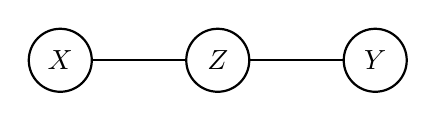
\begin{tikzpicture}[node distance=2cm, auto, >=latex, thick, main node/.style={circle,draw,minimum size=0.8cm}]
        \node[main node] (1) {$X$};
        \node[main node] (2) [right of=1] {$Z$};
        \node[main node] (3) [right of=2] {$Y$};
        \path[-]
        (1) edge node {} (2)
        (2) edge node {} (3);
    \end{tikzpicture}
\end{center}
The path $X - Z - Y$ structurally portrays that all dependency between $X$ and $Y$ is completely mediated via $Z$. These structural dependencies form the mathematical bedrock of \textbf{graphical models}.

\section*{Summary Statistics of a Distribution}

\subsubsection*{1. Mean (Expected Value)}
The mean or expected value, denoted by $\mu$, represents the center of mass of a probability distribution.
For a continuous random variable $X$:
\begin{equation}
    \mathbb{E}[X] \triangleq \int_{-\infty}^{\infty} x p(x) dx
\end{equation}
For a discrete random variable $X$ taking values in a countable set $\mathcal{X}$:
\begin{equation}
    \mathbb{E}[X] \triangleq \sum_{x \in \mathcal{X}} x p(x)
\end{equation}

\noindent \textbf{Properties of Expectation:}
\begin{itemize}
    \item \textbf{Linearity of Expectation:} For constants $a, b$, and any random variables $X_i$ (regardless of mutual independence):
    \begin{equation}
        \mathbb{E}[aX + b] = a\mathbb{E}[X] + b
    \end{equation}
    \begin{equation}
        \mathbb{E}\left[\sum_{i=1}^{n} X_i\right] = \sum_{i=1}^{n} \mathbb{E}[X_i]
    \end{equation}
    \item \textbf{Product of Independent Variables:} If $X_1, \dots, X_n$ are mutually independent:
    \begin{equation}
        \mathbb{E}\left[\prod_{i=1}^{n} X_i\right] = \prod_{i=1}^{n} \mathbb{E}[X_i]
    \end{equation}
\end{itemize}

\subsubsection*{2. Variance and Standard Deviation}
The variance $\sigma^2$ or $\mathbb{V}[X]$ measures the expected squared deviation or "spread" around the mean $\mu$:
\begin{align}
    \mathbb{V}[X] &\triangleq \mathbb{E}\left[(X - \mu)^2\right] = \int_{-\infty}^{\infty} (x - \mu)^2 p(x) dx \\
    &= \int_{-\infty}^{\infty} x^2 p(x)dx - 2\mu\int_{-\infty}^{\infty} xp(x)dx + \mu^2\int_{-\infty}^{\infty} p(x)dx \\
    &= \mathbb{E}[X^2] - \mu^2 \label{eq:var_shortcut}
\end{align}
Rearranging Equation \ref{eq:var_shortcut} yields a highly crucial identity for moment calculations:
\begin{equation}
    \mathbb{E}[X^2] = \sigma^2 + \mu^2
\end{equation}
The standard deviation reverts back to the original units of $X$:
\begin{equation}
    \text{std}[X] \triangleq \sqrt{\mathbb{V}[X]} = \sigma
\end{equation}

\noindent \textbf{Properties of Variance:}
\begin{itemize}
    \item \textbf{Shifting and Scaling:} Shifting a distribution does not alter its spread, while scaling amplifies variance quadratically:
    \begin{equation}
        \mathbb{V}[aX + b] = a^2\mathbb{V}[X]
    \end{equation}
    \item \textbf{Sum of Independent Variables:} If the $n$ variables are mutually independent:
    \begin{equation}
        \mathbb{V}\left[\sum_{i=1}^{n} X_i\right] = \sum_{i=1}^{n} \mathbb{V}[X_i]
    \end{equation}
    \item \textbf{Product of Independent Variables:} The variance of a product of independent variables scales sequentially:
    \begin{align}
        \mathbb{V}\left[\prod_{i=1}^{n} X_i\right] &= \mathbb{E}\left[\left(\prod_{i} X_i\right)^2\right] - \left(\mathbb{E}\left[\prod_{i} X_i\right]\right)^2 \\
        &= \prod_{i} \mathbb{E}[X_i^2] - \prod_{i} (\mathbb{E}[X_i])^2 \\
        &= \prod_{i} (\mathbb{V}[X_i] + (\mathbb{E}[X_i])^2) - \prod_{i} (\mathbb{E}[X_i])^2 \\
        &= \prod_{i=1}^{n} (\sigma_i^2 + \mu_i^2) - \prod_{i=1}^{n} \mu_i^2
    \end{align}
\end{itemize}

\subsubsection*{3. Mode of a Distribution}
The \textbf{mode} of a distribution represents the value that maximizes the probability mass function (PMF) or probability density function (PDF):
\begin{equation}
    x^* = \underset{x}{\operatorname{argmax}} \, p(x)
\end{equation}

If a distribution contains multiple local maxima, it is classified as \textbf{multimodal}. In such scenarios, the mode is non-unique. Even in unimodal settings with high skewness or asymmetry, the mode can often serve as an unrepresentative summary of the overall distribution.

\subsection*{Conditional Moments}
When dealing with dependent random variables, we can compute the properties of one variable given explicit knowledge of another.

\subsubsection*{1. Law of Iterated Expectations}
The \textbf{law of iterated expectations} (or the \textbf{law of total expectation}) states that the unconditional expected value can be found by taking the expectation of the conditional expectation:
\begin{equation}
    \mathbb{E}[X] = \mathbb{E}_Y \left[ \mathbb{E}[X \mid Y] \right]
\end{equation}

\noindent \textbf{Proof (Discrete Case):}
\begin{align}
    \mathbb{E}_Y \left[ \mathbb{E}[X \mid Y] \right] &= \mathbb{E}_Y \left[ \sum_{x} x p(X = x \mid Y) \right] \\
    &= \sum_{y} \left[ \sum_{x} x p(X = x \mid Y = y) \right] p(Y = y) \\
    &= \sum_{x,y} x p(X = x, Y = y) = \mathbb{E}[X]
\end{align}

\subsubsection*{2. Law of Total Variance}
The \textbf{law of total variance} partitions the total variance of a random variable into two distinct, interpretable components:
\begin{equation}
    \mathbb{V}[X] = \mathbb{E}_Y\left[\mathbb{V}[X \mid Y]\right] + \mathbb{V}_Y\left[\mathbb{E}[X \mid Y]\right]
\end{equation}

\noindent \textbf{Full Analytical Derivation:}
Let us define the conditional moments as functions of the random variable $Y$:
\begin{align*}
    \mu_{X \mid Y} &= \mathbb{E}[X \mid Y] \\
    s_{X \mid Y} &= \mathbb{E}[X^2 \mid Y] \\
    \sigma^2_{X \mid Y} &= \mathbb{V}[X \mid Y] = s_{X \mid Y} - \mu^2_{X \mid Y}
\end{align*}

Using the variance identity $\mathbb{V}[X] = \mathbb{E}[X^2] - (\mathbb{E}[X])^2$ alongside the Law of Iterated Expectations, we expand:
\begin{align}
    \mathbb{V}[X] &= \mathbb{E}_Y\left[s_{X \mid Y}\right] - \left(\mathbb{E}_Y\left[\mu_{X \mid Y}\right]\right)^2 \\
    &= \mathbb{E}_Y\left[\sigma^2_{X \mid Y} + \mu^2_{X \mid Y}\right] - \left(\mathbb{E}_Y\left[\mu_{X \mid Y}\right]\right)^2 \\
    &= \mathbb{E}_Y\left[\sigma^2_{X \mid Y}\right] + \left( \mathbb{E}_Y\left[\mu^2_{X \mid Y}\right] - \left(\mathbb{E}_Y\left[\mu_{X \mid Y}\right]\right)^2 \right)
\end{align}
The term inside the parentheses represents the standard variance formula applied directly to the conditional mean function $\mu_{X \mid Y}$. Thus, we arrive at the final result:
\begin{equation}
    \mathbb{V}[X] = \mathbb{E}_Y\left[\mathbb{V}[X \mid Y]\right] + \mathbb{V}_Y\left[\mathbb{E}[X \mid Y]\right]
\end{equation}

\begin{tcolorbox}[colback=blue!5!white, colframe=blue!60!black, title=Physical Interpretation]
The total variance of a composite system consists of:
\begin{enumerate}
    \item \textbf{$\mathbb{E}_Y[\mathbb{V}[X \mid Y]]$ (Within-Group Variance):} The average internal spread or noise within each sub-population.
    \item \textbf{$\mathbb{V}_Y[\mathbb{E}[X \mid Y]]$ (Between-Group Variance):} The spread or distance between the sub-population centers themselves.
\end{enumerate}
\end{tcolorbox}

\section*{Limitations of Summary Statistics}

Compressing an entire probability distribution or empirical dataset down to elementary low-order moments (such as the mean and variance) inherently discards critical geometric and structural information. Relying exclusively on these metrics without exploratory data visualization can lead to highly inaccurate models.

\subsubsection*{1. Two-Dimensional Blind Spots: Anscombe's Quartet}

\noindent \textbf{Anscombe's Quartet (1973):} Consists of four highly distinct datasets of $(x,y)$ coordinate pairs that share identical summary characteristics to multiple decimal places:
\begin{itemize}
    \item \textbf{Mean of $x$:} $\mathbb{E}[x] = 9$
    \item \textbf{Variance of $x$:} $\mathbb{V}[x] = 11$
    \item \textbf{Mean of $y$:} $\mathbb{E}[y] = 7.50$
    \item \textbf{Variance of $y$:} $\mathbb{V}[y] = 4.12$
    \item \textbf{Pearson Correlation Coefficient:} $\rho = 0.816$
\end{itemize}
Despite these identical values, visual rendering reveals completely divergent profiles:

\begin{center}
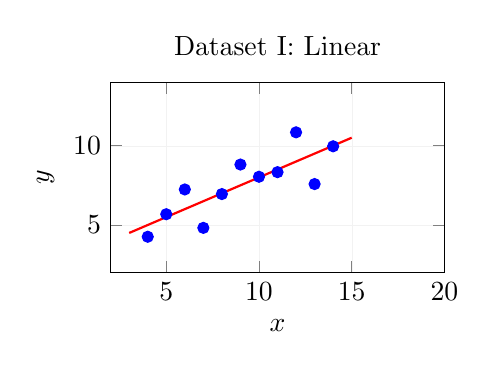
\begin{tikzpicture}
\begin{axis}[
    width=0.48\textwidth, height=4cm, title={Dataset I: Linear},
    xmin=2, xmax=20, ymin=2, ymax=14, xlabel={$x$}, ylabel={$y$},
    grid=both, grid style={line width=.1pt, color=gray!10}
]
    \addplot[only marks, mark=*, blue] coordinates {
        (10,8.04) (8,6.95) (13,7.58) (9,8.81) (11,8.33) 
        (14,9.96) (6,7.24) (4,4.26) (12,10.84) (7,4.82) (5,5.68)
    };
    \addplot[red, domain=3:15, thick] {3 + 0.5*x};
\end{axis}
\end{tikzpicture}
\hfill
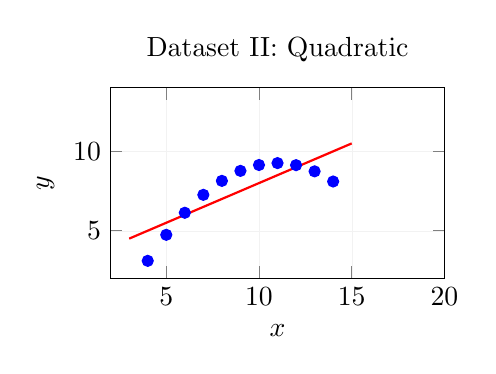
\begin{tikzpicture}
\begin{axis}[
    width=0.48\textwidth, height=4cm, title={Dataset II: Quadratic},
    xmin=2, xmax=20, ymin=2, ymax=14, xlabel={$x$}, ylabel={$y$},
    grid=both, grid style={line width=.1pt, color=gray!10}
]
    \addplot[only marks, mark=*, blue] coordinates {
        (10,9.14) (8,8.14) (13,8.74) (9,8.77) (11,9.26) 
        (14,8.10) (6,6.13) (4,3.10) (12,9.13) (7,7.26) (5,4.74)
    };
    \addplot[red, domain=3:15, thick] {3 + 0.5*x};
\end{axis}
\end{tikzpicture}

\vspace{0.3cm}

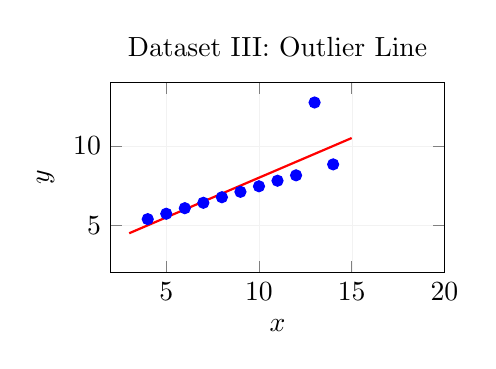
\begin{tikzpicture}
\begin{axis}[
    width=0.48\textwidth, height=4cm, title={Dataset III: Outlier Line},
    xmin=2, xmax=20, ymin=2, ymax=14, xlabel={$x$}, ylabel={$y$},
    grid=both, grid style={line width=.1pt, color=gray!10}
]
    \addplot[only marks, mark=*, blue] coordinates {
        (10,7.46) (8,6.77) (13,12.74) (9,7.11) (11,7.81) 
        (14,8.84) (6,6.08) (4,5.39) (12,8.15) (7,6.42) (5,5.73)
    };
    \addplot[red, domain=3:15, thick] {3 + 0.5*x};
\end{axis}
\end{tikzpicture}
\hfill
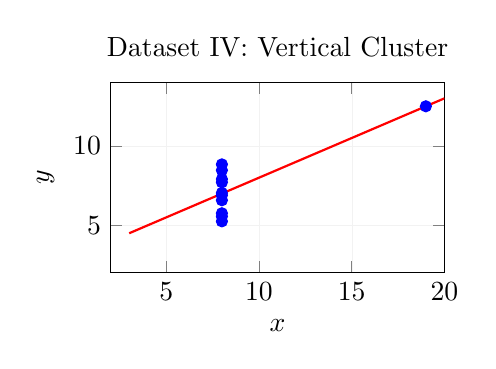
\begin{tikzpicture}
\begin{axis}[
    width=0.48\textwidth, height=4cm, title={Dataset IV: Vertical Cluster},
    xmin=2, xmax=20, ymin=2, ymax=14, xlabel={$x$}, ylabel={$y$},
    grid=both, grid style={line width=.1pt, color=gray!10}
]
    \addplot[only marks, mark=*, blue] coordinates {
        (8,6.58) (8,5.76) (8,7.71) (8,8.84) (8,8.47) 
        (8,7.04) (8,5.25) (19,12.50) (8,5.56) (8,7.91) (8,6.89)
    };
    \addplot[red, domain=3:20, thick] {3 + 0.5*x};
\end{axis}
\end{tikzpicture}
\end{center}

\vspace{0.2cm}
\noindent \textbf{The Datasaurus Dozen:} This concept scales up significantly via \textit{simulated annealing} (a derivative-free optimization method). Optimization models shift thousands of coordinates to match arbitrary shapes (such as a geometric star, circles, or a Tyrannosaurus Rex) while keeping the underlying means, variances, and correlations locked to perfectly identical values.

\subsubsection*{2. One-Dimensional Blind Spots: Box Plots vs. Violin Plots}

The loss of critical context via global summaries is equally prevalent in one-dimensional data profiles. Below is a structural demonstration showing why a traditional Box Plot can obscure structural data variations that a Violin Plot natively exposes:

\begin{center}
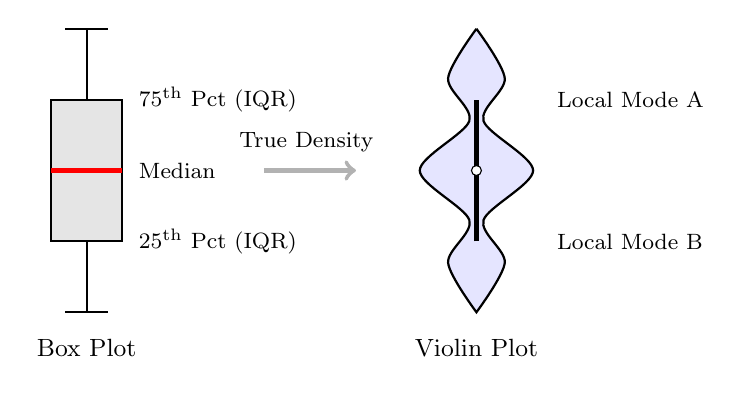
\begin{tikzpicture}[scale=0.9]
    % Left side: Box plot architecture
    \draw[thick] (1,0) -- (1,4); 
    \draw[thick] (0.7,0) -- (1.3,0); 
    \draw[thick] (0.7,4) -- (1.3,4); 
    \draw[fill=gray!20, thick] (0.5,1) rectangle (1.5,3); 
    \draw[ultra thick, red] (0.5,2) -- (1.5,2); 
    \node at (1, -0.5) {\small Box Plot};
    \node[anchor=west] at (1.6,3) {\footnotesize $75^{\text{th}}$ Pct (IQR)};
    \node[anchor=west] at (1.6,2) {\footnotesize Median};
    \node[anchor=west] at (1.6,1) {\footnotesize $25^{\text{th}}$ Pct (IQR)};

    % Arrow showing hidden structural data
    \draw[->, ultra thick, gray!60] (3.5,2) -- (4.8,2);
    \node at (4.1,2.4) {\footnotesize True Density};

    % Right side: Violin plot showing hidden Bimodal distribution
    \begin{scope}[shift={(6.5,2)}]
        \draw[thick, fill=blue!10] plot[smooth, tension=0.5] coordinates {
            (0,2) (-0.4,1.3) (-0.1,0.7) (-0.8,0) (-0.1,-0.7) (-0.4,-1.3) (0,-2)
        } -- plot[smooth, tension=0.5] coordinates {
            (0,-2) (0.4,-1.3) (0.1,-0.7) (0.8,0) (0.1,0.7) (0.4,1.3) (0,2)
        };
        \draw[ultra thick, black] (0,-1) -- (0,1);
        \draw[fill=white] (0,0) circle (2pt);
        \node at (0, -2.5) {\small Violin Plot};
        \node[anchor=west] at (1.0,1) {\footnotesize Local Mode A};
        \node[anchor=west] at (1.0,-1) {\footnotesize Local Mode B};
    \end{scope}
\end{tikzpicture}
\end{center}

\begin{itemize}
    \item \textbf{Box Plots:} Map a distribution using basic static quantiles, highlighting the median and the Interquartile Range ($\text{IQR}$). However, completely divergent probability density functions (e.g., a uniform distribution, a highly peaked unimodal distribution, or a multi-modal mixture) can map to the exact same box coordinates.
    \item \textbf{Violin Plots:} Mitigate this blind spot by overlaying a continuous \textbf{Kernel Density Estimate (KDE)} symmetrically along the axis. As shown above, it easily captures multi-modal valleys and spikes that summaries smooth over.
\end{itemize}

\begin{tcolorbox}[colback=red!5!white, colframe=red!75!black, title=Methodological Takeaway]
Numerical summaries should only be treated as auxiliary metrics. Data visualization is a mandatory prerequisite for statistical modeling to prevent the misinterpretation of underlying distribution structures.
\end{tcolorbox}

\section*{Bayes' Rule}

\begin{quote}
``Bayes's theorem is to the theory of probability what Pythagoras's theorem is to geometry.'' \\
\hfill --- Sir Harold Jeffreys, 1973
\end{quote}

Bayesian inference treats probability as a representation of ``degrees of certainty'' or belief. It provides a formal framework for updating these beliefs dynamically as new empirical sample data is gathered.

\subsubsection*{1. Mathematical Formulation}
Let $H$ denote an unobserved (hidden) hypothesis, and let $Y$ represent observed data evidence. Bayes' rule computes the conditional probability distribution over the unknown parameters given the observed realization $Y = y$:

\begin{equation}
    p(H = h \mid Y = y) = \frac{p(H = h) p(Y = y \mid H = h)}{p(Y = y)}
\end{equation}

This formula is derived directly from the product rule of probability:
\begin{equation}
    p(h \mid y)p(y) = p(h, y) = p(h)p(y \mid h)
\end{equation}

\noindent We can break down the structural roles of each term:
\begin{itemize}
    \item \textbf{Prior Distribution $p(H)$:} The foundational belief state regarding the parameters before evaluating current data.
    \item \textbf{Likelihood Function $p(Y = y \mid H = h)$:} The probability of observing the data point $y$ given a specific parameter state $h$. Regarded as a function of $h$, the likelihood is \textit{not} a true probability distribution and does not integrate to 1.
    \item \textbf{Marginal Likelihood $p(Y = y)$:} Also called the \textbf{Evidence}, this term serves as the normalization constant computed by marginalizing across the entire hypothesis space $\mathcal{H}$:
    \begin{equation}
        \label{eq:marginal_likelihood}
        p(Y = y) = \sum_{h' \in \mathcal{H}} p(H = h') p(Y = y \mid H = h')
    \end{equation}
    \item \textbf{Posterior Distribution $p(H = h \mid Y = y)$:} The updated belief mapping after observing data.
\end{itemize}

Since the denominator $p(Y=y)$ is constant with respect to $H$, Bayes' rule is frequently expressed in its unnormalized proportional form:
\begin{equation}
    \text{posterior} \propto \text{prior} \times \text{likelihood}
\end{equation}

\subsubsection*{2. Numerical Application: Diagnostic Testing \& The Base Rate Fallacy}
To understand the impact of the prior baseline, consider a binary classification scenario tracking a disease state ($H \in \{0,1\}$) via an observed diagnostic marker ($Y \in \{0,1\}$). Let the testing parameters be defined as:
\begin{align*}
    \text{Sensitivity (True Positive Rate, TPR)} &= p(Y=1 \mid H=1) = 0.875 \\
    \text{Specificity (True Negative Rate, TNR)} &= p(Y=0 \mid H=0) = 0.975 \\
    \text{False Positive Rate (FPR)} &= 1 - \text{TNR} = 0.025 
\end{align*}

\noindent \textbf{Case 1: High Prevalence Area (NYC Spring 2020)} \\
Assuming a prior prevalence rate of 10\% ($p(H=1) = 0.10$), the posterior probability of infection given a positive test ($Y=1$) is evaluated using Equation \ref{eq:marginal_likelihood}:
\begin{align}
    p(H=1 \mid Y=1) &= \frac{\text{TPR} \times p(H=1)}{\text{TPR} \times p(H=1) + \text{FPR} \times p(H=0)} \\
    &= \frac{0.875 \times 0.1}{(0.875 \times 0.1) + (0.025 \times 0.9)} = \frac{0.0875}{0.11} \approx \mathbf{0.795}
\end{align}

\noindent \textbf{Case 2: Low Prevalence Area (Base Rate Fallacy Anomaly)} \\
If the prior disease baseline falls to 1\% ($p(H=1) = 0.01$), recalculating under identical test accuracy yields:
\begin{equation}
    p(H=1 \mid Y=1) = \frac{0.875 \times 0.01}{(0.875 \times 0.01) + (0.025 \times 0.99)} = \frac{0.00875}{0.0335} \approx \mathbf{0.260}
\end{equation}

\begin{tcolorbox}[colback=red!5!white, colframe=red!75!black, title=The Intuitive Disconnect]
Even with a highly accurate diagnostic tool ($97.5\%$ specificity), testing positive in a low-prevalence population yields only a \textbf{$26\%$} chance of actual infection. This occurs because the rare baseline rate causes the sheer volume of absolute false positives to mathematically dwarf the true positives.
\end{tcolorbox}

\subsubsection*{3. Structural Population Tree (1\% Base Rate Context)}
The structural division of outcomes across an empirical sample pool of 100,000 individuals clarifies the dominance of false positives:

\begin{center}
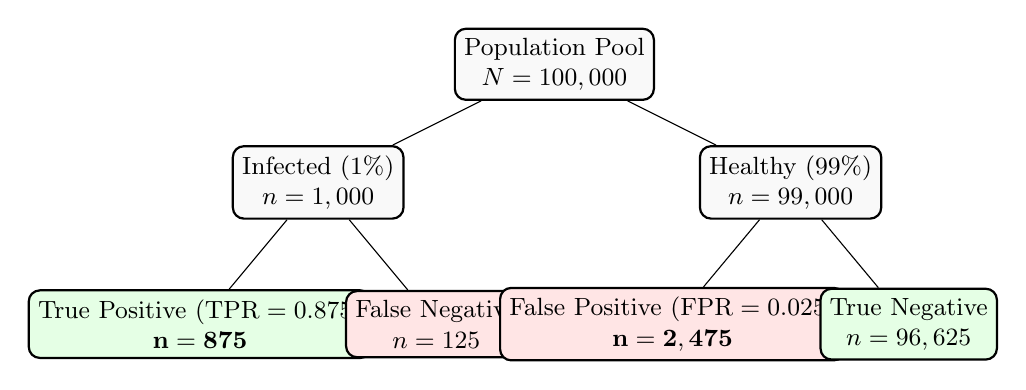
\begin{tikzpicture}[
    level 1/.style={sibling distance=6cm, level distance=1.5cm},
    level 2/.style={sibling distance=3cm, level distance=1.8cm},
    every node/.style={transform shape, align=center, draw, thick, rounded corners, fill=gray!5, font=\small}
]
    % Root
    \node {Population Pool \\ $N = 100,000$}
        child { node {Infected ($1\%$) \\ $n = 1,000$} 
            child { node [fill=green!10] {True Positive ($\text{TPR}=0.875$) \\ $\mathbf{n = 875}$} }
            child { node [fill=red!10] {False Negative \\ $n = 125$} }
        }
        child { node {Healthy ($99\%$) \\ $n = 99,000$} 
            child { node [fill=red!10] {False Positive ($\text{FPR}=0.025$) \\ $\mathbf{n = 2,475}$} }
            child { node [fill=green!10] {True Negative \\ $n = 96,625$} }
        };
\end{tikzpicture}
\end{center}

\begin{equation}
    p(H=1 \mid Y=1) = \frac{\text{True Positives}}{\text{True Positives} + \text{False Positives}} = \frac{875}{875 + 2475} = \frac{875}{3350} \approx 0.260
\end{equation}

\section*{The Law of Total Probability and Bayes' Theorem}

\subsubsection*{1. The Law of Total Probability}
The \textbf{Law of Total Probability} provides a way to calculate the overall probability of an event $A$ when it can happen under several mutually exclusive and exhaustive scenarios $B_1, B_2, \dots, B_n$:
\begin{equation}
    p(A) = \sum_{i=1}^{n} p(A \mid B_i) p(B_i)
\end{equation}

\subsubsection*{2. Bayes' Theorem}
Once event $A$ has actually occurred, \textbf{Bayes' Theorem} allows us to reverse the conditional dependency to find the probability that a specific scenario $B_k$ was the underlying cause:
\begin{equation}
    p(B_k \mid A) = \frac{p(A \mid B_k) p(B_k)}{p(A)} = \frac{p(A \mid B_k) p(B_k)}{\sum_{i=1}^{n} p(A \mid B_i) p(B_i)}
\end{equation}

\subsubsection*{3. A Simple Numerical Example}
Consider predicting whether you will be late to work ($L$) based on the morning weather, which can either be Rainy ($R$) or Sunny ($S$). 

\noindent Suppose we have the following historical baseline probabilities (priors) and conditional likelihoods:
\begin{itemize}
    \item \textbf{Probability of rain:} $p(R) = 0.20$
    \item \textbf{Probability of sun:} $p(S) = 0.80$
    \item \textbf{Probability of being late if it rains:} $p(L \mid R) = 0.50$
    \item \textbf{Probability of being late if it is sunny:} $p(L \mid S) = 0.10$
\end{itemize}

\vspace{0.2cm}
\noindent \textbf{Step 1: Find the Total Probability of Being Late} \\
Using the Law of Total Probability, we aggregate your chances of being late across both possible weather scenarios:
\begin{align}
    p(L) &= p(L \mid R)p(R) + p(L \mid S)p(S) \\
    &= (0.50 \times 0.20) + (0.10 \times 0.80) \\
    &= 0.10 + 0.08 = \mathbf{0.18}
\end{align}
This means there is an overall $18\%$ chance that you will be late on any given day.

\vspace{0.2cm}
\noindent \textbf{Step 2: Apply Bayes' Theorem to Reverse the Conditions} \\
Now suppose you walk into the office late ($L$). Given only this information, what is the probability that it is currently raining outside? We use Bayes' Theorem to update our belief:
\begin{equation}
    p(R \mid L) = \frac{p(L \mid R)p(R)}{p(L)} = \frac{0.50 \times 0.20}{0.18} = \frac{0.10}{0.18} \approx \mathbf{0.556}
\end{equation}

\begin{tcolorbox}[colback=green!5!white, colframe=green!60!black, title=Intuitive Takeaway]
Even though it only rains $20\%$ of the time normally, knowing that you arrived late causes the probability of rain to jump to $55.6\%$. This happens because being late is five times more likely when it rains ($50\%$) than when it is sunny ($10\%$).
\end{tcolorbox}

\section*{The Monty Hall Problem}

The \textbf{Monty Hall Problem} is a famous probability puzzle based on the American television game show \textit{Let's Make a Deal}. It highlights how human intuition frequently fails when evaluating conditional probabilities.

\subsubsection*{1. The Setup}
Suppose you are on a game show, and you are given the choice of three doors:
\begin{itemize}
    \item Behind one door is a car (the prize you want).
    \item Behind the other two doors are goats (booby prizes).
\end{itemize}
The game proceeds in three steps:
\begin{enumerate}
    \item You pick a door—say, \textbf{Door 1}.
    \item The host, Monty Hall, who knows exactly what is behind every door, opens another door—say, \textbf{Door 3}—to reveal a goat.
    \item Monty then turns to you and asks: ``Do you want to switch to Door 2?''
\end{enumerate}
Is it to your advantage to switch your choice?

\subsubsection*{2. Bayesian Analysis}
Let $C_i$ denote the event that the car is behind Door $i$ (where $i \in \{1, 2, 3\}$). Before any doors are opened, your prior probability of winning is uniformly distributed:
\begin{equation}
    p(C_1) = p(C_2) = p(C_3) = \frac{1}{3}
\end{equation}

\noindent Assume you have chosen \textbf{Door 1}. Let $M_3$ represent the event that Monty opens \textbf{Door 3} to show a goat. We evaluate the conditional likelihoods of Monty's action under each hypothesis:
\begin{itemize}
    \item \textbf{If the car is behind Door 1 ($C_1$):} Monty can open either Door 2 or Door 3. Assuming he chooses randomly:
    \begin{equation}
        p(M_3 \mid C_1) = \frac{1}{2}
    \end{equation}
    \item \textbf{If the car is behind Door 2 ($C_2$):} Since you picked Door 1 and the car is behind Door 2, Monty is forced to open Door 3:
    \begin{equation}
        p(M_3 \mid C_2) = 1
    \end{equation}
    \item \textbf{If the car is behind Door 3 ($C_3$):} Monty cannot open a door that contains the car:
    \begin{equation}
        p(M_3 \mid C_3) = 0
    \end{equation}
\end{itemize}

\vspace{0.2cm}
\noindent \textbf{Step 1: Compute Total Probability of the Host's Action} \\
Using the Law of Total Probability, the overall probability of Monty opening Door 3 is:
\begin{align}
    p(M_3) &= p(M_3 \mid C_1)p(C_1) + p(M_3 \mid C_2)p(C_2) + p(M_3 \mid C_3)p(C_3) \\
    &= \left(\frac{1}{2} \times \frac{1}{3}\right) + \left(1 \times \frac{1}{3}\right) + \left(0 \times \frac{1}{3}\right) \\
    &= \frac{1}{6} + \frac{1}{3} + 0 = \mathbf{\frac{1}{2}}
\end{align}

\noindent \textbf{Step 2: Compute Posteriors Using Bayes' Theorem} \\
Now we calculate the posterior probability of winning if you stick with your original choice versus if you switch.

\noindent \textbf{Probability of winning if you STAY (Door 1):}
\begin{equation}
    p(C_1 \mid M_3) = \frac{p(M_3 \mid C_1)p(C_1)}{p(M_3)} = \frac{\frac{1}{2} \times \frac{1}{3}}{\frac{1}{2}} = \mathbf{\frac{1}{3}}
\end{equation}

\noindent \textbf{Probability of winning if you SWITCH (Door 2):}
\begin{equation}
    p(C_2 \mid M_3) = \frac{p(M_3 \mid C_2)p(C_2)}{p(M_3)} = \frac{1 \times \frac{1}{3}}{\frac{1}{2}} = \mathbf{\frac{2}{3}}
\end{equation}
The math proves that switching doubles your chances of winning from $\frac{1}{3}$ to $\frac{2}{3}$.

\subsubsection*{3. The Simple Intuition}
If the math feels confusing, think about the initial choice. When you first select Door 1, there is a $\frac{1}{3}$ chance you chose the car correctly, and a $\frac{2}{3}$ chance that the car is hidden in the group consisting of \textbf{\{Door 2, Door 3\}}.

Monty's action does not change the fact that the two unchosen doors combined have a $\frac{2}{3}$ probability of holding the car. However, by opening Door 3 and filtering out a goat, Monty effectively concentrates all of that $\frac{2}{3}$ probability directly into **Door 2**. 

\begin{tcolorbox}[colback=green!5!white, colframe=green!60!black, title=Intuitive Takeaway]
You should always switch. Sticking with your door means you only win if you were right on your very first guess ($\frac{1}{3}$ chance). Switching means you win every single time your initial guess was wrong ($\frac{2}{3}$ chance), because Monty is guaranteed to clear away the other wrong option for you.
\end{tcolorbox}

\section*{Bernoulli and Binomial Distributions}

The simplest discrete probability landscapes are built around binary events where outcomes are strictly categorical and dichotomous (e.g., success/failure, heads/tails).

\subsubsection*{1. The Bernoulli Distribution}
Consider a single random trial yielding an outcome $Y \in \{0, 1\}$, where the probability of success is parameterized by $\theta \in [0,1]$. We denote this distribution as $Y \sim \text{Ber}(\theta)$. The structural assignment maps to:
\begin{equation}
    p(Y=1) = \theta \quad \text{and} \quad p(Y=0) = 1 - \theta
\end{equation}

\noindent The conditional probability mass function (PMF) can be written compactly using conditional switching exponents:
\begin{equation}
    \text{Ber}(y \mid \theta) \triangleq \theta^y (1 - \theta)^{1-y}
\end{equation}
When evaluating $y=1$, the term $(1-\theta)^0$ drops out; conversely, evaluating $y=0$ forces $\theta^0$ to collapse to unity, natively reproducing the foundational binary mappings.

\subsubsection*{2. The Binomial Distribution}
The \textbf{Binomial distribution} generalizes the Bernoulli profile to a sequence of $N$ independent and identically distributed (\textit{i.i.d.}) trials. Let $y_n \sim \text{Ber}(\cdot \mid \theta)$ for $n=1 \dots N$. If we define $s$ as the cumulative sum of successful trials observed ($s \triangleq \sum_{n=1}^N \mathbb{I}(y_n = 1)$), then $s \sim \text{Bin}(N, \theta)$. 

The PMF scales based on structural configurations:
\begin{equation}
    \text{Bin}(s \mid N, \theta) \triangleq \binom{N}{s} \theta^s (1 - \theta)^{N-s}
\end{equation}
The algebraic component $\binom{N}{s}$ represents the \textbf{binomial coefficient}, defining the total permutations available to seat $s$ successes across $N$ open temporal slots:
\begin{equation}
    \binom{N}{s} \triangleq \frac{N!}{(N - s)!s!}
\end{equation}
If the cumulative sequence restriction drops to $N=1$, the Binomial PMF simplifies directly back to a standard baseline Bernoulli trial.

\subsubsection*{3. Parametric PMF Geometry Comparisons ($N=5$)}
The physical structure of a Binomial distribution shifts distinctly based on changes made to the internal success parameter $\theta$. Below are discrete PMF mappings showing a fair system vs. a highly skewed variant:

\begin{center}
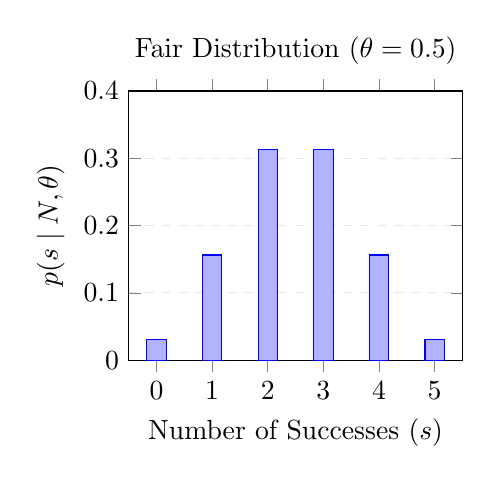
\begin{tikzpicture}
\begin{axis}[
    width=0.48\textwidth, height=5cm,
    title={Fair Distribution ($\theta = 0.5$)},
    xlabel={Number of Successes ($s$)}, ylabel={$p(s \mid N, \theta)$},
    xmin=-0.5, xmax=5.5, ymin=0, ymax=0.4,
    xtick={0,1,2,3,4,5},
    ybar, bar width=7pt,
    ymajorgrids=true, grid style={dashed, gray!20}
]
    \addplot[draw=blue, fill=blue!30] coordinates {
        (0,0.03125) (1,0.15625) (2,0.31250) (3,0.31250) (4,0.15625) (5,0.03125)
    };
\end{axis}
\end{tikzpicture}
\hfill
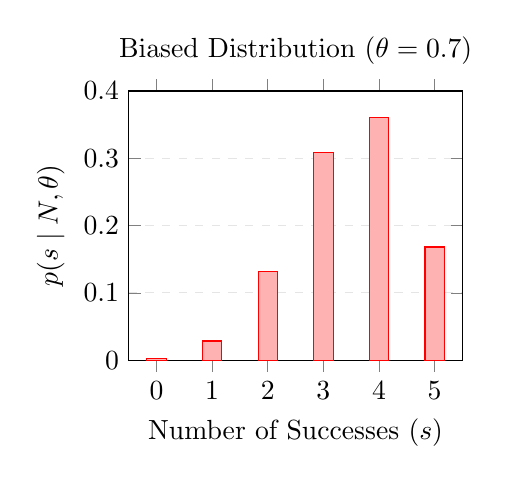
\begin{tikzpicture}
\begin{axis}[
    width=0.48\textwidth, height=5cm,
    title={Biased Distribution ($\theta = 0.7$)},
    xlabel={Number of Successes ($s$)}, ylabel={$p(s \mid N, \theta)$},
    xmin=-0.5, xmax=5.5, ymin=0, ymax=0.4,
    xtick={0,1,2,3,4,5},
    ybar, bar width=7pt,
    ymajorgrids=true, grid style={dashed, gray!20}
]
    \addplot[draw=red, fill=red!30] coordinates {
        (0,0.00243) (1,0.02835) (2,0.13230) (3,0.30870) (4,0.36015) (5,0.16807)
    };
\end{axis}
\end{tikzpicture}
\end{center}

\begin{tcolorbox}[colback=blue!5!white, colframe=blue!60!black, title=Analytical Insights]
As shown in the structural plots above:
\begin{itemize}
    \item When $\theta = 0.5$, the discrete mass profile displays perfect symmetry around the central expected median location ($\mu = N\theta = 2.5$).
    \item When $\theta = 0.7$, the distribution develops a heavy left skew, concentrating its primary probability density toward the upper bounds of the sampling range.
\end{itemize}
\end{tcolorbox}

\section*{The Sigmoid Function and Logistic Regression}

In binary classification tasks where $y \in \{0, 1\}$, a machine learning model must output a valid probability bounded strictly between $0$ and $1$. An unconstrained linear predictor function $f(x; \theta) = w^T x + b$ can output any real value on the interval $(-\infty, \infty)$. To transform this unconstrained value into a valid Bernoulli parameter space, we map it through a non-linear squeezing function.

\begin{equation}
    p(y=1 \mid x, \theta) = \text{Ber}(y \mid \sigma(f(x; \theta)))
\end{equation}

\noindent where $\sigma(a)$ represents the \textbf{sigmoid} (or logistic) function, defined analytically as:
\begin{equation}
    \sigma(a) \triangleq \frac{1}{1 + e^{-a}} = \frac{e^a}{1 + e^a}
\end{equation}

\subsubsection*{1. Deep Mathematical Characterization}

To understand why the sigmoid function serves as the bedrock of probabilistic machine learning models, we analyze its fundamental mathematical properties:

\begin{itemize}
    \item \textbf{Domain and Range:} The function maps the unconstrained real number line smoothly to an open probability interval:
    \begin{equation}
        \sigma(a): \mathbb{R} \to (0, 1)
    \end{equation}
    
    \item \textbf{Continuity and Differentiability:} The function is infinitely differentiable ($C^\infty$ continuous). This is critical for optimization techniques like gradient descent. Conversely, the discrete \textbf{Heaviside step function}:
    \begin{equation}
        H(a) \triangleq \mathbb{I}(a > 0) = \begin{cases} 1 & \text{if } a > 0 \\ 0 & \text{if } a \le 0 \end{cases}
    \end{equation}
    has a step discontinuity at $a=0$. Its derivative is zero everywhere except at the origin, where it is undefined. This zero-gradient property prevents models using $H(a)$ from learning via gradient-based optimization.
    
    \item \textbf{First Derivative (Local Gradient):} The derivative can be expressed entirely in terms of the function's output values, removing the need for costly exponential operations during backpropagation:
    \begin{align}
        \frac{d}{da}\sigma(a) &= \frac{d}{da} (1 + e^{-a})^{-1} = -(1 + e^{-a})^{-2} \cdot (-e^{-a}) \\
        &= \frac{e^{-a}}{(1 + e^{-a})^2} = \left(\frac{1}{1 + e^{-a}}\right)\left(\frac{e^{-a}}{1 + e^{-a}}\right) \\
        &= \sigma(a)\left(1 - \sigma(a)\right)
    \end{align}
    The maximum rate of change occurs exactly at the center ($a=0$), where $\sigma'(0) = 0.5 \times (1 - 0.5) = 0.25$. As $a \to \pm\infty$, the gradient approaches $0$, a phenomenon known as \textit{gradient saturation}.

    \item \textbf{Inflection Point and Symmetry:} The function possesses rotational symmetry around its central coordinate $(0, 0.5)$, satisfying $\sigma(-a) = 1 - \sigma(a)$. We locate its point of inflection by calculating the second derivative via the product rule:
    \begin{align}
        \sigma''(a) &= \frac{d}{da} \left[ \sigma(a)(1 - \sigma(a)) \right] \\
        &= \sigma'(a)(1 - \sigma(a)) + \sigma(a)(-\sigma'(a)) \\
        &= \sigma'(a)\left(1 - 2\sigma(a)\right)
    \end{align}
    Setting $\sigma''(a) = 0$ to look for changes in concavity, since the first derivative $\sigma'(a)$ is strictly positive for all real inputs, the second term must equal zero:
    \begin{equation}
        1 - 2\sigma(a) = 0 \implies \sigma(a) = 0.5 \implies a = 0
    \end{equation}
    Thus, $(0, 0.5)$ is the exact inflection point where the curve switches from convex ($\sigma''(a) > 0$ for $a < 0$) to concave ($\sigma''(a) < 0$ for $a > 0$).
\end{itemize}

\subsubsection*{2. Geometric Function Profiles}
The plots below contrast the smooth, differentiable transition of the sigmoid function against the abrupt threshold jump of the Heaviside step function:

\begin{center}
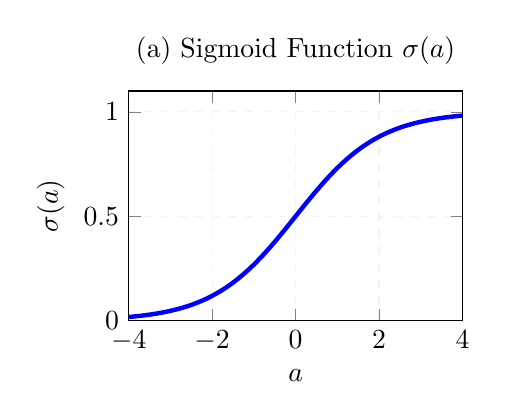
\begin{tikzpicture}
\begin{axis}[
    width=0.48\textwidth, height=4.5cm,
    title={(a) Sigmoid Function $\sigma(a)$},
    xlabel={$a$}, ylabel={$\sigma(a)$},
    xmin=-4, xmax=4, ymin=0, ymax=1.1,
    grid=both, grid style={dashed, gray!10}
]
    \addplot[blue, ultra thick, domain=-4:4, samples=100] {1 / (1 + exp(-x))};
\end{axis}
\end{tikzpicture}
\hfill
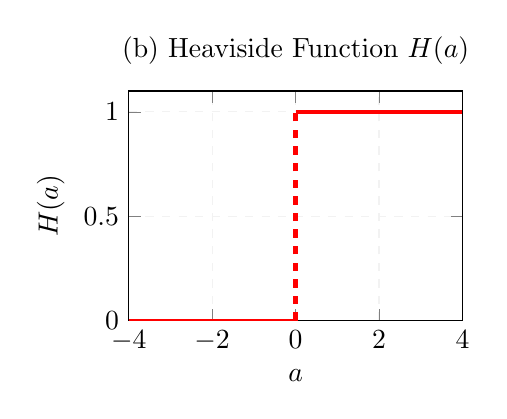
\begin{tikzpicture}
\begin{axis}[
    width=0.48\textwidth, height=4.5cm,
    title={(b) Heaviside Function $H(a)$},
    xlabel={$a$}, ylabel={$H(a)$},
    xmin=-4, xmax=4, ymin=0, ymax=1.1,
    grid=both, grid style={dashed, gray!10}
]
    \addplot[red, ultra thick, domain=-4:0, samples=2] {0};
    \addplot[red, ultra thick, domain=0:4, samples=2] {1};
    \draw[red, ultra thick, dashed] (axis cs:0,0) -- (axis cs:0,1);
\end{axis}
\end{tikzpicture}
\end{center}

\subsubsection*{3. Binary Logistic Regression \& Simple Numerical Example}
\textbf{Binary logistic regression} applies this framework to linear classification. It calculates a weighted linear score from input features, then pipes that score directly into the sigmoid operator:
\begin{equation}
    p(y = 1 \mid x; \theta) = \sigma(w^T x + b) = \frac{1}{1 + e^{-(w^T x + b)}}
\end{equation}

\noindent \textbf{The Decision Boundary:} The geometric separating boundary matches the coordinates where the model is completely unsure ($50\%$ probability):
\begin{equation}
    p(y = 1 \mid x^*; \theta) = 0.5 \iff w^T x^* + b = 0
\end{equation}

\noindent \textbf{Intuitive Numerical Example:} \\
Imagine predicting whether a student passes an exam ($y=1$) or fails ($y=0$) based on a single feature: study duration ($x$, measured in hours). Let's assume a trained model yields the parameters $w = 2.0$ and intercept $b = -4.0$. The internal unconstrained score equation expands to $a = 2x - 4$.

We evaluate the probability of passing for three separate students:
\begin{itemize}
    \item \textbf{Student A (Low Input): $x = 1.0$ hour}
    \begin{align}
        a &= 2(1.0) - 4 = -2.0 \\
        p(y=1 \mid x=1.0) &= \sigma(-2.0) = \frac{1}{1 + e^{-(-2.0)}} = \frac{1}{1 + e^2} \approx \frac{1}{1 + 7.389} \approx \mathbf{0.119}
    \end{align}
    There is an $11.9\%$ chance this student passes.
    
    \item \textbf{Student B (Boundary Input): $x = 2.0$ hours}
    \begin{align}
        a &= 2(2.0) - 4 = 0.0 \\
        p(y=1 \mid x=2.0) &= \sigma(0.0) = \frac{1}{1 + e^{0}} = \frac{1}{1 + 1} = \mathbf{0.500}
    \end{align}
    At exactly $2.0$ hours of studying, the model outputs a $50\%$ pass chance. This represents the classification decision boundary.
    
    \item \textbf{Student C (High Input): $x = 3.5$ hours}
    \begin{align}
        a &= 2(3.5) - 4 = 3.0 \\
        p(y=1 \mid x=3.5) &= \sigma(3.0) = \frac{1}{1 + e^{-3.0}} \approx \frac{1}{1 + 0.0498} \approx \mathbf{0.953}
    \end{align}
    There is a $95.3\%$ chance this student passes.
\end{itemize}

\subsubsection*{4. Empirical Simulation: 1D Logistic Regression Classification}
Below is a visual layout of this classification framework. Notice how the continuous logistic line transitions smoothly between the binary labels, avoiding out-of-bounds extrapolations ($>1$ or $<0$) that happen if you try to fit a standard linear regression line to categorical data:

\begin{center}
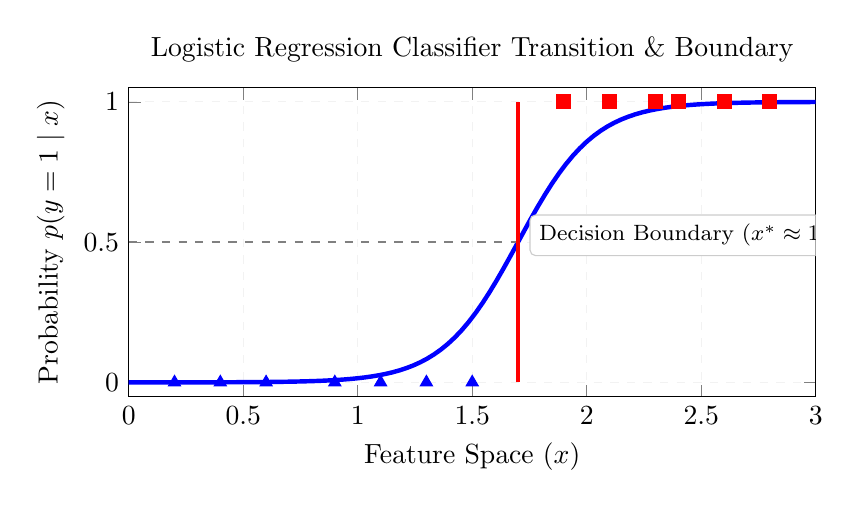
\begin{tikzpicture}
\begin{axis}[
    width=0.85\textwidth, height=5.5cm,
    title={Logistic Regression Classifier Transition \& Boundary},
    xlabel={Feature Space ($x$)}, ylabel={Probability $p(y=1 \mid x)$},
    xmin=0, xmax=3, ymin=-0.05, ymax=1.05,
    grid=both, grid style={dashed, gray!10}
]
    % Sigmoid function fit
    \addplot[blue, ultra thick, domain=0:3, samples=100] {1 / (1 + exp(-6*(x - 1.7)))};
    
    % Data classes
    \addplot[only marks, mark=triangle*, blue, mark size=2.5pt] coordinates {
        (0.2,0) (0.4,0) (0.6,0) (0.9,0) (1.1,0) (1.3,0) (1.5,0)
    };
    \addplot[only marks, mark=square*, red, mark size=2.5pt] coordinates {
        (1.9,1) (2.1,1) (2.3,1) (2.4,1) (2.6,1) (2.8,1)
    };
    
    % Boundary indicators
    \draw[dashed, black!50, line width=0.8pt] (axis cs:0,0.5) -- (axis cs:1.7,0.5);
    \draw[red, line width=1.2pt] (axis cs:1.7,0) -- (axis cs:1.7,1);
    
    \node[anchor=south west, fill=white, draw=gray!40, rounded corners=2pt, font=\footnotesize] 
        at (axis cs:1.75,0.45) {Decision Boundary ($x^* \approx 1.7$)};
\end{axis}
\end{tikzpicture}
\end{center}

\begin{tcolorbox}[colback=blue!5!white, colframe=blue!60!black, title=Modeling Intuition]
As the feature coordinate $x$ increases and moves rightward from the decision boundary marker, the log-odds increase proportionally, causing the classifier to asymptotically approach a probability of $1.0$, signaling high certainty in a positive class assignment.
\end{tcolorbox}

\section*{The Soft Step and the Logit Framework}

To fully utilize logistic regression and modern neural networks, we must understand how the sigmoid function acts as a smooth surrogate for discrete choices, and how its mathematical inverse—the logit—bridges raw model predictions with true probabilities.

\subsubsection*{1. Why Sigmoid is a ``Softer'' Heaviside Function}
The Heaviside step function $H(a)$ represents a rigid, deterministic rule: if an input score is greater than zero, it instantly jumps to a $1$; otherwise, it is $0$. There is no middle ground, no concept of uncertainty, and crucially, no gradient to guide learning.

The sigmoid function $\sigma(a)$ introduces a continuous, probabilistic transition. We can explicitly formalize this relationship by introducing a positive scaling parameter $k > 0$ (often called the \textbf{gain} or \textbf{inverse temperature}) to control the steepness of the curve:
\begin{equation}
    \sigma_k(a) \triangleq \frac{1}{1 + e^{-ka}}
\end{equation}

By analyzing the behavior of $\sigma_k(a)$ as $k$ varies, we can see exactly how it modulates ``softness'':
\begin{itemize}
    \item \textbf{When $k \to 0$ (Extreme Softness):} The curve flattens out completely. The exponential term $e^0 \to 1$, forcing the output to a uniform state of maximum uncertainty: $\sigma(a) \to 0.5$ for all inputs.
    \item \textbf{When $k = 1$:} We recover the standard, smooth activation curve used in baseline logistic regression.
    \item \textbf{When $k \to \infty$ (Hardening):} The transition becomes infinitely steep. If $a > 0$, then $-ka \to -\infty$, meaning $e^{-ka} \to 0$, causing $\sigma_k(a) \to 1$. If $a < 0$, then $-ka \to \infty$, meaning $e^{-ka} \to \infty$, causing $\sigma_k(a) \to 0$. 
\end{itemize}

Mathematically, the standard Heaviside function is simply the limiting case of a scaled sigmoid function:
\begin{equation}
    \lim_{k \to \infty} \sigma_k(a) = H(a) \quad (\text{for } a \neq 0)
\end{equation}

By using the standard sigmoid ($k=1$), we are using a regularized, ``softened'' step function that permits small mistakes during training, preserves non-zero local gradients, and provides a continuous measure of classification confidence rather than a harsh binary verdict.

\subsubsection*{2. The Logit Function and ``Logits''}
In machine learning literature, you will constantly hear the term \textbf{logits}. To understand what they are, we must look at the mathematical inverse of the sigmoid function, known as the \textbf{logit function}.

If the sigmoid function maps an unconstrained score $a \in (-\infty, \infty)$ to a restricted probability $p \in (0, 1)$, the logit function reverses this operation:
\begin{equation}
    p = \frac{1}{1 + e^{-a}} \iff a = \text{logit}(p)
\end{equation}

We derive the algebraic form of the logit function by solving for $a$:
\begin{align}
    p(1 + e^{-a}) &= 1 \\
    1 + e^{-a} &= \frac{1}{p} \\
    e^{-a} &= \frac{1}{p} - 1 = \frac{1 - p}{p} \\
    e^a &= \frac{p}{1 - p}
\end{align}
Taking the natural logarithm of both sides yields the final definition:
\begin{equation}
    a = \text{logit}(p) \triangleq \log\left(\frac{p}{1 - p}\right)
\end{equation}

\noindent This equation reveals two fundamental concepts:
\begin{itemize}
    \item \textbf{The Odds Ratio:} The term $\frac{p}{1-p}$ represents the \textit{odds} of an event occurring (the probability of success divided by the probability of failure). For example, if a horse has a $75\%$ chance of winning ($p=0.75$), its odds of winning are $\frac{0.75}{0.25} = 3$, often stated as ``3 to 1''.
    \item \textbf{Log-Odds (Logits):} The logit function is simply the natural logarithm of the odds ratio. Therefore, \textbf{logits are log-odds}.
\end{itemize}

\subsubsection*{3. Practical Meaning in Machine Learning}
In deep learning and classification pipelines, a model calculates a raw, unconstrained real number for a given input via its final linear layer ($w^T x + b$). This raw score is called a **logit**. 

\begin{itemize}
    \item \textbf{Why models output logits natively:} Linear equations naturally generate values anywhere from $-\infty$ to $\infty$. Forcing a neural network's final layer to output numbers strictly between $0$ and $1$ without an activation function causes severe optimization instabilities.
    \item \textbf{The Mapping Pipeline:} The model computes a linear **logit** ($a \in \mathbb{R}$), and then the **sigmoid** function maps that logit to a squashed probability space ($p \in [0, 1]$).
\end{itemize}

\vspace{0.2cm}
\noindent \textbf{Quick Numerical Mapping Table:}
To build intuition for how these spaces interact, look at how raw logits translate to probabilities:
\begin{center}
\begin{tabular}{|c|c|c|l|}
\hline
\textbf{Logit ($a$)} & \textbf{Odds Ratio ($\frac{p}{1-p}$)} & \textbf{Probability ($p$)} & \textbf{Model Interpretation} \\ \hline
$-4.60$ & $e^{-4.60} \approx \frac{1}{100}$ & $\approx 0.01$ & Highly certain of negative class ($1\%$) \\ \hline
$-1.38$ & $e^{-1.38} \approx \frac{1}{4}$ & $\approx 0.20$ & Leaning negative class ($20\%$) \\ \hline
$\mathbf{0.00}$ & $e^{0} = 1$ & $\mathbf{0.50}$ & **Decision Boundary (Dead Unsure)** \\ \hline
$1.38$ & $e^{1.38} \approx 4$ & $\approx 0.80$ & Leaning positive class ($80\%$) \\ \hline
$4.60$ & $e^{4.60} \approx 100$ & $\approx 0.99$ & Highly certain of positive class ($99\%$) \\ \hline
\end{tabular}
\end{center}

\begin{tcolorbox}[colback=blue!5!white, colframe=blue!60!black, title=Core Structural Takeaway]
Logits and probabilities are two ways of looking at the same thing. A logit of $\mathbf{0}$ means the odds are $1:1$, which corresponds to a probability of $\mathbf{0.5}$. Every time a logit increases by $1$ unit linearly, the underlying odds of the event occurring scale multiplicatively by a factor of $e^1 \approx 2.718$.
\end{tcolorbox}

\section*{Binary Logistic Regression Fundamentals}

Binary logistic regression defines a conditional probability framework where a categorical target label $y \in \{0,1\}$ is modeled via a linear combination of input features mapped through a nonlinear activation function.

\subsubsection*{1. Mathematical Framework}
Rather than predicting the discrete label directly, the model estimates the parameter of a conditional Bernoulli distribution using a linear predictor $f(x; \theta) = w^T x + b$:
\begin{equation}
    p(y \mid x; \theta) = \text{Ber}\left(y \mid \sigma(w^T x + b)\right)
\end{equation}

\noindent Expanding this using the analytical definitions of the Bernoulli PMF and the logistic sigmoid yields:
\begin{equation}
    p(y = 1 \mid x; \theta) = \sigma(w^T x + b) = \frac{1}{1 + e^{-(w^T x + b)}}
\end{equation}

The \textbf{decision boundary} is characterized as the geometric locus of points $x^*$ where the model is perfectly ambivalent regarding the class assignment, corresponding to a posterior probability of exactly $0.5$:
\begin{equation}
    p(y = 1 \mid x^*; \theta) = 0.5 \iff w^T x^* + b = 0
\end{equation}
As an input feature vector $x$ moves away from this separating hyperplane, the absolute magnitude of the log-odds increases, causing the classifier's predictive confidence to asymptotically approach absolute certainty ($0$ or $1$).

\subsubsection*{2. Comparative Analysis: Logistic vs. Linear Regression}
Attempting to model a binary classification task using standard linear regression (Ordinary Least Squares) is known as creating a \textbf{Linear Probability Model (LPM)}. This approach introduces severe structural flaws. Below is a geometric visualization demonstrating why a linear model is mathematically invalid for bounded probability estimation:

\begin{center}
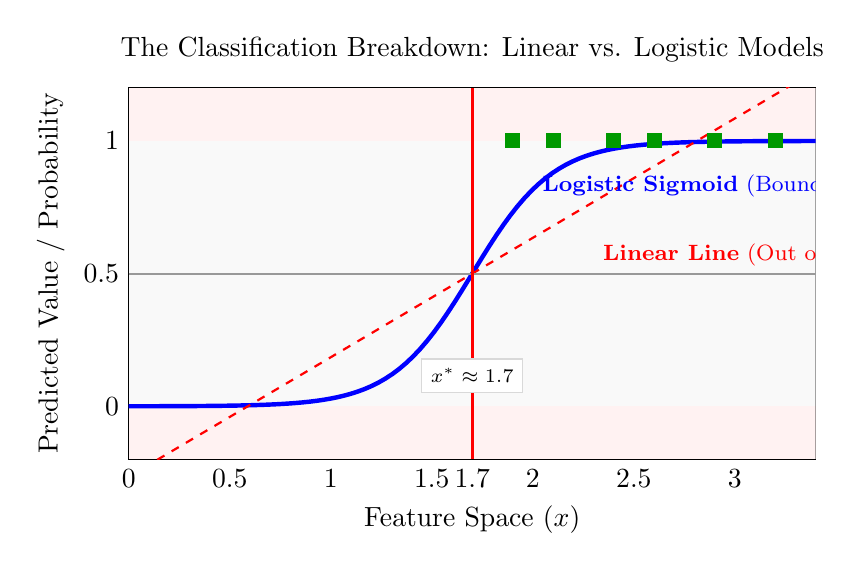
\begin{tikzpicture}
\begin{axis}[
    width=0.85\textwidth, height=6.3cm,
    title={The Classification Breakdown: Linear vs. Logistic Models},
    xlabel={Feature Space ($x$)}, ylabel={Predicted Value / Probability},
    xmin=0, xmax=3.4, ymin=-0.2, ymax=1.2,
    xtick={0, 0.5, 1.0, 1.5, 1.7, 2.0, 2.5, 3.0},
    grid=both, grid style={dashed, gray!10}
]
    % Bounded Probability Shading
    \fill[gray!5] (axis cs:0,0) rectangle (axis cs:3.4,1);
    
    % Out-of-bounds Shading
    \fill[red!5] (axis cs:0,-0.2) rectangle (axis cs:3.4,0);
    \fill[red!5] (axis cs:0,1) rectangle (axis cs:3.4,1.2);

    % Logistic Regression Curve
    \addplot[blue, ultra thick, domain=0:3.4, samples=100] {1 / (1 + exp(-5*(x - 1.7)))};
    
    % Linear Regression Line
    \addplot[red, thick, dashed, domain=0:3.4] {0.45 * x - 0.265};
    
    % Empirical Data Class Points
    \addplot[only marks, mark=circle*, blue, mark size=2.5pt] coordinates {
        (0.2,0) (0.5,0) (0.8,0) (1.1,0) (1.3,0) (1.5,0)
    };
    \addplot[only marks, mark=square*, green!60!black, mark size=2.5pt] coordinates {
        (1.9,1) (2.1,1) (2.4,1) (2.6,1) (2.9,1) (3.2,1)
    };
    
    % Decision Boundary Intercept
    \draw[black!40, line width=0.8pt] (axis cs:0,0.5) -- (axis cs:3.4,0.5);
    \draw[red, line width=1pt] (axis cs:1.7,-0.2) -- (axis cs:1.7,1.2);
    
    % Explanatory Text Overlays
    \node[blue, anchor=south west] at (axis cs:2.0,0.75) {\footnotesize \textbf{Logistic Sigmoid} (Bounded $[0,1]$)};
    \node[red, anchor=north west] at (axis cs:2.3,0.65) {\footnotesize \textbf{Linear Line} (Out of Bounds)};
    \node[anchor=south, fill=white, draw=gray!30, font=\scriptsize] at (axis cs:1.7,0.05) {$x^* \approx 1.7$};
\end{axis}
\end{tikzpicture}
\end{center}

\subsubsection*{3. The Structural Failures of Linear Probability Models}
Ordinary Least Squares (OLS) minimizes the sum of squared residuals ($\sum (y_i - \hat{y}_i)^2$). When applied to binary targets ($y \in \{0, 1\}$), this optimization mechanism breaks down in two fundamental ways:

\begin{itemize}
    \item \textbf{Invalid Extrapolation Bounds:} A straight line is unconstrained. As illustrated by the red dashed line above, moving far enough to the left or right causes the model to predict negative probabilities ($\hat{y} < 0$) or probabilities greater than $100\%$ ($\hat{y} > 1$). These outputs violate the foundational axioms of probability theory.
    \item \textbf{High Outlier Sensitivity (The Tilting Problem):} Suppose we add an extreme positive outlier data point at $x = 10.0$ with a label of $y = 1$. A logistic model will evaluate this point, output a probability of $1.0$, calculate a loss of zero, and leave its decision boundary unchanged. 
    
    Linear regression behaves completely differently. Because it minimizes \textit{squared} errors, a correct but highly distant prediction like $\hat{y} = 4.0$ creates a massive residual ($1 - 4 = -3$), resulting in a squared penalty of $(-3)^2 = 9$. To minimize this artificial penalty, the OLS regression line is forced to tilt downward, flattening its slope. This shifting drags the decision boundary ($y=0.5$) to the right, misclassifying valid points close to the original boundary.
    \item \textbf{Severe Heteroskedasticity:} By definition, the variance of a Bernoulli trial is $\text{Var}(y) = p(1-p)$. In a linear model, because $p$ varies linearly with $x$, the variance of the error terms changes systematically at every single point along the feature space:
    \begin{equation}
        \text{Var}(\epsilon \mid x) = (w^T x + b)(1 - (w^T x + b))
    \end{equation}
    This non-constant variance violates the core Gauss-Markov assumption of homoskedasticity, rendering OLS standard errors invalid and making standard hypothesis tests meaningless.
\end{itemize}

\subsubsection*{4. Concrete Numerical Example: Appraising the Failure}
Let's analyze a simple model predicting whether a software system crashes ($y=1$) or stays stable ($y=0$) based on the number of concurrent server requests ($x$, in thousands). 

Assume we fit both a Linear Probability Model and a Binary Logistic Regression model to a small baseline cluster, yielding the following equations:
\begin{align}
    \text{\textbf{Linear Model (LPM):}} \quad &\hat{y}_{\text{linear}} = 0.4x - 0.2 \\
    \text{\textbf{Logistic Model:}} \quad &\hat{y}_{\text{logistic}} = \sigma(5x - 2.5) = \frac{1}{1 + e^{-(5x - 2.5)}}
\end{align}

We evaluate and contrast both models at three distinct operational points:
\begin{enumerate}
    \item \textbf{At the Decision Boundary ($x = 0.50$):}
    \begin{itemize}
        \item \textit{Linear:} $\hat{y} = 0.4(0.5) - 0.2 = \mathbf{0.50}$ ($50\%$ probability)
        \item \textit{Logistic:} $\hat{y} = \sigma(5(0.5) - 2.5) = \sigma(0) = \mathbf{0.50}$ ($50\%$ probability)
    \end{itemize}
    At the exact point of maximum uncertainty, both frameworks agree.

    \item \textbf{Under Low Load ($x = 0.10$):}
    \begin{itemize}
        \item \textit{Linear:} $\hat{y} = 0.4(0.1) - 0.2 = \mathbf{-0.16}$
        \begin{tcolorbox}[colback=red!5!white, colframe=red!60!black, title=Mathematical Breakdown]
        The linear model states there is a \textbf{$-16\%$} chance of a crash. This is a physical impossibility.
        \end{tcolorbox}
        \item \textit{Logistic:} $\hat{y} = \sigma(5(0.1) - 2.5) = \sigma(-2.0) = \frac{1}{1 + e^2} \approx \mathbf{0.119}$
        The logistic model cleanly outputs an elegant, mathematically valid $11.9\%$ crash chance.
    \end{itemize}

    \item \textbf{Under Heavy Load Outliers ($x = 4.00$):}
    \begin{itemize}
        \item \textit{Linear:} $\hat{y} = 0.4(4.0) - 0.2 = \mathbf{1.40}$ 
        The linear model claims a \textbf{$140\%$} chance of a crash, overshooting reality entirely.
        \item \textit{Logistic:} $\hat{y} = \sigma(5(4.0) - 2.5) = \sigma(17.5) = \frac{1}{1 + e^{-17.5}} \approx \mathbf{0.99999998}$
        The logistic curve asymptotes perfectly, establishing near-absolute certainty ($99.99\%$) without ever breaching the upper probability limit.
    \end{itemize}
\end{enumerate}

\begin{tcolorbox}[colback=blue!5!white, colframe=blue!60!black, title=Core Takeaway]
Linear regression assumes a continuous, unconstrained target landscape. For binary classification, wrapping the linear combination inside an S-shaped logistic curve restricts outputs to a valid probability range while maintaining model robustness against distant outliers.
\end{tcolorbox}

\section*{Categorical and Multinomial Distributions}

To represent a probability distribution over a discrete, finite set of categorical labels $\mathcal{Y} = \{1, \dots, C\}$, we must generalize the binary Bernoulli framework to support multi-class spaces where the number of categories $C > 2$.

\subsubsection*{1. The Categorical Distribution ($N=1$)}
The \textbf{categorical distribution} (sometimes termed the \textit{multinoulli} distribution) describes a single trial that yields exactly one of $C$ possible discrete outcomes. It is governed by a parameter vector $\bm{\theta} = [\theta_1, \dots, \theta_C]^T$, where $\theta_c$ denotes the absolute probability of landing on class $c$. This parameter vector is governed by two fundamental constraints:
\begin{equation}
    0 \le \theta_c \le 1 \quad \forall c \in \{1,\dots,C\} \quad \text{and} \quad \sum_{c=1}^{C} \theta_c = 1
\end{equation}

\noindent \textbf{The Geometry of the Parameter Space:} Due to the linear constraint $\sum \theta_c = 1$, the parameters do not have total freedom across $\mathbb{R}^C$. Instead, they are confined to a bounded, flat geometric subspace known as the **$(C-1)$-dimensional standard simplex** (denoted as $\Delta^{C-1}$). For instance:
\begin{itemize}
    \item When $C=2$, the parameter space is a 1D line segment embedded in $\mathbb{R}^2$ connecting $(1,0)$ and $(0,1)$.
    \item When $C=3$, the parameter space forms a flat, 2D equilateral triangle embedded within a 3D coordinate system. Any point inside this triangle represents a valid, normalized probability assignment across the three classes.
\end{itemize}

\paragraph{Vector Encoding Mechanisms:}
The probability mass function (PMF) of a categorical variable can be expressed in two mathematically equivalent notations:
\begin{itemize}
    \item \textbf{Indicator Formulation:} Using a scalar index value $y \in \{1,\dots,C\}$ combined with an indicator function mapping:
    \begin{equation}
        \text{Cat}(y \mid \bm{\theta}) \triangleq \prod_{c=1}^{C} \theta_c^{I(y = c)}
    \end{equation}
    \item \textbf{One-Hot Encoding Formulation:} Converting the scalar index $y$ into a $C$-dimensional sparse unit binary vector $\bm{y} \in \{0,1\}^C$, where $y_c = 1$ if the category matches $c$, and $y_c = 0$ otherwise:
    \begin{equation}
        \text{Cat}(\bm{y} \mid \bm{\theta}) \triangleq \prod_{c=1}^{C} \theta_c^{y_c}
    \end{equation}
\end{itemize}

\begin{tcolorbox}[colback=blue!5!white, colframe=blue!60!black, title=Computational Insight]
The exponent design acts as a hard mathematical selection switch. For any index where $y_c = 0$, the corresponding parameter drops out since $\theta_c^0 = 1$. This isolates the target class term without requiring piecewise conditional evaluation blocks, allowing efficient vectorization in modern machine learning software.
\end{tcolorbox}

\subsubsection*{2. The Multinomial Distribution ($N > 1$)}
The \textbf{multinomial distribution} scales up this operation by tracking outcomes across a sequence of $N$ independent and identically distributed (\textit{i.i.d.}) categorical trials (e.g., rolling a die $N$ times).

Let $\bm{y} = [N_1, \dots, N_C]^T$ denote a counting vector, where each element $N_c$ logs the cumulative frequency observed for category $c$ across the sampling experiment. This vector must satisfy the absolute conservation constraint $\sum_{c=1}^C N_c = N$. The joint probability mass function is defined as:
\begin{equation}
    \mathcal{M}(\bm{y} \mid N, \bm{\theta}) \triangleq \binom{N}{N_1 \dots N_C} \prod_{c=1}^{C} \theta_c^{N_c}
\end{equation}

\noindent where the combinatoric scaling factor is defined by the \textbf{multinomial coefficient}:
\begin{equation}
    \binom{N}{N_1 \dots N_C} \triangleq \frac{N!}{N_1! N_2! \cdots N_C!}
\end{equation}
This coefficient counts the exact number of unique ordered permutations available to organize these group totals. If the trial length scales down to $N=1$, the multi-hot counting vector collapses back into a sparse one-hot vector, returning the multinomial PMF directly to the categorical baseline.

\subsubsection*{3. Statistical Moments and Cross-Class Dependency}
Evaluating the statistical properties of the count vector $\bm{y} \sim \mathcal{M}(N, \bm{\theta})$ yields vital insights into how different categories interact:
\begin{itemize}
    \item \textbf{Expected Value (Mean Counts):} The expected count for any given class scales linearly with the number of trials:
    \begin{equation}
        \mathbb{E}[N_c] = N\theta_c
    \end{equation}
    \item \textbf{Variance:} The variance within an isolated category mimics a standard binary Bernoulli trial:
    \begin{equation}
        \text{Var}(N_c) = N\theta_c(1 - \theta_c)
    \end{equation}
    \item \textbf{Covariance (Inter-class Interaction):} For any two distinct classes $c \neq k$, the covariance is explicitly \textbf{negative}:
    \begin{equation}
        \text{Cov}(N_c, N_k) = -N\theta_c\theta_k
    \end{equation}
\end{itemize}

\begin{tcolorbox}[colback=red!5!white, colframe=red!60!black, title=Intuition behind Negative Covariance]
The negative sign here represents a strict zero-sum game. Because the total number of trial slots is locked at a fixed budget $N$, the categories must actively compete for counts. If an experiment yields a high number of observations for class $c$, it physically starves the remaining classes, forcing their potential count capacities down.
\end{tcolorbox}

\subsubsection*{4. Concrete Numerical Example: Text Sentiment Categorization}
Imagine a natural language processing model evaluating a sequence of customer reviews. The model maps documents into $C=3$ sentiment states: $\text{Class 1 (Positive)}$, $\text{Class 2 (Neutral)}$, and $\text{Class 3 (Negative)}$. 

Suppose a given corporate account has a known baseline distribution vector of:
\begin{equation}
    \bm{\theta} = [\theta_1, \theta_2, \theta_3]^T = [0.50, \, 0.30, \, 0.20]^T
\end{equation}
We want to calculate the exact probability that an incoming batch of $N = 4$ independent reviews contains exactly 2 Positive reviews, 1 Neutral review, and 1 Negative review. Our target count profile is $\bm{y} = [N_1, N_2, N_3]^T = [2, \, 1, \, 1]^T$.

\noindent \textbf{Step 1: Verify Core Constraints}
\begin{align}
    \sum_{c=1}^3 \theta_c &= 0.50 + 0.30 + 0.20 = 1.00 \quad \checkmark \\
    \sum_{c=1}^3 N_c &= 2 + 1 + 1 = 4 = N \quad \checkmark
\end{align}

\noindent \textbf{Step 2: Calculate the Multinomial Coefficient}
We determine the number of distinct arrangements that can form this combination of reviews:
\begin{equation}
    \binom{4}{2 \,\, 1 \,\, 1} = \frac{4!}{2! \cdot 1! \cdot 1!} = \frac{24}{2 \cdot 1 \cdot 1} = \mathbf{12}
\end{equation}
There are $12$ unique structural sequences (e.g., $[Pos, Pos, Neu, Neg]$, $[Neu, Pos, Neg, Pos]$, etc.) that result in this identical count vector.

\noindent \textbf{Step 3: Calculate the Parameter Probability Product}
Next, we measure the raw probability of any single one of those sequence permutations occurring:
\begin{align}
    \prod_{c=1}^3 \theta_c^{N_c} &= \theta_1^{N_1} \cdot \theta_2^{N_2} \cdot \theta_3^{N_3} \\
    &= (0.50)^2 \cdot (0.30)^1 \cdot (0.20)^1 \\
    &= 0.25 \cdot 0.30 \cdot 0.20 = \mathbf{0.015}
\end{align}

\noindent \textbf{Step 4: Compute Total Multinomial Mass}
We combine the number of valid permutations with their individual likelihoods to find the total joint probability:
\begin{equation}
    \mathcal{M}(\bm{y} \mid N=4, \bm{\theta}) = 12 \cdot 0.015 = \mathbf{0.180}
\end{equation}
Thus, there is an exact \textbf{18.0\%} chance that a batch of $4$ reviews will hit this exact distribution.

\subsubsection*{5. Data Encoding Architecture Visualized}
The diagram below maps out how a sequence of individual qualitative observations undergoes one-hot mapping, before condensing down into a single multi-hot count vector suitable for Multinomial evaluations:

\begin{center}
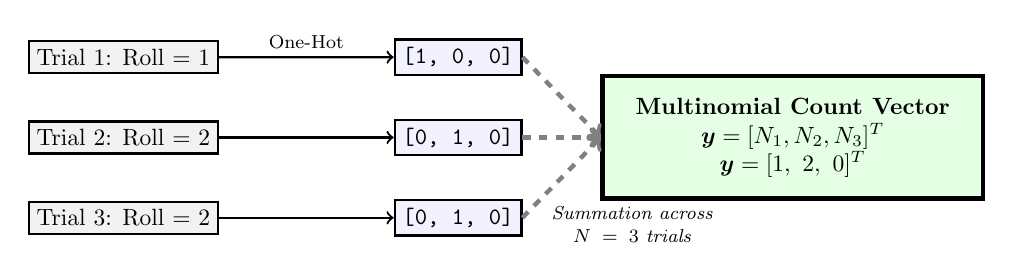
\begin{tikzpicture}[scale=0.85, every node/.style={transform shape}]
    % Structural Step 1: Raw categorical sequence
    \node[draw, thick, fill=gray!10, minimum width=2.5cm] (s1) at (0,3) {Trial 1: Roll = $1$};
    \node[draw, thick, fill=gray!10, minimum width=2.5cm] (s2) at (0,1.8) {Trial 2: Roll = $2$};
    \node[draw, thick, fill=gray!10, minimum width=2.5cm] (s3) at (0,0.6) {Trial 3: Roll = $2$};
    
    % Structural Step 2: One-hot maps
    \node[draw, thick, fill=blue!5, font=\ttfamily] (v1) at (5,3) {[1, 0, 0]};
    \node[draw, thick, fill=blue!5, font=\ttfamily] (v2) at (5,1.8) {[0, 1, 0]};
    \node[draw, thick, fill=blue!5, font=\ttfamily] (v3) at (5,0.6) {[0, 1, 0]};
    
    % Structural Step 3: Multinomial Aggregation
    \node[draw, ultra thick, fill=green!10, inner sep=8pt] (agg) at (10,1.8) {
        \begin{tabular}{c}
            \textbf{Multinomial Count Vector} \\
            $\bm{y} = [N_1, N_2, N_3]^T$ \\
            $\bm{y} = [1, \,\, 2, \,\, 0]^T$
        \end{tabular}
    };
    
    % Directional Arrows
    \draw[->, thick] (s1) -- (v1) node[midway, above] {\footnotesize One-Hot};
    \draw[->, thick] (s2) -- (v2);
    \draw[->, thick] (s3) -- (v3);
    
    \draw[->, ultra thick, dashed, gray] (v1.east) -- (agg.west);
    \draw[->, ultra thick, dashed, gray] (v2.east) -- (agg.west);
    \draw[->, ultra thick, dashed, gray] (v3.east) -- (agg.west);
    
    \node[text width=3cm, align=center, font=\footnotesize\itshape] at (7.6, 0.5) {Summation across \\ $N=3$ trials};
\end{tikzpicture}
\end{center}

\subsubsection*{6. Deep-Dive: Intuition Behind Vector Encoding Mechanisms}

To understand why the categorical probability mass function (PMF) is framed using algebraic products and exponents rather than traditional conditional logic statements, consider a concrete machine learning classification problem.

Suppose a model is trained to classify an image into one of $C=3$ distinct, qualitative categories: $\text{Class 1: Cat}$, $\text{Class 2: Dog}$, and $\text{Class 3: Bird}$. For a given input image, the model outputs a predicted probability parameter vector:
\begin{equation}
    \boldsymbol{\theta} = [\theta_1, \, \theta_2, \, \theta_3]^T = [0.20, \, 0.50, \, 0.30]^T
\end{equation}
Assume the ground-truth observation for this specific image is a \textbf{Dog}. We want our mathematical formulation to dynamically parse this distribution and cleanly isolate the target probability ($\theta_2 = 0.50$).

\paragraph{6.1. The Indicator Function Mechanical Breakdown}
In the indicator formulation, the ground-truth label is represented as a scalar index coordinate: $y = 2$. The categorical PMF expands across all $C$ available classes as a unified multiplication chain:
\begin{equation}
    \text{Cat}(y=2 \mid \boldsymbol{\theta}) = \prod_{c=1}^{3} \theta_c^{I(y = c)} = \theta_1^{I(2=1)} \times \theta_2^{I(2=2)} \times \theta_3^{I(2=3)}
\end{equation}
The evaluation path is governed entirely by the indicator exponent $I(y=c)$, which acts as an algebraic true/false matching switch:
\begin{itemize}
    \item \textbf{For $c=1$ (Cat):} The condition $y=1$ is false $\implies I(2=1) = 0 \implies \theta_1^0 = 0.20^0 = \mathbf{1}$
    \item \textbf{For $c=2$ (Dog):} The condition $y=2$ is true $\implies I(2=2) = 1 \implies \theta_2^1 = 0.50^1 = \mathbf{0.50}$
    \item \textbf{For $c=3$ (Bird):} The condition $y=3$ is false $\implies I(2=3) = 0 \implies \theta_3^0 = 0.30^0 = \mathbf{1}$
\end{itemize}
Multiplying these evaluations together demonstrates how the irrelevant classes mathematically dissolve out of the equation:
\begin{equation}
    \text{Cat}(y=2 \mid \boldsymbol{\theta}) = 1 \times 0.50 \times 1 = \mathbf{0.50}
\end{equation}

\paragraph{6.2. The One-Hot Vector Mechanical Breakdown}
In the one-hot encoding formulation, the true scalar label is mapped to a sparse binary vector: $\boldsymbol{y} = [0, \, 1, \, 0]^T$, where $y_1=0$, $y_2=1$, and $y_3=0$. The PMF evaluates using this configuration directly:
\begin{equation}
    \text{Cat}(\boldsymbol{y} \mid \boldsymbol{\theta}) = \prod_{c=1}^{3} \theta_c^{y_c} = \theta_1^{y_1} \times \theta_2^{y_2} \times \theta_3^{y_3}
\end{equation}
Instead of computing a matching logical test during runtime execution, the pre-built binary attributes inside the vector $\boldsymbol{y}$ serve directly as the powers:
\begin{equation}
    \text{Cat}(\boldsymbol{y} \mid \boldsymbol{\theta}) = 0.20^0 \times 0.50^1 \times 0.30^0 = 1 \times 0.50 \times 1 = \mathbf{0.50}
\end{equation}

\begin{tcolorbox}[colback=blue!5!white, colframe=blue!60!black, title=Why Avoid Conditional Code Branching?]
While standard desktop software handles class matching via an \texttt{if/else} statement, modern deep learning architectures evaluate gradients across millions of data observations concurrently. Logical branching splits execution pathways, causing execution stalls on vectorized hardware configurations (GPUs and TPUs). Converting selection logic into an algebraic product of exponents allows highly parallelized matrix math computations at maximum hardware speed.
\end{tcolorbox}

\section*{The Softmax Function and Log-Sum-Exp Trick}

To extend the categorical framework to supervised learning tasks where outcomes depend on an input vector $\boldsymbol{x}$, we transition from static parameters to conditional parameterization models.

\subsubsection*{1. Conditional Categorical Distributions and Logits}
In conditional multi-class classification, we define the probability of observing label $y$ given a feature vector $\boldsymbol{x}$ and model parameters $\boldsymbol{\theta}$ as a conditional categorical distribution:
\begin{equation}
    p(y \mid \boldsymbol{x}, \boldsymbol{\theta}) = \text{Cat}(y \mid \boldsymbol{f}(\boldsymbol{x}; \boldsymbol{\theta})) = \mathcal{M}(y \mid 1, \boldsymbol{f}(\boldsymbol{x}; \boldsymbol{\theta}))
\end{equation}
The underlying function $\boldsymbol{f}: \mathbb{R}^D \to \mathbb{R}^C$ maps the feature space to a valid $C$-dimensional probability vector. This requires satisfying the standard validation boundaries:
\begin{equation}
    0 \le f_c(\boldsymbol{x}; \boldsymbol{\theta}) \le 1 \quad \forall c \in \{1,\dots,C\} \quad \text{and} \quad \sum_{c=1}^{C} f_c(\boldsymbol{x}; \boldsymbol{\theta}) = 1
\end{equation}
Directly forcing a neural network or linear model to output bounded, sum-to-one values is mathematically cumbersome. To bypass this restriction, models instead compute unconstrained raw scores $\boldsymbol{a} = \boldsymbol{f}(\boldsymbol{x}; \boldsymbol{\theta}) \in \mathbb{R}^C$, known as \textbf{logits} (a multi-class generalization of log-odds). These logits are then projected into a valid probability simplex via the \textbf{softmax function}:
\begin{equation}
    \text{softmax}(\boldsymbol{a}) \triangleq \left[ \frac{e^{a_1}}{\sum_{c'=1}^{C} e^{a_{c'}}}, \, \frac{e^{a_2}}{\sum_{c'=1}^{C} e^{a_{c'}}}, \, \dots, \, \frac{e^{a_C}}{\sum_{c'=1}^{C} e^{a_{c'}}} \right]^T
\end{equation}

\subsubsection*{2. The Effect of Temperature Scaling}
The softmax function earns its name because it operates as a smooth, differentiable approximation of the maximum selector function ($\text{argmax}$). We can manipulate the sharpness of this distribution by introducing a positive scalar constant $T > 0$, known as the \textbf{temperature}:
\begin{equation}
    \text{softmax}\left(\frac{\boldsymbol{a}}{T}\right)_c = \frac{e^{a_c / T}}{\sum_{c'=1}^{C} e^{a_{c'} / T}}
\end{equation}
Modulating this parameter alters the structural entropy of the output space:
\begin{itemize}
    \item \textbf{Low Temperature ($T \to 0$):} The distribution sharpens into a rigid "winner-takes-all" landscape, shifting all probability mass toward the single most probable state:
    \begin{equation}
        \lim_{T \to 0} \text{softmax}\left(\frac{\boldsymbol{a}}{T}\right)_c = 
        \begin{cases} 
            1.0 & \text{if } c = \text{argmax}_{c'} \, a_{c'} \\ 
            0.0 & \text{otherwise} 
        \end{cases}
    \end{equation}
    \item \textbf{High Temperature ($T \to \infty$):} The relative differences between logits are compressed, forcing the probability mass to spread uniformly across all $C$ options:
    \begin{equation}
        \lim_{T \to \infty} \text{softmax}\left(\frac{\boldsymbol{a}}{T}\right)_c = \frac{1}{C}
    \end{equation}
\end{itemize}

\subsubsection*{3. Numerical Instability and the Log-Sum-Exp Trick}
When executing softmax predictions on digital computers, evaluating raw exponentials exposes calculations to severe numerical risks when dealing with the partition function $Z(\boldsymbol{a}) = \sum_{c'=1}^C e^{a_{c'}}$:
\begin{itemize}
    \item \textbf{Overflow:} If $\boldsymbol{a} = [1000, \, 1001, \, 1000]^T$, calculating $e^{1001}$ results in computer memory reading standard 64-bit precision limits as infinity (\texttt{inf}), rendering the normalization division operations invalid.
    \item \textbf{Underflow:} If $\boldsymbol{a} = [-1000, \, -999, \, -1000]^T$, the individual terms collapse prematurely to zero ($e^{-1000} \to 0$), producing a fatal division-by-zero error ($Z = 0$).
\end{itemize}
To eliminate these precision failures, we inject an arbitrary shift constant $m$ utilizing the algebraic \textbf{log-sum-exp identity}:
\begin{equation}
    \log \sum_{c=1}^{C} \exp(a_c) = m + \log \sum_{c=1}^{C} \exp(a_c - m)
\end{equation}
By setting $m = \max_c a_c$, the largest exponent inside the evaluation array is forced to exactly $a_c - m = 0$, guaranteeing that $e^0 = 1$. This blocks structural overflow limits completely, while preserving underflow limits within reasonable bounds. We encapsulate this operation inside the $\text{lse}(\boldsymbol{a})$ function definition:
\begin{equation}
    \text{lse}(\boldsymbol{a}) \triangleq \log \sum_{c=1}^{C} \exp(a_c)
\end{equation}
Using this definition, normalized conditional probabilities are computed stably in log-space before applying the final outer exponential scaling:
\begin{equation}
    p(y = c \mid \boldsymbol{x}) = \exp\big(a_c - \text{lse}(\boldsymbol{a})\big)
\end{equation}

\begin{tcolorbox}[colback=red!5!white, colframe=red!60!black, title=Numerical Verification Example]
Let us resolve our unstable overflow example vector $\boldsymbol{a} = [1000, \, 1001, \, 1000]^T$. \\
Set the stabilizing shift factor: $m = \max(1000, 1001, 1000) = 1001$. \\
Subtract $m$ from each element to create shifted logits: $\boldsymbol{a} - m = [-1, \, 0, \, -1]^T$. 

Now, compute the stable partition vector under the LSE identity:
\begin{align*}
    \text{lse}(\boldsymbol{a}) &= 1001 + \log\left(e^{-1} + e^0 + e^{-1}\right) \\
    &= 1001 + \log\left(0.3679 + 1.0000 + 0.3679\right) \\
    &= 1001 + \log(1.7358) = 1001 + 0.5515 = \mathbf{1001.5515}
\end{align*}
Finally, calculate the exact, overflow-free probability value for Class 2:
\begin{equation*}
    p(y=2 \mid \boldsymbol{x}) = \exp\big(1001 - 1001.5515\big) = \exp(-0.5515) = \mathbf{0.576}
\end{equation*}
\end{tcolorbox}

\subsubsection*{4. Optimization and Stable Cross-Entropy Loss Integration}
To maximize pipeline efficiency during optimization routines, machine learning backends fuse the softmax layer and cross-entropy loss function into a single computational block that acts directly on logits $\boldsymbol{a}$ instead of probability vectors $\boldsymbol{p}$. 

Consider the binary classification sequence loss landscape ($C=2$):
\begin{equation}
    \mathcal{L} = - \big[\mathbb{I}(y = 0) \log p_0 + \mathbb{I}(y = 1) \log p_1\big]
\end{equation}
Instead of calculating intermediate probabilities, we express the isolated scalar loss computations using integrated $\text{lse}$ shifts:
\begin{equation}
    \log p_1 = \log \left( \frac{1}{1 + \exp(-a)} \right) = \log(1) - \log\big(1 + \exp(-a)\big) = 0 - \text{lse}([0, \, -a]^T)
\end{equation}
\begin{equation}
    \log p_0 = 0 - \text{lse}([0, \, +a]^T)
\end{equation}
This formulation preserves clean gradients and numerical precision throughout backward propagation sequences, even when individual logits reach extreme values.

\subsubsection*{5. Concrete Numerical Example: Stable Binary Cross-Entropy Fusing}

To see exactly how this fused formulation saves a computer from a memory meltdown, let us trace a binary classification scenario ($C=2$) with an extreme logit value.

Suppose an image classification model is evaluated on a true baseline label of \textbf{Class 0} ($y=0$). However, the model is aggressively confident in the wrong answer, spitting out an extreme single relative logit score of:
\begin{equation}
    a = 1000
\end{equation}

\paragraph{The Naive Calculation Failure:}
If the execution backend processes this calculation sequentially, it must first compute the standalone probability for the true class $p_0$ using the standard sigmoid function:
\begin{equation}
    p_0 = \frac{1}{1 + \exp(a)} = \frac{1}{1 + \exp(1000)}
\end{equation}
Because $\exp(1000)$ evaluates directly to \texttt{inf} (infinity) in 64-bit computer precision, the denominator overflows, forcing the probability down to absolute zero ($p_0 = \frac{1}{\infty} \to 0.0$). 

Next, the separate cross-entropy loss block attempts to evaluate the penalty for this training instance:
\begin{equation}
    \mathcal{L} = -\log p_0 = -\log(0.0) = -(-\infty) = \mathbf{\infty} \quad \longrightarrow \quad \text{\textbf{FATAL ERROR (NaN)}}
\end{equation}
The loss becomes infinity, which physically breaks the optimization pipeline because backpropagation cannot calculate a valid derivative (gradient) from an infinite value.

\paragraph{The Fused Log-Sum-Exp Solution:}
Now let us watch how the integrated backend evaluates the exact same scenario using Equation (123) to solve for $\log p_0$ directly from the logit $a = 1000$, without ever calculating $p_0$ as an intermediate step:
\begin{equation}
    \log p_0 = 0 - \text{lse}([0, \, +a]^T) = 0 - \text{lse}([0, \, 1000]^T)
\end{equation}

\noindent \textbf{Step 1: Identify and apply the max shift parameter ($m$)}
Find the maximum value inside the target array $[0, 1000]^T$:
\begin{equation}
    m = \max(0, 1000) = 1000
\end{equation}
Subtract $m$ from both terms inside the log-space vector to stabilize the exponents:
\begin{equation}
    \text{lse}([0, \, 1000]^T) = 1000 + \log\left(\exp(0 - 1000) + \exp(1000 - 1000)\right)
\end{equation}

\noindent \textbf{Step 2: Evaluate the shifted exponential elements}
\begin{align*}
    \text{lse}([0, \, 1000]^T) &= 1000 + \log\left(\exp(-1000) + \exp(0)\right) \\
    &= 1000 + \log(0.0 + 1.0) \\
    &= 1000 + \log(1.0) \\
    &= 1000 + 0 = \mathbf{1000}
\end{align*}
Notice that $\exp(-1000)$ safely underflows to $0.0$, which is completely harmless to the addition block. 

\noindent \textbf{Step 3: Compute final stable loss values}
We plug this clean scalar value back into our fused loss formula:
\begin{equation}
    \log p_0 = 0 - 1000 = -1000
\end{equation}
\begin{equation}
    \mathcal{L} = -\log p_0 = -(-1000) = \mathbf{1000.0}
\end{equation}

\begin{tcolorbox}[colback=blue!5!white, colframe=blue!60!black, title=Core Takeaway]
By fusing the operations, the cross-entropy loss scales perfectly and linearly as $\mathcal{L} = 1000.0$. The computer completely sidesteps the intermediate $\log(0)$ trap. The gradient remains perfectly stable, allowing the optimization engine to compute clean weight updates and smoothly correct the model's error.
\end{tcolorbox}

\section*{The Univariate Gaussian (Normal) Distribution}

The most widely used continuous probability distribution for modeling real-valued scalar random variables $y \in \mathbb{R}$ is the \textbf{Gaussian distribution}, also famously known as the \textbf{normal distribution}. It provides the bedrock for modeling measurement errors, noise profiles, and physical phenomena across machine learning architectures due to its mathematical tractability and its emergence from the Central Limit Theorem.

\subsubsection*{1. The Cumulative Distribution Function (CDF)}
To understand any continuous random variable $Y$, we begin with its foundational cumulative metric. We define the \textbf{cumulative distribution function (CDF)}, denoted by an uppercase letter $P$, as:
\begin{equation}
    P(y) \triangleq \Pr(Y \le y)
\end{equation}
By tracking cumulative totals, the CDF maps a real value $y$ to a probability scale $[0, 1]$. Because probabilities cannot decrease as we accumulate more area along the real number line, all CDFs are mathematically guaranteed to be \textbf{monotonically non-decreasing functions}. If we wish to calculate the exact probability of a variable falling within a localized spatial interval $(a, b]$, we evaluate the difference between its boundary endpoints:
\begin{equation}
    \Pr(a < Y \le b) = P(b) - P(a)
\end{equation}

For a Gaussian random variable, we denote its specific parameterized CDF using the Greek symbol $\Phi$. It represents the cumulative area under the bell curve starting from negative infinity up to a target threshold score $y$:
\begin{equation}
    \Phi(y; \mu, \sigma^2) \triangleq \int_{-\infty}^{y} \mathcal{N}(z \mid \mu, \sigma^2) \, dz
\end{equation}
Where the parameter $\mu$ encodes the **mean** (and the central peak/mode) of the distribution, and $\sigma^2$ encodes the **variance** (the spread). Alternatively, we sometimes quantify a Gaussian's dispersion using the \textbf{precision} parameter, defined as the inverse variance ($\lambda = \frac{1}{\sigma^2}$). When a Gaussian distribution has a mean of zero and a variance of one ($\mu = 0, \sigma = 1$), it is uniquely termed the \textbf{standard normal distribution}.

Because this integral has no closed-form analytical solution, software applications compute the Gaussian CDF using numerical approximations derived from the \textbf{error function} ($\text{erf}$):
\begin{equation}
    \Phi(y; \mu, \sigma^2) = \frac{1}{2} \left[ 1 + \text{erf}\left( \frac{y - \mu}{\sigma\sqrt{2}} \right) \right]
\end{equation}
where the error function $\text{erf}(u)$ acts as a foundational mathematical tool defined as:
\begin{equation}
    \text{erf}(u) \triangleq \frac{2}{\sqrt{\pi}} \int_{0}^{u} e^{-t^2} \, dt
\end{equation}

\paragraph{Quantiles and the Probit Function:}
The inverse of the CDF, denoted $P^{-1}(q)$, allows us to reverse our perspective. Given a target probability mass $q \in [0, 1]$, the inverse function returns the corresponding spatial value $y_q$ such that $\Pr(Y \le y_q) = q$. This value is termed the **$q$-th quantile**.
\begin{itemize}
    \item \textbf{The Median:} The $0.50$ quantile ($P^{-1}(0.5)$) is the literal median of the distribution, splitting the probability mass cleanly in half. Due to the perfect reflectional symmetry of the Gaussian bell curve, its mean, mode, and median are identical ($\text{median} = \mu$).
    \item \textbf{Quartiles:} The values $P^{-1}(0.25)$ and $P^{-1}(0.75)$ mark the lower and upper quartiles, segmenting the core data pool into quarters.
\end{itemize}

The inverse CDF of a standard normal distribution $\Phi^{-1}$ is known as the \textbf{probit function}. By leveraging the symmetric profile of the standard normal distribution, we can construct bounded confidence zones. For instance, points to the left of the quantile $\Phi^{-1}(\alpha/2)$ isolate exactly $\alpha/2$ of the total probability mass. Symmetrically, points to the right of $\Phi^{-1}(1 - \alpha/2)$ contain an identical $\alpha/2$ mass. Therefore, the central interval bounded by these two coordinates contains exactly $1 - \alpha$ of the total distribution mass:
\begin{equation}
    \text{Central Interval} = \left( \Phi^{-1}\left(\frac{\alpha}{2}\right), \, \Phi^{-1}\left(1 - \frac{\alpha}{2}\right) \right)
\end{equation}

If we target a standard $95\%$ certainty window ($\alpha = 0.05$), our tail limits are evaluated as:
\begin{equation}
    \left( \Phi^{-1}(0.025), \, \Phi^{-1}(0.975) \right) = (-1.96, \, 1.96)
\end{equation}
For a general Gaussian model scaled to a custom parameter configuration $\mathcal{N}(\mu, \sigma^2)$, this bounds our $95\%$ mass within the range $(\mu - 1.96\sigma, \, \mu + 1.96\sigma)$, which engineers frequently approximate using the foundational **$\mu \pm 2\sigma$ empirical rule**.

\begin{tcolorbox}[colback=blue!5!white, colframe=blue!60!black, title=Geometric Intuition: The 95\% Interval]
The value $1.96$ is not an arbitrary constant; it indicates that traveling approximately two standard deviations away from the center of a normal distribution in both directions forms a geometric window that traps exactly $95\%$ of all physical samples generated by that system. The remaining $5\%$ is split into two equal $2.5\%$ tails on the extreme left and right margins.
\end{tcolorbox}

\subsubsection*{2. The Probability Density Function (PDF)}
While the CDF tells us the probability of landing *below* a certain value, the \textbf{probability density function (PDF)}, written with a lowercase $p(y)$, tells us the relative likelihood of landing at a specific coordinate. It is defined mathematically as the derivative of the continuous CDF:
\begin{equation}
    p(y) \triangleq \frac{d}{dy} P(y)
\end{equation}
Evaluating this derivative for a Gaussian variable yields the iconic bell-shaped density function:
\begin{equation}
    \mathcal{N}(y \mid \mu, \sigma^2) \triangleq \frac{1}{\sqrt{2\pi\sigma^2}} \exp\left( -\frac{1}{2\sigma^2}(y - \mu)^2 \right) = \phi(y; \mu, \sigma^2)
\end{equation}
where the term $\frac{1}{\sqrt{2\pi\sigma^2}}$ serves as the mandatory \textbf{normalization constant}. This constant ensures that the total area trapped under the curve integrates to exactly $1.0$, satisfying the foundational law of total probability. When dealing with a standard normal distribution ($\mu=0, \sigma=1$), this density profile collapses to a simplified baseline denoted by $\phi(y)$.

Given a continuous density function, we extract real probability masses by integrating over a defined interval:
\begin{equation}
    \Pr(a < Y \le b) = \int_{a}^{b} p(y) \, dy = P(b) - P(a)
\end{equation}
If we narrow our focus down to a vanishingly small spatial element of width $dy$, the probability can be accurately approximated as a simple rectangle:
\begin{equation}
    \Pr(y \le Y \le y + dy) \approx p(y) \, dy
\end{equation}
This tells us that the absolute probability of hitting a small window is the **density height at that point times the spatial width of the window**.

\begin{tcolorbox}[colback=red!5!white, colframe=red!60!black, title=Critical Concept: Density is NOT Probability]
A common mistake is assuming that a probability density cannot exceed $1.0$. Remember, $p(y)$ is a *relative height*, not a percentage. If a distribution is heavily squeezed by a small variance, the curve must shoot upward to ensure the total area underneath stays equal to $1.0$. 

For example, calculating the peak density of a narrow Gaussian with $\mu=0$ and $\sigma^2=0.1$:
\begin{equation*}
    \mathcal{N}(0 \mid 0, \, 0.1) = \frac{1}{\sqrt{2\pi(0.1)}} \exp(0) = \frac{1}{\sqrt{0.6283}} \times 1 \approx \mathbf{3.99}
\end{equation*}
A density value of $3.99$ is completely valid because when you multiply it by a tiny spatial width $dy$, the resulting probability product will always remain $\le 1.0$.
\end{tcolorbox}

\subsubsection*{3. Statistical Moments: Mathematical Derivations}
We leverage the PDF to calculate the definitive shape properties (moments) of a continuous distribution.

\paragraph{First Raw Moment - Expected Value (Mean):}
The expected value $\mathbb{E}[Y]$ represents the long-run average center of mass of the continuous random variable:
\begin{equation}
    \mathbb{E}[Y] \triangleq \int_{-\infty}^{\infty} y \, p(y) \, dy
\end{equation}
Evaluating this integral for a Gaussian distribution yields its location parameter directly:
\begin{equation}
    \mathbb{E}\big[\mathcal{N}(\cdot \mid \mu, \sigma^2)\big] = \mu
\end{equation}

\paragraph{Second Central Moment - Variance:}
The variance $\mathbb{V}[Y]$ measures the descriptive "spread" or dispersion of the distribution around its mean center. It computes the average squared deviation:
\begin{equation}
    \mathbb{V}[Y] \triangleq \mathbb{E}\left[ (Y - \mu)^2 \right] = \int_{-\infty}^{\infty} (y - \mu)^2 \, p(y) \, dy
\end{equation}
We can derive a highly useful alternative identity for variance by expanding the algebraic squared term inside the integration operator:
\begin{align}
    \mathbb{V}[Y] &= \int_{-\infty}^{\infty} (y^2 - 2\mu y + \mu^2) \, p(y) \, dy \\
    &= \int_{-\infty}^{\infty} y^2 p(y) \, dy + \mu^2 \int_{-\infty}^{\infty} p(y) \, dy - 2\mu \int_{-\infty}^{\infty} y p(y) \, dy
\end{align}
By applying basic axioms of probability, we know that:
\begin{itemize}
    \item $\int_{-\infty}^{\infty} p(y) \, dy = 1$ \quad (The total probability density must integrate to 1)
    \item $\int_{-\infty}^{\infty} y p(y) \, dy = \mu$ \quad (The definition of the expected value $\mathbb{E}[Y]$)
    \item $\int_{-\infty}^{\infty} y^2 p(y) \, dy = \mathbb{E}[Y^2]$ \quad (The second raw moment)
\end{itemize}
Substituting these terms back into our expanded equation yields the standard variance identity:
\begin{equation}
    \mathbb{V}[Y] = \mathbb{E}[Y^2] + \mu^2(1) - 2\mu(\mu) = \mathbb{E}[Y^2] - \mu^2
\end{equation}
Rearranging this relationship reveals a valuable formula for calculating the second raw moment:
\begin{equation}
    \mathbb{E}[Y^2] = \sigma^2 + \mu^2
\end{equation}

\paragraph{Standard Deviation:}
Because variance is measured in squared units (e.g., if $Y$ is in meters, variance is in $\text{meters}^2$), it can be difficult to interpret intuitively. To align our dispersion metrics with the original units of the random variable, we define the \textbf{standard deviation} as the positive square root of the variance:
\begin{equation}
    \text{std}[Y] \triangleq \sqrt{\mathbb{V}[Y]} = \sigma
\end{equation}
For a Gaussian distribution, evaluating this metric returns its precise scale parameter: $\text{std}\big[\mathcal{N}(\cdot \mid \mu, \sigma^2)\big] = \sigma$.

\subsubsection*{4. Gaussian Regression (Conditional Modeling)}
So far, we have analyzed the \textit{unconditional} Gaussian distribution, where the mean $\mu$ and variance $\sigma^2$ are static parameters optimized across an entire dataset. In supervised machine learning, however, we want our predictions to dynamically react to an input vector $\mathbf{x} \in \mathbb{R}^D$. To achieve this, we transition to a \textbf{conditional density model}:
\begin{equation}
    p(y \mid \mathbf{x}; \boldsymbol{\theta}) = \mathcal{N}\left(y \mid f_\mu(\mathbf{x}; \boldsymbol{\theta}), \, f_\sigma(\mathbf{x}; \boldsymbol{\theta})^2\right)
\end{equation}
Here, the distribution parameters are no longer constants; they are driven by two distinct function mappings:
\begin{itemize}
    \item $f_\mu(\mathbf{x}; \boldsymbol{\theta}) \in \mathbb{R}$: A regression model (e.g., a neural network or linear layer) that predicts the conditional mean center for input $\mathbf{x}$.
    \item $f_\sigma(\mathbf{x}; \boldsymbol{\theta})^2 \in \mathbb{R}^+$: A regression model that outputs a strictly positive value representing the conditional variance at input $\mathbf{x}$.
\end{itemize}

\subsubsection*{5. Homoscedastic vs. Heteroskedastic Formulations}

Depending on how we model the variance function $f_\sigma(\mathbf{x}; \boldsymbol{\theta})^2$, conditional Gaussian models split into two foundational paradigms:

\paragraph{1. Homoscedastic Regression (Constant Noise)}
The most common baseline assumption is that the data noise is completely uniform across the entire input space, meaning variance is independent of $\mathbf{x}$. If we pair this with a linear function for our mean, we get standard **Linear Regression**:
\begin{equation}
    p(y \mid \mathbf{x}; \boldsymbol{\theta}) = \mathcal{N}\left(y \mid \mathbf{w}^T\mathbf{x} + b, \, \sigma^2\right)
\end{equation}
where the shared parameter vector is explicitly bundled as $\boldsymbol{\theta} = (\mathbf{w}, b, \sigma^2)$. In this setting, changing $\mathbf{x}$ shifts the center location of the bell curve along the prediction line, but the overall width and shape of the distribution remain completely frozen.

\paragraph{2. Heteroskedastic Regression (Input-Dependent Noise)}
In many real-world scenarios (such as financial forecasting or physical systems), the level of data noise changes drastically depending on where you look in the input space. Letting our variance model adapt dynamically to the input yields **Heteroskedastic Regression**:
\begin{equation}
    p(y \mid \mathbf{x}; \boldsymbol{\theta}) = \mathcal{N}\left(y \mid \mathbf{w}_\mu^T\mathbf{x} + b, \, \sigma_+^2(\mathbf{w}_\sigma^T\mathbf{x})\right)
\end{equation}
Here, we optimize two separate sets of parameters: $\mathbf{w}_\mu$ to track the structural trend, and $\mathbf{w}_\sigma$ to track data volatility. Because unconstrained linear layers can easily output negative numbers—which would break our variance calculation—we pass the variance logit through the \textbf{softplus function}:
\begin{equation}
    \sigma_+(a) \triangleq \log(1 + e^a)
\end{equation}
The softplus function acts as a smooth, differentiable approximation of the ReLU activation function, cleanly mapping any real value $a \in \mathbb{R}$ to a strictly positive domain $\mathbb{R}^+$, ensuring our predicted standard deviation never falls below zero.

\begin{tcolorbox}[colback=blue!5!white, colframe=blue!60!black, title=Intuitive Visualization: Homoscedastic vs. Heteroskedastic]
\begin{itemize}
    \item \textbf{Homoscedasticity:} Imagine a scatter plot of data points wrapped cleanly inside a uniform tube of constant thickness running along a regression line. The model's uncertainty about any single point is identical everywhere.
    \item \textbf{Heteroskedasticity:} Imagine a megaphone shape. For small values of $\mathbf{x}$, the data points tightly hug the regression line (low variance). As $\mathbf{x}$ grows, the points spray widely outward in a broad cloud (high variance). The model learns to be confident in some regions and highly cautious in others.
\end{itemize}
\end{tcolorbox}

\subsubsection*{6. Deconstructing Predictive Uncertainty vs. Parameter Uncertainty}
When evaluating a model's prediction errors, it is vital to distinguish between two completely different types of statistical uncertainty:

\paragraph{Aleatoric (Predictive) Uncertainty:}
This represents the natural, irreducible noise inherent in the data-generating process itself. Geometrically, if we plot the $95\%$ predictive interval around our conditional mean:
\begin{equation}
    \text{95\% Interval} = \big[\mu(\mathbf{x}) - 1.96\sigma(\mathbf{x}), \,\, \mu(\mathbf{x}) + 1.96\sigma(\mathbf{x})\big] \approx \mu(\mathbf{x}) \pm 2\sigma(\mathbf{x})
\end{equation}
this window measures our uncertainty regarding the next raw observation $y$. It accounts for the random fluctuations of the physical system and cannot be eliminated by collecting more training data.

\paragraph{Epistemic (Parameter) Uncertainty:}
This measures the uncertainty in our model's underlying parameter estimates $\boldsymbol{\theta}$, representing our doubt about whether we have discovered the true, noise-free regression line. It is quantified as the square root of the parameter variance:
\begin{equation}
    \text{Parameter Uncertainty} = \sqrt{\mathbb{V}\big[f_\mu(\mathbf{x}; \boldsymbol{\theta})\big]}
\end{equation}
Notice that this calculation does not contain the data noise term $\sigma$. Epistemic uncertainty stems purely from a lack of information; it can be driven down toward zero by feeding more data points into the optimization pipeline to solidify our parameter estimates.

\subsubsection*{7. Foundational Pillars of the Gaussian Ubiquity}
The Gaussian distribution is the undisputed default choice in statistics and machine learning. This widespread ubiquity rests on four core pillars:

\begin{enumerate}
    \item \textbf{Interpretability:} It is completely defined by two simple parameters that match our natural descriptive statistics: the mean $\mu$ (center of mass) and the variance $\sigma^2$ (geometric spread).
    \item \textbf{The Central Limit Theorem (CLT):} The CLT guarantees that when you sum a large number of independent, identically distributed random variables, their collective distribution naturally converges to a standard Gaussian shape—regardless of the original distribution of the individual variables. This makes it a highly accurate choice for modeling composite residual noise.
    \item \textbf{The Maximum Entropy Principle:} If you are tasked with choosing a continuous probability distribution with a specific mean and variance, but you want to avoid making any other arbitrary assumptions about its shape, the Gaussian distribution is mathematically proven to be the uniquely correct choice. It maximizes informational entropy, ensuring it is the least biased default model possible.
    \item \textbf{Analytical Tractability:} Its quadratic exponential form yields clean, elegant derivatives. This allows developers to design highly parallelized, closed-form algorithmic solutions that are exceptionally cheap to execute on modern hardware architectures.
\end{enumerate}

\begin{tcolorbox}[colback=red!5!white, colframe=red!60!black, title=Historical Clarification: What's in a Name?]
Calling this distribution "Gaussian" is technically an anachronism. The fundamental nature and properties of the normal distribution were detailed by Pierre-Simon Laplace when Carl Friedrich Gauss was only six years old, and Abraham de Moivre had documented its core behavior before Laplace was even born. However, Gauss popularized its practical applications for tracking astronomical orbits in the 1800s. 

Similarly, the term "normal distribution" should be used with caution. It originated from the "normal equations" used in linear least-squares regression. Using the word "normal" can accidentally imply that other distributions are "abnormal," when in reality, the Gaussian distribution is the true mathematical anomaly due to its unique convergence properties.
\end{tcolorbox}

\subsubsection*{8. The Dirac Delta Function as a Limiting Case}
As the variance of a continuous Gaussian distribution collapses toward zero ($\sigma \to 0$), the geometric profile of the bell curve undergoes an extreme transformation. The distribution narrows down into an infinitely sharp, infinitely tall "spike" anchored precisely at the mean $\mu$. 

We express this limiting behavior mathematically as:
\begin{equation}
    \lim_{\sigma \to 0} \mathcal{N}(y \mid \mu, \, \sigma^2) \longrightarrow \delta(y - \mu) \tag{2.124}
\end{equation}
where $\delta$ is the \textbf{Dirac delta function}, defined by the piecewise behavior:
\begin{equation}
    \delta(x) = \begin{cases} 
        +\infty & \text{if } x = 0 \\ 
        0 & \text{if } x \neq 0 
    \end{cases} \tag{2.125}
\end{equation}
Despite its infinite height at the origin, the Dirac delta function is constrained by a fundamental property: its total integrated mass over all real space must equal exactly $1.0$:
\begin{equation}
    \int_{-\infty}^{\infty} \delta(x) \, dx = 1 \tag{2.126}
\end{equation}

A slight notation variant defines the delta function centered explicitly around a specific point $y$:
\begin{equation}
    \delta_y(x) = \begin{cases} 
        +\infty & \text{if } x = y \\ 
        0 & \text{if } x \neq y 
    \end{cases} \tag{2.127}
\end{equation}
This allows us to write the coordinate shift interchangeably as:
\begin{equation}
    \delta_y(x) = \delta(x - y) \tag{2.128}
\end{equation}

\paragraph{The Sifting Property:}
Because the Dirac delta function evaluates to zero everywhere except at the exact point where its argument is zero, multiplying it by any continuous function $f(y)$ and integrating isolates ("sifts") the value of that function at that specific localized point:
\begin{equation}
    \int_{-\infty}^{\infty} f(y) \delta(x - y) \, dy = f(x) \tag{2.129}
\end{equation}

\begin{tcolorbox}[colback=blue!5!white, colframe=blue!60!black, title=Numerical Intuition: The Vanishing Variance Spike]
Let us calculate the peak height of a centered standard Gaussian ($\mu=0$) at $y=0$ as we systematically shrink the variance ($\sigma^2$) toward zero:
\begin{equation*}
    \mathcal{N}(0 \mid 0, \, \sigma^2) = \frac{1}{\sqrt{2\pi\sigma^2}} \exp(0) = \frac{1}{\sigma\sqrt{2\pi}}
\end{equation*}
\begin{itemize}
    \item \textbf{At $\sigma = 1.0$:} $\text{Peak Height} = \frac{1}{1\sqrt{2\pi}} \approx \mathbf{0.3989}$
    \item \textbf{At $\sigma = 0.1$:} $\text{Peak Height} = \frac{1}{0.1\sqrt{2\pi}} \approx \mathbf{3.989}$
    \item \textbf{At $\sigma = 0.01$:} $\text{Peak Height} = \frac{1}{0.01\sqrt{2\pi}} \approx \mathbf{39.89}$
    \item \textbf{At $\sigma = 0.001$:} $\text{Peak Height} = \frac{1}{0.001\sqrt{2\pi}} \approx \mathbf{398.94}$
\end{itemize}
As $\sigma \to 0$, the height spikes toward infinity while the lateral spread drops to zero. However, because it is still fundamentally a normalized Gaussian at every step of the limit, the area under the curve remains perfectly locked at $1.0$. This limiting case allows machine learning models to represent discrete labels or deterministic targets using continuous probability calculus.
\end{tcolorbox}

\subsubsection*{9. The Truncated Gaussian Distribution}
In many domain applications, physical constraints dictate that a random variable cannot exist outside a specific window (for example, distances, ages, or bounds like image pixel ranges). To model this, we restrict the support of a standard Gaussian distribution to a fixed interval $(a, b)$. 

To ensure the remaining probability mass still sums to $1.0$, we divide the standard density formula by the total cumulative mass trapped within the target truncation boundaries:
\begin{equation}
    \mathcal{N}(x \mid \mu, \, \sigma^2, \, a, \, b) = \frac{1}{\sigma} \frac{\phi\left( \frac{x - \mu}{\sigma} \right)}{\Phi\left( \frac{b - \mu}{\sigma} \right) - \Phi\left( \frac{a - \mu}{\sigma} \right)} \mathbb{I}(a < x < b)
\end{equation}
where:
\begin{itemize}
    \item $\phi(u)$ is the standard normal probability density function (PDF).
    \item $\Phi(u)$ is the standard normal cumulative distribution function (CDF).
    \item $\mathbb{I}(a < x < b)$ is an indicator function that acts as a hard boundary wall, returning $1$ if $x$ falls inside the interval $(a, b)$ and $0$ otherwise.
\end{itemize}

\begin{tcolorbox}[colback=red!5!white, colframe=red!60!black, title=Numerical Verification: Semi-Infinite Slicing]
Suppose we want to truncate a standard normal distribution ($\mu=0, \sigma=1$) to support \textbf{only positive real numbers} ($a=0$ and $b=+\infty$). Let us construct the new scaled density function step-by-step:

\noindent \textbf{Step 1: Compute the boundary CDF values}
\begin{itemize}
    \item Lower Bound: $\Phi\left(\frac{a - \mu}{\sigma}\right) = \Phi\left(\frac{0 - 0}{1}\right) = \Phi(0) = \mathbf{0.50}$ (Exactly half the mass lies below 0)
    \item Upper Bound: $\Phi\left(\frac{b - \mu}{\sigma}\right) = \Phi\left(\frac{\infty - 0}{1}\right) = \Phi(\infty) = \mathbf{1.00}$
\end{itemize}

\noindent \textbf{Step 2: Evaluate the normalization denominator}
\begin{equation*}
    \text{Mass Remaining} = \Phi(\infty) - \Phi(0) = 1.00 - 0.50 = \mathbf{0.50}
\end{equation*}

\noindent \textbf{Step 3: Calculate the final scaled density profile}
Plugging these values into the truncation formula yields:
\begin{equation*}
    \mathcal{N}(x \mid 0, \, 1, \, 0, \, +\infty) = \frac{1}{1} \frac{\phi(x)}{0.50} \mathbb{I}(0 < x < +\infty) = \mathbf{2\phi(x)} \quad \text{for } x > 0
\end{equation*}
Because we cleanly sliced away the negative half of the distribution, the density of the remaining positive half must be exactly doubled to ensure that the newly formed distribution integrates over its modified domain to $1.0$.
\end{tcolorbox}

\section*{Study Guide: Core Properties, Derivations, and Calculations of the Gaussian Distribution}

This guide serves as an intuitive yet mathematically rigorous module for understanding the Univariate Gaussian (Normal) Distribution. We bridge the gap between high-level conceptual properties and the foundational calculus that proves them.

---

\subsection*{Module 1: Intuitive Properties of the Bell Curve}
Before diving into proofs, let us establish the fundamental geometric behaviors of the probability density function $\mathcal{N}(y \mid \mu, \sigma^2)$.

\begin{enumerate}
    \item \textbf{Perfect Bilateral Symmetry:} The curve is perfectly symmetrical around its center axis $y = \mu$. If you slice the distribution at the mean, the left half is a mirror reflection of the right half.
    \item \textbf{The Central Confluence (Unimodality):} The mean (average), median (middle point), and mode (highest peak) are not merely close—they are mathematically locked at the exact same coordinate ($y = \mu$).
    \item \textbf{Asymptotic Tails:} As you travel infinitely far to the left ($y \to -\infty$) or right ($y \to +\infty$), the density drops precipitously toward zero but never technically touches the horizontal axis. No matter how extreme the value, its probability density remains strictly greater than zero ($\phi(y) > 0$).
    \item \textbf{Inflection Points at Exactly $\mu \pm \sigma$:} If you look closely at the slope of the bell curve, it starts steep and begins to flatten out exactly one standard deviation away from the center. These points of maximum steepness are the mathematical inflection points of the function.
\end{enumerate}

---

\subsection*{Module 2: Foundational Mathematical Derivations}
To truly master the normal distribution, we must prove its properties from its raw definition:
\begin{equation}
    p(y) = \frac{1}{\sqrt{2\pi\sigma^2}} \exp\left( -\frac{1}{2\sigma^2}(y - \mu)^2 \right)
\end{equation}

\subsubsection*{Proof 1: The Total Area Under the Curve Equals 1}
To verify this is a valid probability distribution, we must show that the total integral $I = \int_{-\infty}^{\infty} p(y) \, dy = 1$. Let us isolate the hard part of the integral by performing a variable substitution. Let $u = \frac{y - \mu}{\sigma}$, which implies $dy = \sigma \, du$:
\begin{equation}
    I = \int_{-\infty}^{\infty} \frac{1}{\sqrt{2\pi\sigma^2}} e^{-\frac{1}{2}u^2} (\sigma \, du) = \frac{1}{\sqrt{2\pi}} \int_{-\infty}^{\infty} e^{-\frac{1}{2}u^2} \, du
\end{equation}
Let us define the core integral as $J = \int_{-\infty}^{\infty} e^{-\frac{1}{2}u^2} \, du$. This function has no closed-form analytical antiderivative in 2D space. To solve it, we use the legendary **Laplace-Gauss Polar Coordinate Trick** by squaring the integral and evaluating it across two dimensions ($u$ and $v$):
\begin{equation}
    J^2 = \left( \int_{-\infty}^{\infty} e^{-\frac{1}{2}u^2} \, du \right) \left( \int_{-\infty}^{\infty} e^{-\frac{1}{2}v^2} \, dv \right) = \int_{-\infty}^{\infty} \int_{-\infty}^{\infty} e^{-\frac{1}{2}(u^2 + v^2)} \, du \, dv
\end{equation}
Now, we transform this flat 2D Cartesian plane into Polar Coordinates ($r, \theta$), where $u^2 + v^2 = r^2$, and the area element becomes $du \, dv = r \, dr \, d\theta$. The boundaries shift from the infinite grid to a full rotation ($\theta \in [0, 2\pi]$) and an outward radius ($r \in [0, \infty]$):
\begin{equation}
    J^2 = \int_{0}^{2\pi} \int_{0}^{\infty} e^{-\frac{1}{2}r^2} \cdot r \, dr \, d\theta
\end{equation}
We can easily solve the inner radial integral using standard $u$-substitution. Let $w = \frac{1}{2}r^2$, meaning $dw = r \, dr$:
\begin{equation}
    \int_{0}^{\infty} e^{-\frac{1}{2}r^2} r \, dr = \int_{0}^{\infty} e^{-w} \, dw = \left[ -e^{-w} \right]_{0}^{\infty} = 0 - (-1) = 1
\end{equation}
Now we evaluate the remaining outer angular integral:
\begin{equation}
    J^2 = \int_{0}^{2\pi} 1 \, d\theta = 2\pi \implies J = \sqrt{2\pi}
\end{equation}
Plugging this result back into our primary equation yields the final proof:
\begin{equation}
    I = \frac{1}{\sqrt{2\pi}} \cdot J = \frac{1}{\sqrt{2\pi}} \cdot \sqrt{2\pi} = \mathbf{1} \quad \blacksquare
\end{equation}

\subsubsection*{Proof 2: Derivation of the Expected Value ($\mathbb{E}[Y] = \mu$)}
By definition, the expected value is calculated as:
\begin{equation}
    \mathbb{E}[Y] = \int_{-\infty}^{\infty} y \cdot \frac{1}{\sqrt{2\pi\sigma^2}} e^{-\frac{1}{2\sigma^2}(y-\mu)^2} \, dy
\end{equation}
Let us apply our standard transformation substitute: $u = \frac{y-\mu}{\sigma} \implies y = \sigma u + \mu$, and $dy = \sigma \, du$:
\begin{align*}
    \mathbb{E}[Y] &= \frac{1}{\sqrt{2\pi}} \int_{-\infty}^{\infty} (\sigma u + \mu) e^{-\frac{1}{2}u^2} \, du \\
    &= \underbrace{\frac{\sigma}{\sqrt{2\pi}} \int_{-\infty}^{\infty} u e^{-\frac{1}{2}u^2} \, du}_{\text{Term A}} + \underbrace{\frac{\mu}{\sqrt{2\pi}} \int_{-\infty}^{\infty} e^{-\frac{1}{2}u^2} \, du}_{\text{Term B}}
\end{align*}
Let us evaluate both terms independently:
\begin{itemize}
    \item \textbf{Term A:} The integrand $f(u) = u e^{-\frac{1}{2}u^2}$ is a perfectly \textbf{odd function} ($f(-u) = -f(u)$). Because the boundaries are perfectly symmetric around zero across the real line from $-\infty$ to $+\infty$, the negative area on the left perfectly cancels the positive area on the right: $\text{Term A} = 0$.
    \item \textbf{Term B:} We recognize that $\frac{1}{\sqrt{2\pi}} \int_{-\infty}^{\infty} e^{-\frac{1}{2}u^2} \, du$ is simply the total integrated area of a standard normal distribution, which we proved is exactly $1$. Thus, $\text{Term B} = \mu \cdot 1 = \mu$.
\end{itemize}
Combining our results yields: $\mathbb{E}[Y] = 0 + \mu = \mathbf{\mu} \quad \blacksquare$

\subsubsection*{Proof 3: Derivation of the Variance ($\mathbb{V}[Y] = \sigma^2$)}
The variance measures the dispersion around our newly derived center point $\mu$:
\begin{equation}
    \mathbb{V}[Y] = \int_{-\infty}^{\infty} (y - \mu)^2 \cdot \frac{1}{\sqrt{2\pi\sigma^2}} e^{-\frac{1}{2\sigma^2}(y-\mu)^2} \, dy
\end{equation}
Apply the same substitution sequence ($y - \mu = \sigma u$ and $dy = \sigma \, du$):
\begin{equation}
    \mathbb{V}[Y] = \frac{1}{\sqrt{2\pi}} \int_{-\infty}^{\infty} (\sigma u)^2 e^{-\frac{1}{2}u^2} \, du = \frac{\sigma^2}{\sqrt{2\pi}} \int_{-\infty}^{\infty} u^2 e^{-\frac{1}{2}u^2} \, du
\end{equation}
To solve this, we use \textbf{integration by parts}: $\int f \, dg = fg - \int g \, df$. Let us split the components up as:
\begin{align*}
    f &= u \implies df = 1 \, du \\
    dg &= u e^{-\frac{1}{2}u^2} \, du \implies g = -e^{-\frac{1}{2}u^2}
\end{align*}
Applying the integration by parts formula to our core integral yields:
\begin{equation}
    \int_{-\infty}^{\infty} u^2 e^{-\frac{1}{2}u^2} \, du = \left[ -u e^{-\frac{1}{2}u^2} \right]_{-\infty}^{\infty} - \int_{-\infty}^{\infty} \left( -e^{-\frac{1}{2}u^2} \right) \, du
\end{equation}
Because exponential growth completely dominates polynomial growth, evaluating the first term at the limits yields zero ($0 - 0 = 0$). The remaining double-negative term transforms into:
\begin{equation}
    0 + \int_{-\infty}^{\infty} e^{-\frac{1}{2}u^2} \, du = \sqrt{2\pi} \quad \text{(From our previous proof of } J)
\end{equation}
Plugging this value back into the variance equation completes the derivation:
\begin{equation}
    \mathbb{V}[Y] = \frac{\sigma^2}{\sqrt{2\pi}} \cdot \sqrt{2\pi} = \mathbf{\sigma^2} \quad \blacksquare
\end{equation}

---

\subsection*{Module 3: The Standard Normal Distribution ($Z$) and Transformation}
Because every unique combination of $\mu$ and $\sigma^2$ creates a completely different normal curve, evaluating areas manually using calculus for every unique problem is highly impractical. 

To solve this, we map all real-world configurations to a single reference distribution: the \textbf{Standard Normal Distribution} (conventionally denoted by the variable $Z$). It is uniquely defined by a mean of zero and a standard deviation of one:
\begin{equation}
    Z \sim \mathcal{N}(0, \, 1)
\end{equation}

\paragraph{The Standardization Formula:}
To convert any raw observational metric $Y \sim \mathcal{N}(\mu, \sigma^2)$ into its standardized counterpart $Z$, we apply the standardization transform:
\begin{equation}
    Z = \frac{Y - \mu}{\sigma}
\end{equation}

\begin{tcolorbox}[colback=blue!5!white, colframe=blue!60!black, title=Conceptual Analogy: Shifting and Scaling the Ruler]
Think of the standardization equation as a two-step geometric recalibration of your data's ruler:
\begin{enumerate}
    \item \textbf{The Shift ($Y - \mu$):} This shifts the entire distribution along the number line until its central peak sits exactly at zero.
    \item \textbf{The Scale ($\div \sigma$):} This stretches or compresses the distribution's width. It redefines your unit of measurement so that a distance of "$1.0$" on the new scale represents exactly one standard deviation's worth of distance in the real world.
\end{enumerate}
A $Z$-score of $+1.5$ tells you that an observation sits exactly $1.5$ standard deviations above the population mean.
\end{tcolorbox}

---

\subsection*{Module 4: Real-World Calculations and Walkthroughs}
To find probabilities for a standard normal distribution, we utilize pre-calculated values from a standard $Z$-table or software commands to query the cumulative area function:
\begin{equation}
    \Phi(z) = \Pr(Z \le z)
\end{equation}

Due to perfect bilateral symmetry, the total area can be manipulated using simple geometric rules:
\begin{itemize}
    \item $\Pr(Z > z) = 1 - \Phi(z)$ \quad (Complement rule for upper tails)
    \item $\Phi(-z) = 1 - \Phi(z)$ \quad (Symmetry rule for negative values)
    \item $\Pr(z_1 \le Z \le z_2) = \Phi(z_2) - \Phi(z_1)$ \quad (Interval rule)
\end{itemize}

\begin{tcolorbox}[colback=red!5!white, colframe=red!60!black, title=Step-by-Step Numerical Case Study]
Suppose a massive tech company monitors the latency of its servers. They discover that the network response times follow a normal distribution with a mean of $\mu = 45\text{ ms}$ and a standard deviation of $\sigma = 5\text{ ms}$. 

\textbf{Problem:} What is the exact probability that a randomly chosen server request takes \textbf{between 38 ms and 52 ms} to process?

\noindent \textbf{Step 1: Convert the raw boundaries into standard $Z$-scores}
\begin{itemize}
    \item Lower Limit ($y_1 = 38$):
    \begin{equation*}
        z_1 = \frac{38 - 45}{5} = \frac{-7}{5} = \mathbf{-1.40}
    \end{equation*}
    \item Upper Limit ($y_2 = 52$):
    \begin{equation*}
        z_2 = \frac{52 - 45}{5} = \frac{7}{5} = \mathbf{+1.40}
    \end{equation*}
\end{itemize}

\noindent \textbf{Step 2: Express the problem using the standard interval identity}
\begin{equation*}
    \Pr(38 \le Y \le 52) = \Pr(-1.40 \le Z \le 1.40) = \Phi(1.40) - \Phi(-1.40)
\end{equation*}

\noindent \textbf{Step 3: Query the cumulative standard values}
Looking at a standard reference $Z$-table or software utility:
\begin{itemize}
    \item $\Phi(1.40) = 0.9192$
    \item $\Phi(-1.40) = 1 - 0.9192 = 0.0808$
\end{itemize}

\noindent \textbf{Step 4: Compute the final probability mass}
\begin{equation*}
    \Pr(-1.40 \le Z \le 1.40) = 0.9192 - 0.0808 = \mathbf{0.8384}
\end{equation*}

\textbf{Conclusion:} Exactly \textbf{83.84\%} of all server requests will achieve a processing latency within the 38 ms to 52 ms window.
\end{tcolorbox}

\subsection*{Module 5: The Linear Transformation Theorem and the Mechanics of the Z-Score}

To understand why the standard normal distribution ($Z$) can seamlessly map into \textit{any} arbitrary normal distribution ($Y$) and vice versa, we must explore the algebraic structure of the Gaussian function. The normal distribution is a premier example of a \textbf{location-scale family}. This geometric property ensures that stretching, compressing, or shifting the distribution line alters its spatial layout, but leaves its core mathematical identity completely intact.

\subsubsection*{1. The Core Principle: Linear Invariance of the Gaussian Family}
The functional core of any normal distribution is the exponential of a negative quadratic term: $e^{-x^2}$. When we apply a linear (affine) transformation to a random variable governed by this structure, the transformation merely modifies the linear and quadratic coefficients inside the exponent. It never introduces higher-order terms (like $x^3$ or $x^4$), meaning the output distribution is mathematically guaranteed to remain strictly Gaussian.

---

\subsubsection*{2. Mathematical Derivation via the Cumulative Distribution Function (CDF) Method}
Let us formally prove why the $Z$-score transformation works. 

\noindent \textbf{Theorem:} If a continuous random variable $Y$ is distributed normally with mean $\mu$ and variance $\sigma^2$, denoted $Y \sim \mathcal{N}(\mu, \sigma^2)$, then the transformed variable defined by the $Z$-score mapping:
\begin{equation}
    Z = \frac{Y - \mu}{\sigma}
\end{equation}
is cleanly distributed as a standard normal variable, $Z \sim \mathcal{N}(0, 1)$.

\paragraph{Proof Step 1: Establish the Cumulative Identity}
We begin by evaluating the cumulative distribution function (CDF) of our new variable $Z$, denoted as $F_Z(z)$, which measures the probability that $Z$ falls below some real value $z$:
\begin{equation}
    F_Z(z) \triangleq \Pr(Z \le z) = \Pr\left( \frac{Y - \mu}{\sigma} \le z \right)
\end{equation}
Since the standard deviation $\sigma$ is strictly positive ($\sigma > 0$), we can multiply both sides of the inequality by $\sigma$ and add $\mu$ without flipping the inequality sign:
\begin{equation}
    F_Z(z) = \Pr(Y - \mu \le \sigma z) = \Pr(Y \le \sigma z + \mu)
\end{equation}
Notice that the right side of this expression is simply the definition of the cumulative distribution function of $Y$, evaluated at the point $(\sigma z + \mu)$:
\begin{equation}
    F_Z(z) = F_Y(\sigma z + \mu)
\end{equation}

\paragraph{Proof Step 2: Extract the Density Function via Differentiation}
To find the probability density function (PDF) of $Z$, written as $p_Z(z)$, we take the derivative of its CDF with respect to $z$. By applying the \textbf{Chain Rule} of calculus, we differentiate the outer function $F_Y$ and multiply it by the derivative of the inner linear function $(\sigma z + \mu)$:
\begin{equation}
    p_Z(z) = \frac{d}{dz} F_Z(z) = \frac{d}{dz} F_Y(\sigma z + \mu) = F_Y'(\sigma z + \mu) \cdot \frac{d}{dz}(\sigma z + \mu)
\end{equation}
Because the derivative of a CDF yields its corresponding PDF ($F_Y'(y) = p_Y(y)$), and the derivative of $\sigma z + \mu$ with respect to $z$ is simply the scalar factor $\sigma$, our expression reduces to:
\begin{equation}
    p_Z(z) = p_Y(\sigma z + \mu) \cdot \sigma
\end{equation}

\paragraph{Proof Step 3: Substitute the Original Gaussian Density Profile}
Recall the explicit definition of the probability density function for our primary variable $Y \sim \mathcal{N}(\mu, \sigma^2)$:
\begin{equation}
    p_Y(y) = \frac{1}{\sqrt{2\pi\sigma^2}} \exp\left( -\frac{1}{2\sigma^2}(y - \mu)^2 \right)
\end{equation}
Now, let us evaluate this function specifically at the coordinate $y = \sigma z + \mu$:
\begin{align}
    p_Y(\sigma z + \mu) &= \frac{1}{\sqrt{2\pi}\sigma} \exp\left( -\frac{1}{2\sigma^2}\big((\sigma z + \mu) - \mu\big)^2 \right) \\
    &= \frac{1}{\sqrt{2\pi}\sigma} \exp\left( -\frac{1}{2\sigma^2}(\sigma z)^2 \right) \\
    &= \frac{1}{\sqrt{2\pi}\sigma} \exp\left( -\frac{1}{2\sigma^2} \cdot \sigma^2 z^2 \right) \\
    &= \frac{1}{\sqrt{2\pi}\sigma} \exp\left( -\frac{1}{2}z^2 \right)
\end{align}

\paragraph{Proof Step 4: Finalize the Target Density}
Now we plug this clean result back into our differentiation equation from Step 2:
\begin{align}
    p_Z(z) &= \left[ \frac{1}{\sqrt{2\pi}\sigma} \exp\left( -\frac{1}{2}z^2 \right) \right] \cdot \sigma \\
    &= \frac{1}{\sqrt{2\pi}} \exp\left( -\frac{1}{2}z^2 \right)
\end{align}
This final equation is the exact mathematical definition of a Gaussian distribution with a mean of zero ($\mu=0$) and a variance of one ($\sigma^2=1$). Thus, we have rigorously proven that $Z \sim \mathcal{N}(0, 1)$. $\blacksquare$

---

\subsubsection*{3. Why the Z-Score Method Works Dynamically}

This algebraic proof sheds light on the internal mechanics of why the $Z$-score works flawlessly as a universal translator:

\begin{enumerate}
    \item \textbf{The Jacobian Cancellation Effect:} When you compress a distribution laterally by dividing by $\sigma$, the probability mass gets squeezed into a narrower corridor. To prevent the total area under the curve from shrinking below $1.0$, the height of the curve must scale upward. In our proof, the multiplying factor $\sigma$ (originating from the derivative of the internal transformation) perfectly cancels out the internal scale denominator $\frac{1}{\sigma}$ of the raw density function.
    \item \textbf{Preservation of Percentile Ranks:} Because the linear scaling function is strictly monotonic and increasing, it preserves inequalities perfectly ($\Pr(Y \le y) = \Pr(Z \le z)$). If an observation sits at the $97.5$-th percentile of a localized dataset, its calculated $Z$-score will sit at precisely the $97.5$-th percentile of the standard normal curve.
\end{enumerate}

\begin{tcolorbox}[colback=blue!5!white, colframe=blue!60!black, title=Numerical Mechanics: Symmetrical Inverse Mapping]
The mapping works symmetrically in both directions. If we can standardize any raw variable into $Z$, we can also take a standard template point from $Z \sim \mathcal{N}(0,1)$ and scale it to fit any real-world ecosystem via:
\begin{equation*}
    Y = \sigma Z + \mu
\end{equation*}

Suppose you are designing an engineering test and need to establish a failure threshold set at the extreme lower \textbf{0.13\% margin} of a manufacturing distribution. 
\begin{itemize}
    \item Consulting a standard $Z$-table shows that a probability mass of $0.0013$ maps to a standard score of $Z = -3.0$.
    \item \textbf{Factory A Profile:} Component weights have $\mu = 500\text{g}, \sigma = 10\text{g}$.
    \begin{equation*}
        Y_{\text{A}} = (10)(-3.0) + 500 = -30 + 500 = \mathbf{470\text{g}}
    \end{equation*}
    \item \textbf{Factory B Profile:} Component weights have $\mu = 12\text{g}, \sigma = 0.5\text{g}$.
    \begin{equation*}
        Y_{\text{B}} = (0.5)(-3.0) + 12 = -1.5 + 12 = \mathbf{10.5\text{g}}
    \end{equation*}
\end{itemize}
Even though the two factories handle completely different physical products with distinct mass requirements, the $Z$-score acts as a flawless universal architecture. Being $3$ standard deviations below the center retains the exact same spatial meaning anywhere in the universe.
\end{tcolorbox}

\subsection*{Module 6: The Student $t$-Distribution and Robust Statistical Modeling}

While the Gaussian distribution is an analytical masterpiece, it possesses a severe vulnerability: **extreme sensitivity to outliers**. In real-world data science, anomalies, sensor glitches, or black-swan financial movements frequently violate standard normality assumptions. To build resilient probabilistic pipelines, we must transition to a robust alternative: the \textbf{Student $t$-distribution}.

---

\subsubsection*{1. The Core Limitation of the Gaussian: Outlier Vulnerability}
The probability density function of a Gaussian drops off via an exponential squared penalty: $\exp(-y^2)$. Because the density decays at an accelerating exponential rate, the probability of encountering an observation many standard deviations away from the mean is practically zero. 

If an outlier does appear in a dataset being modeled by a Gaussian distribution, the optimization framework (such as Maximum Likelihood Estimation) is forced to dramatically distort its parameters—shifting the mean $\mu$ toward the outlier and inflating the variance $\sigma^2$ to engulf the anomaly. This compromises the model's accuracy on the clean, primary data points.

---

\subsubsection*{2. Mathematical Formulation of the Student $t$-Distribution}
The Student $t$-distribution resolves this vulnerability by swapping exponential decay for a slower, softer **polynomial decay**. Its continuous probability density function (PDF) is defined as:

\begin{equation}
    p(y \mid \mu, \sigma^2, \nu) = \frac{\Gamma\left(\frac{\nu+1}{2}\right)}{\Gamma\left(\frac{\nu}{2}\right)\sqrt{\pi \nu} \sigma} \left[ 1 + \frac{1}{\nu}\left(\frac{y - \mu}{\sigma}\right)^2 \right]^{-\left(\frac{\nu+1}{2}\right)} \tag{2.130}
\end{equation}

Where the structural components are defined as follows:
\begin{itemize}
    \item $\mu \in \mathbb{R}$: The \textbf{location parameter}, establishing the central peak and mode of the distribution.
    \item $\sigma \in \mathbb{R}^+$: The \textbf{scale parameter}. Crucially, $\sigma$ is \textit{not} the standard deviation of the distribution; it scales the horizontal spread.
    \item $\nu \in \mathbb{R}^+$: The \textbf{degrees of freedom}. As noted by Kruschke, a more descriptive term is the \textbf{degree of normality}. It dictates how quickly the distribution tails taper down.
    \item $\Gamma(x) \triangleq \int_{0}^{\infty} t^{x-1} e^{-t} \, dt$: The mathematical Gamma function, which acts as a continuous generalization of the standard factorial operator.
\end{itemize}

When writing models proportionally by stripping away the normalization constants, we highlight the core polynomial kernel:
\begin{equation}
    T(y \mid \mu, \sigma^2, \nu) \propto \left[ 1 + \frac{1}{\nu}\left(\frac{y - \mu}{\sigma}\right)^2 \right]^{-\left(\frac{\nu+1}{2}\right)}
\end{equation}

---

\subsubsection*{3. The Geometry of Heavy Tails: Polynomial vs. Exponential}
Let us analyze why the Student $t$-distribution handles anomalies gracefully. Consider a point located exceptionally far from the center, where the standardized distance $z = \left|\frac{y - \mu}{\sigma}\right| \to \infty$.

\begin{itemize}
    \item \textbf{The Gaussian Tail Rate:} $p_{\text{Gauss}}(y) \propto e^{-\frac{1}{2}z^2}$
    \item \textbf{The Student $t$ Tail Rate:} $p_{\text{Student}}(y) \propto \left[1 + \frac{1}{\nu}z^2\right]^{-\frac{\nu+1}{2}} \approx z^{-(\nu+1)}$
\end{itemize}

Because a polynomial function drops off much slower than an exponential function, the Student $t$-distribution allocates significantly more probability mass to its distant tails. This characteristic is known as having **heavy tails**. 

When an outlier occurs, the Student $t$-distribution can easily accommodate it within its broad, high-mass tails without shifting its central location parameter. The outlier is viewed as a rare but completely valid event rather than a cataclysmic anomaly that breaks the distribution model.

\begin{tcolorbox}[colback=blue!5!white, colframe=blue!60!black, title=Intuitive Breakdown: The Outlier Vulnerability]
Imagine fitting curves to a clean cluster of points around zero, alongside a single rogue outlier point located way out at $y = 10$:
\begin{itemize}
    \item \textbf{The Gaussian Reaction:} To the Gaussian, the probability of a point appearing at $y=10$ under a standard width is roughly $10^{-23}$ (practically impossible). To prevent this probability from rounding down to absolute zero, the Gaussian curve is forced to stretch outward like a rubber band—drastically shifting its center away from zero to bridge the gap.
    \item \textbf{The Student $t$ Reaction:} To the heavy-tailed Student $t$, a point at $y=10$ has a low but entirely realistic polynomial probability (e.g., $0.001$). Because it can easily explain the point's existence within its wide tails, the main bell curve remains perfectly locked over the clean data points at zero, shrugging off the anomaly.
\end{itemize}
\end{tcolorbox}

---

\subsubsection*{4. Core Statistical Properties and Constraints}
The moments of the Student $t$-distribution depend heavily on the value assigned to the degree of normality $\nu$.

\begin{align}
    \text{Mean} &= \mu \quad \quad \quad \text{(Only defined if } \nu > 1) \tag{2.131} \\
    \text{Mode} &= \mu \\
    \text{Variance} &= \frac{\nu \sigma^2}{\nu - 2} \quad \text{(Only defined if } \nu > 2) \tag{2.131}
\end{align}

\paragraph{Understanding the Integration Thresholds:}
These parameter boundaries are not arbitrary; they are strictly dictated by whether the underlying calculus integrals converge or diverge:
\begin{enumerate}
    \item \textbf{The Cauchy Horizon ($\nu = 1$):} When $\nu = 1$, the Student $t$-distribution simplifies into the **Cauchy distribution**. Its tails are so extraordinarily heavy that the integral evaluating the expected value, $\int_{-\infty}^{\infty} y \cdot p(y) \, dy$, fails to converge. It oscillates infinitely depending on how you approach the limits. Thus, a Cauchy distribution has **no mathematically defined mean or variance**.
    \item \textbf{The Volatility Bound ($1 < \nu \le 2$):} In this window, the distribution is tight enough to locate a stable center of mass ($\text{Mean} = \mu$), but the dispersion integral for variance still blows up to infinity. The expected volatility is infinitely wide.
    \item \textbf{The Standard Regime ($\nu > 2$):} Once $\nu$ crosses above $2$, the variance integral converges into a stable closed-form solution. Notice that as long as $\nu$ is finite, the calculated variance $\frac{\nu\sigma^2}{\nu-2}$ is strictly greater than the raw scale parameter $\sigma^2$.
\end{enumerate}

---

\subsubsection*{5. The Limiting Behavior ($\nu \to \infty$)}
As the degrees of freedom parameter $\nu$ increases, the polynomial kernel shifts toward an exponential form. We can mathematically track this convergence using a foundational limit identity from introductory calculus:
\begin{equation}
    \lim_{n \to \infty} \left( 1 + \frac{x}{n} \right)^n = e^x
\end{equation}

Let us apply this limiting step directly to the primary structural component of our Student $t$ density function as $\nu \to \infty$:
\begin{align}
    \lim_{\nu \to \infty} \left[ 1 + \frac{1}{\nu}\left(\frac{y-\mu}{\sigma}\right)^2 \right]^{-\left(\frac{\nu+1}{2}\right)} &= \lim_{\nu \to \infty} \left[ 1 + \frac{\left(\frac{y-\mu}{\sigma}\right)^2}{\nu} \right]^{-\frac{\nu}{2}} \cdot \left[ 1 + \frac{\left(\frac{y-\mu}{\sigma}\right)^2}{\nu} \right]^{-\frac{1}{2}} \\
    &= \left[ \lim_{\nu \to \infty} \left( 1 + \frac{\left(\frac{y-\mu}{\sigma}\right)^2}{\nu} \right)^\nu \right]^{-\frac{1}{2}} \cdot \left[ 1 + 0 \right]^{-\frac{1}{2}} \\
    &= \left[ \exp\left( \left(\frac{y-\mu}{\sigma}\right)^2 \right) \right]^{-\frac{1}{2}} \cdot 1 \\
    &= \exp\left( -\frac{1}{2\sigma^2}(y - \mu)^2 \right)
\end{align}

This result is precisely the exponential kernel of the standard Gaussian distribution. 

\paragraph{Practical Modeling Recommendation:}
For values of $\nu \gg 5$, the Student $t$-distribution converges rapidly toward a normal distribution and loses its unique robustness benefits. In active machine learning applications, setting $\nu = 4$ is a common, highly effective industry default. This value provides an optimal balance, ensuring the distribution remains highly robust against outliers while retaining well-defined mean and variance metrics for downstream optimization tasks.

\begin{tcolorbox}[colback=red!5!white, colframe=red!60!black, title=Historical Vignette: The Guinness Secret Pseudonym]
The Student $t$-distribution has a unique history. It was first formulated and derived in 1908 by **William Sealy Gosset**, an industrial chemist and statistician working for the world-famous **Guinness Brewery** in Dublin, Ireland. Gosset developed the distribution to analyze chemical properties and grain quality variations across small sample batches of barley.

Because Guinness considered data-driven optimization of their brewing processes to be a highly guarded corporate trade secret, their strict employment contracts prohibited staff from publishing any internal research papers under their own names. To share his discovery with the broader statistical community without violating his NDA, Gosset published his breakthrough work under the simple, unassuming pseudonym **"Student"**. To this day, this cornerstone model of robust statistics bears the pen name of the industrial chemist who derived it.
\end{tcolorbox}

\subsubsection*{6. Visualizing the Degree of Normality: Dynamic PDF and Log-PDF Plots}

To truly understand how the degree of normality ($\nu$) governs the geometric shift from an outlier-resistant distribution to a standard Gaussian curve, we can plot their probability density functions simultaneously. 

By analyzing the distribution across both a standard linear scale (to observe peak deflation) and a logarithmic scale (to observe tail behavior), the structural difference between polynomial decay and exponential decay becomes visually undeniable.

\begin{figure}[htbp]
    \centering
    \begin{minipage}{0.48\textwidth}
        \centering
        \begin{tikzpicture}
            \begin{axis}[
                width=\textwidth,
                height=5.5cm,
                xmin=-4.5, xmax=4.5,
                ymin=0, ymax=0.45,
                xlabel={$y$},
                ylabel={$p(y)$},
                title={(a) Linear Scale (PDF)},
                axis lines=left,
                legend style={at={(0.02,0.98)}, anchor=north west, font=\tiny, fill=white, fill opacity=0.8, draw opacity=1},
                domain=-4.5:4.5,
                samples=150,
                smooth
            ]
                % Gaussian Curve
                \addplot[black, thick] {0.39894 * exp(-0.5 * x * x)};
                \addlegendentry{Gaussian ($\nu \to \infty$)}
                
                % Student t (nu = 5)
                \addplot[blue, dashed, thick] {0.3796 * pow(1 + (x*x)/5, -3)};
                \addlegendentry{Student $t$ ($\nu = 5$)}
                
                % Student t (nu = 2)
                \addplot[orange, dotted, ultra thick] {0.3536 * pow(1 + (x*x)/2, -1.5)};
                \addlegendentry{Student $t$ ($\nu = 2$)}
                
                % Student t (nu = 1 - Cauchy)
                \addplot[red, dashdotted, thick] {0.3183 / (1 + x*x)};
                \addlegendentry{Cauchy ($\nu = 1$)}
            \end{axis}
        \end{tikzpicture}
    \end{minipage}
    \hfill
    \begin{minipage}{0.48\textwidth}
        \centering
        \begin{tikzpicture}
            \begin{axis}[
                width=\textwidth,
                height=5.5cm,
                xmin=-4.5, xmax=4.5,
                ymin=-6.5, ymax=0,
                xlabel={$y$},
                ylabel={$\log p(y)$},
                title={(b) Logarithmic Scale ($\log$ PDF)},
                axis lines=left,
                legend style={at={(0.02,0.02)}, anchor=south west, font=\tiny, fill=white, fill opacity=0.8, draw opacity=1},
                domain=-4.5:4.5,
                samples=150,
                smooth
            ]
                % Gaussian Curve (Parabola in log space)
                \addplot[black, thick] {ln(0.39894) - 0.5 * x * x};
                \addlegendentry{Gaussian ($\nu \to \infty$)}
                
                % Student t (nu = 5)
                \addplot[blue, dashed, thick] {ln(0.3796) - 3 * ln(1 + (x*x)/5)};
                \addlegendentry{Student $t$ ($\nu = 5$)}
                
                % Student t (nu = 2)
                \addplot[orange, dotted, ultra thick] {ln(0.3536) - 1.5 * ln(1 + (x*x)/2)};
                \addlegendentry{Student $t$ ($\nu = 2$)}
                
                % Student t (nu = 1 - Cauchy)
                \addplot[red, dashdotted, thick] {ln(0.3183) - ln(1 + x*x)};
                \addlegendentry{Cauchy ($\nu = 1$)}
            \end{axis}
        \end{tikzpicture}
    \end{minipage}
    \caption{Comparison of the Standard Gaussian distribution against Student $t$-distributions with varying degrees of freedom ($\nu = 1, 2, 5$). Plot (a) showcases how a lower $\nu$ suppresses the central peak and distributes mass outward. Plot (b) displays the log-densities, highlighting the aggressive parabolic drop-off of the Gaussian versus the resilient linear-oblique heavy tails of the Student $t$ profiles.}
    \label{fig:student_t_comparison}
\end{figure}

\begin{tcolorbox}[colback=blue!5!white, colframe=blue!60!black, title=Analytical Insights from the Visualizations]
When teaching or reviewing these plots, direct your attention to two vital geometric landmarks:
\begin{enumerate}
    \item \textbf{The Core Swap (Linear Plot):} Look at the center point $y=0$ in Plot (a). The standard Gaussian has the tallest peak ($\approx 0.399$). As $\nu$ drops down to $1$ (the Cauchy distribution), the peak drops significantly down to $\approx 0.318$. Because the total area under every single curve is forced to remain exactly $1.0$, dropping the center requires the probability mass to be pushed outward into the flanking regions.
    \item \textbf{The Parabolic Boundary (Log Plot):} Look closely at the edges ($y > 3$) in Plot (b). In log-space, the Gaussian distribution's exponential term ($\exp(-y^2)$) becomes a severe, plunging downward parabola ($\propto -y^2$). Its probability drops off a cliff. Conversely, the polynomial term of the Student $t$-distribution transforms into a highly stable logarithmic line ($\propto -\ln(y)$). This geometric divergence explains why a point at $y=4$ is treated as an impossible anomaly by a Gaussian, but accepted as an ordinary, expected heavy-tail occurrence by the Student $t$-distribution.
\end{enumerate}
\end{tcolorbox}

\subsection*{The Cauchy and Laplace Distributions: Pathologies of Heavy Tails}

When moving away from standard Gaussian assumptions, we cross paths with distributions whose tails degrade much slower than an exponential curve. These distributions provide robust alternatives for modeling real-world data plagued by anomalies, shocks, or extreme sparsity.

---

\subsubsection*{1. The Cauchy (Lorentz) Distribution}

When the degree of freedom parameter of a Student $t$-distribution is set to its absolute lower bound ($\nu = 1$), it collapses into the **Cauchy distribution** (historically known in physics as the **Lorentz distribution**). 

The probability density function (PDF) is defined as:
\begin{equation}
C(x \mid \mu, \gamma) = \frac{1}{\gamma \pi} \left[ 1 + \left( \frac{x - \mu}{\gamma} \right)^2 \right]^{-1} \tag{194}
\end{equation}
where $\mu$ represents the location parameter (the peak/median) and $\gamma > 0$ dictates the scale parameter (half-width at half-maximum).

\paragraph{The Phenomenon of Severe Heavy Tails}
The Cauchy distribution is famous for its exceptionally thick, polynomial tails ($x^{-2}$ decay), rendering it radically different from a Gaussian. To appreciate this contrast numerically, look at the spread of probability mass for standard variants ($\mu=0, \gamma=1$):

\begin{quote}
\textbf{Numerical Dispersion Comparison:}
\begin{itemize}
    \item \textbf{Standard Gaussian:} $95\%$ of all generated values are tightly clustered between $[-1.96, 1.96]$.
    \item \textbf{Standard Cauchy:} $95\%$ of all generated values are scattered widely between $[-12.7, 12.7]$.
\end{itemize}
\end{quote}

Because the tails contain a massive amount of probability weight, extreme outliers are treated as ordinary occurrences rather than impossible anomalies. 

\paragraph{The Mean Pathology}
The tails are so thick that the Cauchy distribution breaks standard statistical calculations. If you attempt to evaluate the expected value using its definition:
\begin{equation*}
\mathbb{E}[X] = \int_{-\infty}^{\infty} x \cdot C(x \mid \mu, \gamma) \, dx
\end{equation*}
the integral simplifies to an expression proportional to $\int \frac{x}{x^2} dx \approx \int \frac{1}{x} dx$, which yields $\infty - \infty$. Because this integral does not absolutely converge, \textbf{the Cauchy distribution has no well-defined mathematical mean or variance.} Taking the sample average of a Cauchy dataset will not converge to a single number; instead, the average will dance around erratically, dominated by successive massive spikes.

---

\subsubsection*{2. The Half-Cauchy Distribution}

By taking a Cauchy distribution centered at the origin ($\mu = 0$) and "folding it over" on itself, we truncate the negative domain completely. All probability density is compressed exclusively onto the positive real line $\mathbb{R}^+$.

The resulting **Half-Cauchy distribution** yields the following PDF:
\begin{equation}
C_+(x \mid \gamma) \triangleq \frac{2}{\pi \gamma} \left[ 1 + \left( \frac{x}{\gamma} \right)^2 \right]^{-1}, \quad x \ge 0 \tag{195}
\end{equation}

\begin{tcolorbox}[colback=yellow!5!white, colframe=yellow!60!black, title=Application in Bayesian Hierarchical Modeling]
The Half-Cauchy distribution is a staple in modern Bayesian modeling. When selecting a prior distribution for scale parameters (such as the standard deviation $\sigma$ of a group), standard choices often suffer from severe limitations. 
\begin{itemize}
    \item Inverse-Gamma priors are highly sensitive near zero.
    \item Uniform priors can allocate unearned weight to massive values.
\end{itemize}
The Half-Cauchy offers an elegant solution: it provides a **finite, stable density at the origin** ($x=0$), while its heavy polynomial tail gives the model complete freedom to scale up if the data demands it, without being choked by an exponential drop-off.
\end{tcolorbox}

---

\subsubsection*{3. The Laplace Distribution}

Another vital heavy-tailed profile is the **Laplace distribution**, frequently referred to as the **double-sided exponential distribution**. Visually, it resembles two distinct exponential decay curves stitched back-to-back at a sharp, non-differentiable apex.

The PDF is parameterized by a location parameter $\mu$ and a scale parameter $b > 0$:
\begin{equation}
\text{Laplace}(y \mid \mu, b) \triangleq \frac{1}{2b} \exp \left( -\frac{|y - \mu|}{b} \right) \tag{196}
\end{equation}

Unlike the Cauchy distribution, the tail decay of a Laplace curve ($\exp(-|y|)$) is sharper than a polynomial, meaning its foundational moments converge perfectly.

\paragraph{Core Properties:}
The fundamental properties of the Laplace distribution are summarized below:
\begin{equation}
\text{Mean} = \mu, \quad \text{Mode} = \mu, \quad \text{Variance} = 2b^2 \tag{197}
\end{equation}

\begin{table}[H]
\centering
\small
\renewcommand{\arraystretch}{1.5}
\begin{tabular}{lll}
\hline
\textbf{Property} & \textbf{Gaussian Distribution} & \textbf{Laplace Distribution} \\ \hline
\textbf{Core Shape} & Smooth, parabolic apex & Sharp, pointed cusp (Apex) \\
\textbf{Tail Behavior} & Light Tails ($\propto \exp(-y^2)$) & Heavy Tails ($\propto \exp(-|y|)$) \\
\textbf{Outlier Sensitivity} & Highly sensitive & Robust against anomalies \\
\textbf{Optimization Penalty} & $L_2$ Loss Squared ($|y-\mu|^2$) & $L_1$ Absolute Loss ($|y-\mu|$) \\ \hline
\end{tabular}
\caption{Structural and optimization contrasts between Gaussian and Laplace profiles.}
\label{tab:laplace_vs_gaussian}
\end{table}

\paragraph{Machine Learning Foundations: Robustness and Sparsity}
The mathematical architecture of the Laplace distribution underpins two foundational methodologies in linear regression and machine learning:

\begin{enumerate}
    \item \textbf{Robust Linear Regression ($L_1$ Regression):} When assuming a Gaussian noise structure in a data pipeline, optimizing the model relies on minimizing the sum of squared errors ($L_2$ loss). This framework is highly vulnerable to outliers, as squaring a massive residual warps the entire model. Assuming a **Laplace noise distribution** changes the optimization target to an absolute error penalty ($L_1$ loss). Because errors are not squared, the resulting regression line remains stable and unaffected by distant anomalies.
    \item \textbf{Sparse Linear Regression (The LASSO):} In a Bayesian framework, placing a Laplace prior directly over the model weight parameters $w$ is mathematically equivalent to adding an $L_1$ regularization penalty (LASSO). Because the Laplace distribution features a sharp spike right at the origin ($\mu=0$), maximizing the posterior probability forces irrelevant or weak feature weights to drop down to exactly zero, producing highly interpretable, sparse models.
\end{enumerate}

\subsection*{The Gamma and Beta Frameworks: From First Principles to Continuous Distributions}

To understand the Beta and Gamma distributions, we must first demystify the specialized functions that anchor them. These functions serve as continuous generalizations of discrete operations, allowing us to compute areas under curves that bound probabilities between $(0, \infty)$ and $[0, 1]$.

---

\subsubsection*{1. Mathematical Primer: The Gamma Function $\Gamma(a)$}

In discrete mathematics, the factorial operation $n! = n \times (n-1) \times \dots \times 1$ is highly restrictive because it only handles non-negative integers. The **Gamma function**, denoted as $\Gamma(a)$, is an elegant continuous extension of the factorial concept to the real (and complex) domain.

For any real number $a > 0$, the Gamma function is defined by the following improper integral:
\begin{equation}
\Gamma(a) \triangleq \int_{0}^{\infty} x^{a-1} e^{-x} \, dx \tag{200}
\end{equation}

\paragraph{Derivation of the Factorial Property}
To understand why this integral mirrors a factorial, we can apply integration by parts ($\int u \, dv = uv - \int v \, du$). Let us evaluate $\Gamma(a+1)$:
\begin{equation*}
\Gamma(a+1) = \int_{0}^{\infty} x^{a} e^{-x} \, dx
\end{equation*}
Setting $u = x^a \implies du = a x^{a-1} dx$, and $dv = e^{-x} dx \implies v = -e^{-x}$:
\begin{align*}
\Gamma(a+1) &= \left[ -x^a e^{-x} \right]_{0}^{\infty} - \int_{0}^{\infty} \left( -e^{-x} \right) \cdot a x^{a-1} \, dx \\
&= \left( \lim_{x \to \infty} \frac{-x^a}{e^x} - 0 \right) + a \int_{0}^{\infty} x^{a-1} e^{-x} \, dx
\end{align*}
By L'Hôpital's Rule, the exponential term $e^x$ dominates the polynomial $x^a$ as $x \to \infty$, causing the boundary term to collapse to zero. This leaves us with a fundamental recurrence relation:
\begin{equation*}
\Gamma(a+1) = a \cdot \Gamma(a)
\end{equation*}

If we anchor this relation with a base case where $a=1$:
\begin{equation*}
\Gamma(1) = \int_{0}^{\infty} e^{-x} \, dx = \left[ -e^{-x} \right]_{0}^{\infty} = 0 - (-1) = 1
\end{equation*}
By applying the recurrence sequentially for any positive integer $n$:
\begin{align*}
\Gamma(n) &= (n-1) \cdot \Gamma(n-1) \\
&= (n-1) \cdot (n-2) \cdot \Gamma(n-2) \\
&= (n-1)!
\end{align*}
Thus, $\Gamma(a)$ acts exactly like a shifted factorial function, meaning $\Gamma(5) = 4! = 24$.

---

\subsubsection*{2. Mathematical Primer: The Beta Function $B(a, b)$}

While the Gamma function scales across an infinite domain, the **Beta function** handles areas constrained within a finite interval $[0, 1]$. It is defined by the following integral for $a > 0, b > 0$:
\begin{equation*}
B(a, b) \triangleq \int_{0}^{1} x^{a-1} (1-x)^{b-1} \, dx
\end{equation*}

The Beta function and the Gamma function share an intimate relationship, which allows us to bypass calculating this integral directly:
\begin{equation}
B(a, b) = \frac{\Gamma(a)\Gamma(b)}{\Gamma(a + b)} \tag{199}
\end{equation}

\paragraph{Intuitive Numerical Example:}
Suppose we need to evaluate the area under the curve $x^2(1-x)^3$ from $0$ to $1$. This corresponds to finding $B(3, 4)$. Using our identity:
\begin{equation*}
B(3, 4) = \frac{\Gamma(3)\Gamma(4)}{\Gamma(3+4)} = \frac{2! \cdot 3!}{6!} = \frac{2 \cdot 6}{720} = \frac{12}{720} = \frac{1}{60}
\end{equation*}
Instead of tedious polynomial expansion and term-by-term integration, the product of continuous factorials yields the exact normalization area instantly.

---

\subsubsection*{3. The Beta Distribution}

The **Beta distribution** leverages this exact behavior to construct a continuous probability density over the bounded interval $[0, 1]$. This makes it ideal for modeling variables representing proportions, probabilities, percentages, or allocation allocations.

Its probability density function (PDF) is defined as:
\begin{equation}
\text{Beta}(x \mid a, b) = \frac{1}{B(a, b)} x^{a-1} (1 - x)^{b-1} \tag{198}
\end{equation}
The fraction $\frac{1}{B(a,b)}$ serves purely as the normalization constant, ensuring that the total area under the density curve sums up to exactly $1$.

\paragraph{Deconstructing Shape Constraints ($a$ and $b$)}
The parameters $a$ and $b$ can be thought of as pseudo-counts or tuning levers that morph the distribution's shape:
\begin{itemize}
    \item \textbf{Uniform Uniformity ($a=1, b=1$):} The function simplifies to $x^0(1-x)^0 = 1$. The density is perfectly flat over $[0, 1]$.
    \item \textbf{Bimodal Spikes ($a < 1, b < 1$):} As $x \to 0$ or $x \to 1$, the negative exponents push the density values toward infinity, creating a U-shaped distribution where mass concentrates heavily at the absolute boundaries.
    \item \textbf{Unimodal Bell ($a > 1, b > 1$):} The curve peaks gracefully at an interior point between 0 and 1, tapering down to zero at the boundaries.
\end{itemize}

\paragraph{Properties and Derivation of the Mean}
The structural metrics of the Beta distribution are given by:
\begin{equation}
\text{Mean} = \frac{a}{a+b}, \quad \text{Mode} = \frac{a - 1}{a + b - 2}, \quad \text{Variance} = \frac{ab}{(a+b)^2(a+b+1)} \tag{201}
\end{equation}
*(Note: The equation for the mode holds true for $a>1, b>1$. If $a<1$ and $b \ge 1$, the peak shifts to $0$; if $a \ge 1$ and $b<1$, it rests at $1$.)*

\paragraph{Mathematical Derivation of the Mean:}
By using the definition of expected value ($\mathbb{E}[X] = \int x \cdot p(x) dx$):
\begin{align*}
\mathbb{E}[X] &= \int_{0}^{1} x \cdot \frac{1}{B(a, b)} x^{a-1}(1-x)^{b-1} \, dx \\
&= \frac{1}{B(a, b)} \int_{0}^{1} x^{(a+1)-1}(1-x)^{b-1} \, dx
\end{align*}
The remaining integral is simply the definition of a new Beta function with shifted parameters: $B(a+1, b)$. Substituting this back gives:
\begin{equation*}
\mathbb{E}[X] = \frac{B(a+1, b)}{B(a, b)} = \frac{\Gamma(a+1)\Gamma(b)}{\Gamma(a+1+b)} \cdot \frac{\Gamma(a+b)}{\Gamma(a)\Gamma(b)}
\end{equation*}
Applying the Gamma recurrence rule $\Gamma(a+1) = a\Gamma(a)$ and $\Gamma(a+b+1) = (a+b)\Gamma(a+b)$:
\begin{equation*}
\mathbb{E}[X] = \frac{a\Gamma(a)}{\Gamma(a)} \cdot \frac{\Gamma(a+b)}{(a+b)\Gamma(a+b)} = \frac{a}{a+b}
\end{equation*}

---

\subsubsection*{4. The Gamma Distribution}

While the Beta distribution governs variables restricted within a closed box $[0,1]$, the **Gamma distribution** is designed for positive real-valued continuous numbers ($x > 0$). It is highly favored for modeling waiting times, operational lifetimes, or as a conjugate prior for precision parameters in Bayesian statistics.

The distribution can be parameterized in two distinct ways depending on the application context:

\paragraph{Parameterization A: Shape and Rate}
Using a shape parameter $a > 0$ and a rate parameter $b > 0$, the PDF is written as:
\begin{equation}
\text{Ga}(x \mid \text{shape} = a, \text{rate} = b) \triangleq \frac{b^a}{\Gamma(a)} x^{a-1} e^{-xb} \tag{202}
\end{equation}
Here, the rate $b$ scales how rapidly the exponential decay component drops off over time.

\paragraph{Parameterization B: Shape and Scale}
Alternatively, substituting the scale parameter $s = 1/b$ yields:
\begin{equation}
\text{Ga}(x \mid \text{shape} = a, \text{scale} = s) \triangleq \frac{1}{s^a \Gamma(a)} x^{a-1} e^{-x/s} \tag{203}
\end{equation}

\paragraph{Core Properties:}
The expected location and variability of a Gamma random variable under the rate parameterization follow clean structural paths:
\begin{equation*}
\text{Mean} = \frac{a}{b}, \quad \text{Mode} = \max\left(\frac{a - 1}{b}, 0\right), \quad \text{Variance} = \frac{a}{b^2}
\end{equation*}

If $a \le 1$, the term $x^{a-1}$ possesses a negative or zero exponent, which forces the maximum height (mode) of the curve to sit directly at the origin ($x=0$). When the shape $a > 1$, the competing powers of polynomial growth ($x^{a-1}$) and exponential decay ($e^{-xb}$) force the distribution to form a smooth, right-skewed peak away from zero before gradually winding down.

\subsection*{Special Cases of the Gamma Distribution Family}

The Gamma distribution acts as a master distribution profile. By altering its shape parameter $a$ and rate/scale parameter $b$, it collapses into several ubiquitous continuous distributions used across physics, statistics, and machine learning.

For quick reference, recall the standard shape-rate Gamma PDF framework:
\begin{equation*}
\text{Ga}(x \mid a, b) = \frac{b^a}{\Gamma(a)} x^{a-1} e^{-bx}
\end{equation*}

---

\subsubsection*{1. The Exponential Distribution}

When the shape parameter of a Gamma distribution is locked to exactly unity ($a = 1$), it simplifies into the **Exponential distribution**. Substituting $a = 1$ and a rate parameter $b = \lambda$ directly into the Gamma formula yields:
\begin{equation}
\text{Expon}(x \mid \lambda) \triangleq \text{Ga}(x \mid \text{shape} = 1, \text{rate} = \lambda) = \lambda e^{-\lambda x} \tag{204}
\end{equation}
*(Note that $\Gamma(1) = 0! = 1$ and $x^{1-1} = x^0 = 1$.)*

\paragraph{Physical Intuition and The Poisson Connection}
The Exponential distribution models the **waiting time between continuous, independent events** occurring within a stable Poisson process running at a constant average rate $\lambda$. For example, if an server handles an average of $\lambda$ requests per millisecond, the duration of time separating any two incoming requests follows an Exponential curve.

\paragraph{The Memoryless Property Derivation}
The Exponential distribution is the only continuous distribution that is completely "memoryless". Formally, this means the probability of waiting an additional time $t$, given that you have already waited a time $s$, is identical to the baseline probability of waiting a time $t$ from the absolute start.

Mathematically, this states $P(X > s + t \mid X > s) = P(X > t)$. We can prove this using the survival function $P(X > x) = \int_{x}^{\infty} \lambda e^{-\lambda u} \, du = e^{-\lambda x}$:
\begin{align*}
P(X > s + t \mid X > s) &= \frac{P(X > s + t \cap X > s)}{P(X > s)} \\
&= \frac{P(X > s + t)}{P(X > s)} \\
&= \frac{e^{-\lambda(s + t)}}{e^{-\lambda s}} = \frac{e^{-\lambda s} \cdot e^{-\lambda t}}{e^{-\lambda s}} = e^{-\lambda t} = P(X > t)
\end{align*}
If you are waiting for a component to fail under an exponential model, the fact that it has survived for 100 hours without a glitch does not make it any more or less likely to fail in the next hour.

---

\subsubsection*{2. The Chi-Squared Distribution ($\chi^2_\nu$)}

The **Chi-squared distribution** is generated by setting the Gamma shape parameter to half of an arbitrary integer $\nu$, and setting the rate parameter to exactly $\frac{1}{2}$:
\begin{equation}
\chi^2_\nu(x) \triangleq \text{Ga}\left(x \mid \text{shape} = \frac{\nu}{2}, \text{rate} = \frac{1}{2}\right) = \frac{1}{2^{\nu/2}\Gamma(\nu/2)} x^{(\nu/2)-1} e^{-x/2} \tag{205}
\end{equation}
where $\nu$ is a positive integer denoting the **degrees of freedom**. 

\paragraph{First-Principles Derivation from standard Gaussians}
The Chi-squared profile explicitly tracks the distribution of the **sum of squared independent standard normal random variables**. Let's derive this relationship from scratch for a single degree of freedom ($\nu = 1$).

Let $Z \sim \mathcal{N}(0, 1)$ be a standard normal variable, and let $S = Z^2$. We find the probability density of $S$ using a Cumulative Distribution Function (CDF) transformation technique:
\begin{align*}
F_S(s) = P(S \le s) &= P(Z^2 \le s) \\
&= P(-\sqrt{s} \le Z \le \sqrt{s}) \\
&= \Phi(\sqrt{s}) - \Phi(-\sqrt{s})
\end{align*}
To convert this CDF into a probability density function $f_S(s)$, we take the derivative with respect to $s$ utilizing the chain rule:
\begin{equation*}
f_S(s) = \frac{d}{ds} \left[ \Phi(\sqrt{s}) - \Phi(-\sqrt{s}) \right] = \phi(\sqrt{s}) \cdot \frac{1}{2\sqrt{s}} - \phi(-\sqrt{s}) \cdot \left(-\frac{1}{2\sqrt{s}}\right)
\end{equation*}
Because the standard normal density $\phi(z) = \frac{1}{\sqrt{2\pi}}e^{-z^2/2}$ is completely symmetric, $\phi(\sqrt{s}) = \phi(-\sqrt{s})$. Combining the two terms yields:
\begin{equation*}
f_S(s) = 2 \cdot \phi(\sqrt{s}) \cdot \frac{1}{2\sqrt{s}} = \frac{1}{\sqrt{2\pi}} s^{-1/2} e^{-s/2}
\end{equation*}
Now, let's look at what happens if we plug $\nu = 1$ directly into the structural template for a Chi-squared/Gamma setup on Equation (205). Knowing that $\Gamma(1/2) = \sqrt{\pi}$:
\begin{equation*}
\chi^2_1(s) = \frac{1}{2^{1/2}\Gamma(1/2)} s^{(1/2)-1} e^{-s/2} = \frac{1}{\sqrt{2\pi}} s^{-1/2} e^{-s/2}
\end{equation*}
The mathematical match is absolute. By leveraging the additive convolution properties of independent Gamma profiles (summing independent Gamma variables sharing a rate parameter $b$ simply aggregates their shape parameters $a$), adding $\nu$ independent copies of $Z^2$ shifts the shape from $\frac{1}{2}$ to $\frac{\nu}{2}$, yielding the full multi-dimensional $\chi^2_\nu$ distribution.

---

\subsubsection*{3. The Inverse Gamma Distribution}

If a continuous positive random variable $X$ scales along a standard Gamma track, its multiplicative reciprocal $Y = \frac{1}{X}$ maps along an **Inverse Gamma (IG) distribution**.

The explicit probability density function is written as follows:
\begin{equation}
\text{IG}(x \mid \text{shape} = a, \text{scale} = b) \triangleq \frac{b^a}{\Gamma(a)} x^{-(a+1)} e^{-b/x} \tag{206}
\end{equation}

\paragraph{Derivation via Global Change of Variables}
We can formally prove this structural layout using the foundational univariate transformation rule: $f_Y(y) = f_X(g^{-1}(y)) \cdot \left| \frac{dx}{dy} \right|$.

Let $X \sim \text{Ga}(a, b)$ and set the target transformation to $Y = \frac{1}{X}$.
\begin{enumerate}
    \item \textbf{Invert the relation:} $X = \frac{1}{Y}$
    \item \textbf{Compute the Jacobian modifier:} $\frac{dx}{dy} = \frac{d}{dy}\left(y^{-1}\right) = -y^{-2} = -\frac{1}{y^2}$
    \item \textbf{Take the absolute value:} $\left| \frac{dx}{dy} \right| = \frac{1}{y^2}$
\end{enumerate}
Substituting these terms back into the original master Gamma PDF equation:
\begin{align*}
f_Y(y) &= f_X\left(\frac{1}{y}\right) \cdot \frac{1}{y^2} \\
&= \left[ \frac{b^a}{\Gamma(a)} \left(\frac{1}{y}\right)^{a-1} e^{-b/y} \right] \cdot \frac{1}{y^2} \\
&= \frac{b^a}{\Gamma(a)} y^{-(a-1)} \cdot y^{-2} \cdot e^{-b/y} \\
&= \frac{b^a}{\Gamma(a)} y^{-(a+1)} e^{-b/y}
\end{align*}
Swapping out the arbitrary placeholder variable $y$ for $x$ brings us perfectly back to Equation (206).

\paragraph{Key Metric Realities and Moment Restrictions}
The statistical properties of the Inverse Gamma configuration behave as follows:
\begin{equation}
\text{Mean} = \frac{b}{a - 1}, \quad \text{Mode} = \frac{b}{a + 1}, \quad \text{Variance} = \frac{b^2}{(a - 1)^2(a - 2)} \tag{207}
\end{equation}

\begin{tcolorbox}[colback=red!5!white, colframe=red!60!black, title=Critical Mathematical Boundary Conditions]
Because of the heavy, polynomial polynomial polynomial tail component ($x^{-(a+1)}$) pulling weight as $x \to \infty$, the existence of foundational moments depends entirely on the size of the shape parameter $a$:
\begin{itemize}
    \item \textbf{The Mean} ($\mathbb{E}[X]$) only converges to a stable real number if \textbf{$a > 1$}. If $a \le 1$, the integration fails to bound, and the mean blows up to infinity.
    \item \textbf{The Variance} ($\text{Var}(X)$) only converges if \textbf{$a > 2$}. If your shape parameter falls inside the zone $1 < a \le 2$, your distribution possesses a clean expected mean location, but its variability is infinitely unbounded.
\end{itemize}
\end{tcolorbox}

\paragraph{Derivation of the Expected Mean Value}
To see exactly why these boundary constraints emerge, let us work through the integral expectation step-by-step:
\begin{align*}
\mathbb{E}[Y] &= \int_{0}^{\infty} y \cdot \text{IG}(y \mid a, b) \, dy \\
&= \int_{0}^{\infty} y \cdot \frac{b^a}{\Gamma(a)} y^{-(a+1)} e^{-b/y} \, dy \\
&= \frac{b^a}{\Gamma(a)} \int_{0}^{\infty} y^{-a} e^{-b/y} \, dy
\end{align*}
To evaluate this integral easily, let's reverse our original transformation by setting a dummy variable $u = \frac{b}{y} \implies y = \frac{b}{u}$. The differential transforms as $dy = -\frac{b}{u^2} du$. Adjusting limits of integration ($y=0 \implies u=\infty$, and $y=\infty \implies u=0$):
\begin{align*}
\mathbb{E}[Y] &= \frac{b^a}{\Gamma(a)} \int_{\infty}^{0} \left(\frac{b}{u}\right)^{-a} e^{-u} \left(-\frac{b}{u^2}\right) \, du \\
&= \frac{b^a}{\Gamma(a)} \int_{0}^{\infty} b^{-a} u^{a} e^{-u} \cdot b \cdot u^{-2} \, du \\
&= \frac{b^a \cdot b^{-a} \cdot b}{\Gamma(a)} \int_{0}^{\infty} u^{a-2} e^{-u} \, du \\
&= \frac{b}{\Gamma(a)} \int_{0}^{\infty} u^{(a-1)-1} e^{-u} \, du
\end{align*}
Notice that the remaining integral matches the definition of a standard Gamma function: $\Gamma(a-1)$. Substituting this identity:
\begin{equation*}
\mathbb{E}[Y] = b \cdot \frac{\Gamma(a-1)}{\Gamma(a)}
\end{equation*}
Using the fundamental factorial drop-down property $\Gamma(a) = (a-1)\Gamma(a-1)$, we simplify our final structural fraction:
\begin{equation*}
\mathbb{E}[Y] = b \cdot \frac{\Gamma(a-1)}{(a-1)\Gamma(a-1)} = \frac{b}{a-1}
\end{equation*}
Because the definition of the function $\Gamma(a-1)$ requires its interior parameter to be strictly greater than zero ($a-1 > 0$), this elegant proof demonstrates exactly why the mean cannot exist unless $a > 1$.

\subsection*{The Empirical Distribution: Letting the Data Speak for Itself}

Up until now, we have explored **parametric distributions** (like the Gaussian, Gamma, or Beta), which assume data adheres to a rigid, pre-defined geometric profile controlled by a few tuning parameters. If the true underlying data-generating process is highly complex, asymmetric, or multi-modal, forcing a parametric model onto it will introduce severe bias.

The **empirical distribution** is a completely non-parametric alternative. Instead of fitting data to a curve, it constructs a distribution directly *from* the observed samples, placing equal probability weight on every single data point in your dataset.

---

\subsubsection*{1. Mathematical Primer: The Dirac Delta Function $\delta(x)$}

To define a continuous probability density for individual discrete points, standard calculus breaks down. We require a specialized mathematical construct known as the **Dirac Delta function**, denoted as $\delta(x)$ (or more formally, a generalized function/distribution).

Imagine an infinitely narrow, infinitely tall spike centered at $x = 0$. It possesses two defining properties:
\begin{enumerate}
    \item It is completely zero everywhere except at the exact origin:
    \begin{equation*}
    \delta(x) = 0 \quad \text{for all } x \neq 0
    \end{equation*}
    \item The total area packed underneath this infinitely thin spike is exactly $1$:
    \begin{equation*}
    \int_{-\infty}^{\infty} \delta(x) \, dx = 1
    \end{equation*}
\end{enumerate}

If we shift this spike to center over a specific observed sample point $y$, we write it as $\delta_y(x) \equiv \delta(x - y)$. 

\paragraph{The Sifting Property:}
Because the delta function isolates a single point, integrating it alongside any continuous function $f(x)$ "sifts" out the value of that function at the spike's center:
\begin{equation*}
\int_{-\infty}^{\infty} f(x) \delta(x - y) \, dx = f(y)
\end{equation*}

---

\subsubsection*{2. The Empirical Probability Density Function (ePDF)}

Suppose we observe a dataset $\mathcal{D}$ consisting of $N$ real-valued samples drawn from an unknown distribution $p(X)$:
\begin{equation*}
\mathcal{D} = \left\{ x^{(1)}, x^{(2)}, \dots, x^{(n)}, \dots, x^{(N)} \right\}, \quad x^{(n)} \in \mathbb{R}
\end{equation*}

We can approximate the unknown continuous PDF by assigning an equal fraction of the total probability mass (exactly $1/N$) to each of our $N$ observed samples. Using our delta spikes to represent these point masses, the **empirical probability density function** is defined as:
\begin{equation}
\hat{p}_N(x) = \frac{1}{N} \sum_{n=1}^{N} \delta_{x^{(n)}}(x) \tag{208}
\end{equation}

Every time the model encounters an observed sample $x^{(n)}$, a spike of height $\frac{1}{N}$ appears. If you integrate this empirical density over the entire real line, the total probability sums perfectly to $1$:
\begin{equation*}
\int_{-\infty}^{\infty} \hat{p}_N(x) \, dx = \int_{-\infty}^{\infty} \left( \frac{1}{N} \sum_{n=1}^{N} \delta(x - x^{(n)}) \right) dx = \frac{1}{N} \sum_{n=1}^{N} \underbrace{\int_{-\infty}^{\infty} \delta(x - x^{(n)}) \, dx}_{1} = \frac{1}{N} (N) = 1
\end{equation*}

---

\subsubsection*{3. The Empirical Cumulative Distribution Function (eCDF)}

The cumulative distribution function (CDF) represents the total accumulated probability mass up to a threshold value $x$. For our empirical point masses, this accumulation creates a discrete "staircase" function.

The **empirical cumulative distribution function** is defined as:
\begin{equation}
\hat{P}_N(x) \triangleq \frac{1}{N} \sum_{n=1}^{N} \mathbb{I}\left( x^{(n)} \le x \right) = \frac{1}{N} \sum_{n=1}^{N} u_{x^{(n)}}(x) \tag{209}
\end{equation}
where $\mathbb{I}(\cdot)$ is an indicator function, which can be elegantly represented as a standard **Heaviside step function** $u_y(x)$ centered at point $y$:
\begin{equation}
u_y(x) = 
\begin{cases} 
1 & \text{if } x \ge y \\ 
0 & \text{if } x < y 
\end{cases} \tag{210}
\end{equation}

As you read the eCDF graph from left to right along the $x$-axis, the accumulated probability sits at 0. The moment your threshold $x$ passes an observed data point $x^{(n)}$, the indicator function fires, causing the total probability to instantly jump vertically by a step-height of exactly $\frac{1}{N}$.

---

\subsubsection*{4. First-Principles Derivation: Linking the Staircase to the Spikes}

In standard probability theory, the PDF is the fundamental derivative of the CDF: $p(x) = \frac{d}{dx}P(x)$. We can prove that this calculus identity holds true for our empirical formulas by examining how a step function differentiates into a delta spike.

Let's compute the derivative of our empirical staircase $\hat{P}_N(x)$ with respect to $x$:
\begin{align*}
\frac{d}{dx} \hat{P}_N(x) &= \frac{d}{dx} \left[ \frac{1}{N} \sum_{n=1}^{N} u_{x^{(n)}}(x) \right] \\
&= \frac{1}{N} \sum_{n=1}^{N} \left( \frac{d}{dx} u_{x^{(n)}}(x) \right)
\end{align*}

Consider the derivative of a single Heaviside step centered at $y$, defined as $\frac{d}{dx}u_y(x) = \lim_{\Delta \to 0} \frac{u_y(x + \Delta) - u_y(x)}{\Delta}$:
\begin{itemize}
    \item If $x < y$ or $x > y$, the step function is completely flat (slope $= 0$). Thus, the derivative is $0$.
    \item At the exact point of transition ($x = y$), the function jumps instantly from $0$ to $1$, representing an infinite slope over zero width, while maintaining an integrated area transition of $1$.
\end{itemize}
This behavior is the definition of the Dirac Delta function: $\frac{d}{dx}u_y(x) = \delta(x - y)$. Substituting this back into our summation yields:
\begin{equation*}
\frac{d}{dx} \hat{P}_N(x) = \frac{1}{N} \sum_{n=1}^{N} \delta(x - x^{(n)}) = \hat{p}_N(x)
\end{equation*}
This explicitly proves that the derivative of our staircase eCDF is precisely our spike-filled ePDF.

---

\subsubsection*{5. Comprehensive Numerical Walkthrough}

To visualize this mechanics, let's process a small dataset containing $N = 5$ collected samples:
\begin{equation*}
\mathcal{D} = \{ -2.0, \, 0.5, \, 0.5, \, 1.8, \, 4.2 \}
\end{equation*}
*(Notice that the value $0.5$ occurs twice, representing a repeated observation).*

\paragraph{Evaluating the ePDF Structure}
Using Equation (208), our empirical density is formed by 5 individual spikes, each carrying a weight of $\frac{1}{5} = 0.2$:
\begin{equation*}
\hat{p}_5(x) = 0.2\delta(-2.0) + 0.2\delta(0.5) + 0.2\delta(0.5) + 0.2\delta(1.8) + 0.2\delta(4.2)
\end{equation*}
Because $0.5$ appears twice, those overlapping spikes add up linearly, creating a single larger spike of weight $0.4$ at $x = 0.5$.

\paragraph{Evaluating the eCDF Staircase Steps}
Let's track how the cumulative staircase $\hat{P}_5(x)$ scales across space using Equation (209):
\begin{table}[H]
\centering
\small
\renewcommand{\arraystretch}{1.4}
\begin{tabular}{lll}
\hline
\textbf{Interval Field ($x$)} & \textbf{Active Samples Elements} & \textbf{Accumulated Mass $\hat{P}_5(x)$} \\ \hline
$x < -2.0$ & None & $0 / 5 = \mathbf{0.0}$ \\
$-2.0 \le x < 0.5$ & $\{-2.0\}$ & $1 / 5 = \mathbf{0.2}$ \\
$0.5 \le x < 1.8$ & $\{-2.0, 0.5, 0.5\}$ & $3 / 5 = \mathbf{0.6}$ \textit{(Double Step Jump!)} \\
$1.8 \le x < 4.2$ & $\{-2.0, 0.5, 0.5, 1.8\}$ & $4 / 5 = \mathbf{0.8}$ \\
$x \ge 4.2$ & $\{-2.0, 0.5, 0.5, 1.8, 4.2\}$ & $5 / 5 = \mathbf{1.0}$ \\ \hline
\end{tabular}
\caption{Step-by-step probability accumulation for a 5-sample empirical profile.}
\label{tab:empirical_walkthrough}
\end{table}

This tabular walkthrough illustrates the raw mechanics: the eCDF begins firmly at $0.0$, scales upwards by a fixed quantum step of $1/N$ at every unique data intersection, and locks cleanly at $1.0$ once all collected values are accounted for.

\subsection*{Transformations of Random Variables: Mapping Probability Spaces}

In real-world machine learning and statistical modeling, we rarely work exclusively with raw, unprocessed random variables. Instead, we constantly pass our variables through deterministic functions—whether scaling data, shifting coordinates, or pushing inputs through layers of a neural network. 

If $X$ is a random variable governed by a distribution $p_X(x)$, and we define a new random variable through a deterministic mapping $Y = f(X)$, our goal is to systematically compute the resulting probability distribution $p_Y(y)$.

---

\subsubsection*{1. The Discrete Case: Aggregating Probability Mass}

For discrete random variables, finding the new Probability Mass Function (PMF) is conceptually straightforward. Because a discrete distribution assigns distinct values real probabilities, we determine the probability of $Y = y$ by tracking down every single value of $x$ in the domain that maps onto $y$ under $f$, and summing their respective masses.

Formally, the transformation rule is defined as:
\begin{equation}
p_Y(y) = \sum_{x : f(x) = y} p_X(x) \tag{211}
\end{equation}

\paragraph{Comprehensive Numerical Example (Many-to-One Mapping)}
Let $X$ be a discrete random variable uniformly distributed on the set of integers from 1 to 10, meaning its PMF is constant: $p_X(x) = \frac{1}{10} = 0.1$ for all $x \in \{1, 2, \dots, 10\}$. 

Now, let us apply a quantization function $f(X)$ defined as:
\begin{equation*}
f(X) = 
\begin{cases} 
1 & \text{if } X \text{ is even} \\ 
0 & \text{if } X \text{ is odd} 
\end{cases}
\end{equation*}

To compute the PMF of the transformed variable $Y$, we isolate the pre-image sets for both possible outcomes:
\begin{itemize}
    \item \textbf{For $Y = 1$:} The values of $x$ that satisfy $f(x) = 1$ are the even numbers $\{2, 4, 6, 8, 10\}$.
    \begin{equation*}
    p_Y(1) = \sum_{x \in \{2,4,6,8,10\}} p_X(x) = 0.1 + 0.1 + 0.1 + 0.1 + 0.1 = \mathbf{0.5}
    \end{equation*}
    \item \textbf{For $Y = 0$:} The values of $x$ that satisfy $f(x) = 0$ are the odd numbers $\{1, 3, 5, 7, 9\}$.
    \begin{equation*}
    p_Y(0) = \sum_{x \in \{1,3,5,7,9\}} p_X(x) = 0.1 + 0.1 + 0.1 + 0.1 + 0.1 = \mathbf{0.5}
    \end{equation*}
\end{itemize}
Because $f$ is a **many-to-one function**, the transformation compresses a 10-sided uniform distribution into a perfectly balanced Bernoulli (coin-flip) distribution.

---

\subsubsection*{2. The Continuous Case: The Fundamental Pathology of Densities}

When moving to continuous random variables, we encounter a fundamental trap. For a continuous variable, the probability of hitting any exact single point is identically zero ($P(X = x) = 0$). The value $p_X(x)$ represents a **probability density**, not an absolute mass, meaning we cannot compute $p_Y(y)$ by simply summing up individual density coordinates. Doing so would violate the core foundations of calculus.

To transform continuous variables correctly, we must shift our perspective from points to intervals. We achieve this by routing the transformation through the **Cumulative Distribution Function (CDF)**:
\begin{equation}
P_Y(y) \triangleq \mathbb{P}(Y \le y) = \mathbb{P}(f(X) \le y) = \mathbb{P}\left(X \in \{x \mid f(x) \le y\}\right) \tag{212}
\end{equation}
By calculating the accumulated mass over the continuous region where $f(x) \le y$, we can obtain the final transformed Probability Density Function (PDF) by differentiating the resulting CDF: $p_Y(y) = \frac{d}{dy}P_Y(y)$.

---

\subsubsection*{3. Invertible Transformations (Bijections) and the Scalar Change of Variables}

If the mapping function $f: \mathbb{R} \to \mathbb{R}$ is strictly monotonic (either strictly increasing or strictly decreasing), it forms a **bijection**. This means $f$ is perfectly invertible, allowing us to define an un-mapping function $g = f^{-1}$ such that $x = g(y)$.

\paragraph{Geometric Intuition: Conservation of Mass}
Consider an infinitesimal interval on the $x$-axis spanning from $x$ to $x + dx$. When passed through a smooth function $f$, this interval maps directly to a corresponding infinitesimal interval $(y, y + dy)$ on the $y$-axis. 

Because the deterministic function merely stretches or compresses the coordinate space without destroying or creating raw probability, **the total probability mass contained within these corresponding intervals must be conserved.**

\begin{equation}
p_Y(y) \cdot |dy| = p_X(x) \cdot |dx| \tag{213}
\end{equation}
Rearranging this conservation relation to isolate our target density yields:
\begin{equation*}
p_Y(y) = p_X(x) \left| \frac{dx}{dy} \right|
\end{equation*}

\paragraph{Rigorous First-Principles Derivation via the Chain Rule}
Let us mathematically validate this geometric intuition. Assume $f$ is a strictly monotonically increasing function. Because it preserves ordering, the statement $f(X) \le y$ is mathematically equivalent to writing $X \le f^{-1}(y)$. 

Using our inverse function $g(y) = f^{-1}(y)$, we write out the CDF transformation chain:
\begin{equation}
P_Y(y) = \mathbb{P}(f(X) \le y) = \mathbb{P}(X \le g(y)) = P_X(g(y)) \tag{214}
\end{equation}

To compute the target PDF $p_Y(y)$, we take the derivative of the continuous CDF $P_Y(y)$ with respect to $y$. Applying the **Calculus Chain Rule** to the right-hand side yields:
\begin{align*}
p_Y(y) \triangleq \frac{d}{dy} P_Y(y) &= \frac{d}{dy} \left[ P_X(g(y)) \right] \\
&= \frac{d}{dx} P_X(g(y)) \cdot \frac{dg(y)}{dy} \\
&= p_X(g(y)) \cdot \frac{dx}{dy}
\end{align*}

If the function $f$ is instead strictly monotonically decreasing, the inequality flips: $\mathbb{P}(f(X) \le y) = \mathbb{P}(X \ge g(y)) = 1 - P_X(g(y))$. Differentiating this alternative setup introduces a negative sign: $-p_X(g(y)) \cdot \frac{dx}{dy}$. 

To encapsulate both increasing and decreasing monotonic behavior into a single universal formula, we apply the absolute value modifier to the derivative. This yields the formal **Change of Variables Formula**:
\begin{equation}
p_Y(y) = p_X(g(y)) \cdot \left| \frac{d}{dy} g(y) \right| \tag{215}
\end{equation}
The absolute derivative term $\left| \frac{dg(y)}{dy} \right|$ acts as a local scaling factor (a one-dimensional Jacobian) that stretches or shrinks the density to ensure the transformed space integrates perfectly to $1$.

---

\subsubsection*{4. Comprehensive Numerical Walkthrough: The Affine Transform}

Let's ground this theory by applying an affine transformation to a standard continuous uniform distribution. Suppose $X$ is a random variable distributed uniformly over the unit interval:
\begin{equation*}
X \sim \text{Unif}(0, 1) \implies p_X(x) = 1 \quad \text{for } x \in [0, 1]
\end{equation*}

We pass this variable through a scaling and shifting function to define $Y$:
\begin{equation*}
Y = f(X) = 2X + 1
\end{equation*}

Let's compute the resulting density $p_Y(y)$ step-by-step using our derived framework:
\begin{enumerate}
    \item \textbf{Invert the mapping function to find $g(y)$:}
    \begin{equation*}
    y = 2x + 1 \implies 2x = y - 1 \implies x = g(y) = \frac{y - 1}{2}
    \end{equation*}
    \item \textbf{Compute the coordinate scaling factor (the derivative):}
    \begin{equation*}
    \frac{d}{dy} g(y) = \frac{d}{dy} \left( \frac{y}{2} - \frac{1}{2} \right) = \frac{1}{2}
    \end{equation*}
    \item \textbf{Map the original domain limits into the new $Y$-space:}
    \begin{itemize}
        \item Lower boundary: $x = 0 \implies y = 2(0) + 1 = 1$
        \item Upper boundary: $x = 1 \implies y = 2(1) + 1 = 3$
    \end{itemize}
    Thus, the valid domain of $Y$ is bounded between $1 \le y \le 3$.
    \item \textbf{Assemble the final density using Equation (215):}
    \begin{equation*}
    p_Y(y) = p_X\left(\frac{y-1}{2}\right) \cdot \left| \frac{1}{2} \right| = 1 \cdot \frac{1}{2} = \mathbf{0.5} \quad \text{for } y \in [1, 3]
    \end{equation*}
\end{enumerate}

This result perfectly aligns with intuition: stretching the domain to twice its original width ($[0,1] \to [1,3]$) requires the original density height to drop by half (from $1.0$ down to $0.5$) to ensure the total area under the probability box remains exactly $1.0$.

\subsection*{Multivariate Transformations and Moments of Linear Systems}

When transforming a vector of random variables, mapping probability elements becomes a geometric problem. Instead of scaling a 1D interval length ($dx$), a multivariate function warps the boundaries of an $n$-dimensional volume element.

---

\subsubsection*{1. The Multivariate Change of Variables Formula}

Let $\mathbf{X}$ be a continuous random vector in $\mathbb{R}^n$ governed by a joint probability density function $p_\mathbf{X}(\mathbf{x})$. Let $\mathbf{Y} = f(\mathbf{X})$ be a deterministic, multi-dimensional transformation where $f: \mathbb{R}^n \to \mathbb{R}^n$ is a smooth, invertible function (a bijection). Because it is invertible, there exists an inverse mapping $g = f^{-1}$ such that $\mathbf{x} = g(\mathbf{y})$.

By direct analogy to the scalar conservation-of-mass principle ($p_Y(y)|dy| = p_X(x)|dx|$), the joint density function of the transformed vector $\mathbf{Y}$ is given by:
\begin{equation}
p_\mathbf{Y}(\mathbf{y}) = p_\mathbf{X}(g(\mathbf{y})) \cdot \left| \det \left( \mathbf{J}_g(\mathbf{y}) \right) \right| \tag{216}
\end{equation}
where $\mathbf{J}_g(\mathbf{y})$ represents the **Jacobian Matrix** of the inverse transformation function $g$, and $\left| \det(\cdot) \right|$ denotes the absolute value of its determinant.

---

\subsubsection*{2. Conceptual Breakdown: Demystifying the Jacobian and its Determinant}

To understand Equation (216), we must unpack what the Jacobian and its determinant represent geometrically.

\paragraph{What is the Jacobian Matrix?}
In single-variable calculus, the derivative $f'(x)$ tells you the local slope of a curve. In multi-dimensional space, a function has multiple inputs and multiple outputs. The Jacobian matrix is simply an organized grid of all possible first-order partial derivatives. It acts as a **local linear approximation** of a non-linear transformation.

If $g(\mathbf{y})$ maps an input vector $\mathbf{y} = [y_1, y_2, \dots, y_n]^T$ to an output vector $\mathbf{x} = [x_1, x_2, \dots, x_n]^T$, the Jacobian matrix is structured as:
\begin{equation*}
\mathbf{J}_g = \frac{\partial g(\mathbf{y})}{\partial \mathbf{y}^T} = 
\begin{bmatrix}
\frac{\partial x_1}{\partial y_1} & \frac{\partial x_1}{\partial y_2} & \dots & \frac{\partial x_1}{\partial y_n} \\
\frac{\partial x_2}{\partial y_1} & \frac{\partial x_2}{\partial y_2} & \dots & \frac{\partial x_2}{\partial y_n} \\
\vdots & \vdots & \ddots & \vdots \\
\frac{\partial x_n}{\partial y_1} & \frac{\partial x_n}{\partial y_2} & \dots & \frac{\partial x_n}{\partial y_n}
\end{bmatrix}
\end{equation*}

\paragraph{Why the Determinant Matters}
Imagine a tiny, perfect hypercube in your original coordinate space. When you pass this hypercube through a transformation function, its straight edges twist and stretch, turning it into a slanted parallelotope. 

The **determinant of a matrix** calculates the exact volume change factor of that transformation. 
\begin{itemize}
    \item If $\det(\mathbf{J}) = 2$, the transformation has expanded the local region to twice its original volume.
    \item If $\det(\mathbf{J}) = 0.5$, the region has been compressed down to half its original volume.
\end{itemize}
Multiplying by $\left| \det \mathbf{J}_g(\mathbf{y}) \right|$ acts as a correction factor that adjusts the probability density height so that the total volume integrated over the new coordinate system still sums perfectly to $1.0$.

\begin{tcolorbox}[colback=blue!5!white, colframe=blue!60!black, title=Geometric Example: 2D Affine Expansion]
Consider a simple linear mapping $\mathbf{y} = \mathbf{A}\mathbf{x} + \mathbf{b}$ where $\mathbf{A} = \begin{bmatrix} a & c \\ b & d \end{bmatrix}$. If we track how this matrix transforms a simple unit square (with an initial area of $1 \times 1 = 1$), the square deforms into a slanted parallelogram. 

The area of this new parallelogram is given precisely by the matrix determinant:
\begin{equation*}
\det(\mathbf{A}) = ad - bc
\end{equation*}
Thus, any linear transformation scales local space uniformly across the entire domain by a constant factor of $\det(\mathbf{A})$.
\end{tcolorbox}

---

\subsubsection*{3. Comprehensive Derivation: Transforming Cartesian to Polar Coordinates}

Let's look at a classic non-linear transformation: converting a 2D continuous probability distribution from standard Cartesian coordinates $\mathbf{x} = (x_1, x_2)$ over to Polar coordinates $\mathbf{y} = (r, \theta)$.

The inverse transformation function $g(r, \theta)$ maps the radius $r$ and angle $\theta$ back into standard Cartesian coordinates via trigonometry:
\begin{align*}
x_1 &= g_1(r, \theta) = r \cos \theta \\
x_2 &= g_2(r, \theta) = r \sin \theta
\end{align*}

Let us derive the transformed probability density function step-by-step:

\paragraph{Step 1: Construct the Jacobian Matrix}
We compute all four partial derivatives of our coordinate transformation:
\begin{align*}
\frac{\partial x_1}{\partial r} &= \frac{\partial}{\partial r}(r \cos \theta) = \cos \theta, \quad & \frac{\partial x_1}{\partial \theta} = \frac{\partial}{\partial \theta}(r \cos \theta) = -r \sin \theta \\
\frac{\partial x_2}{\partial r} &= \frac{\partial}{\partial r}(r \sin \theta) = \sin \theta, \quad & \frac{\partial x_2}{\partial \theta} = \frac{\partial}{\partial \theta}(r \sin \theta) = r \cos \theta
\end{align*}
Arranging these into our Jacobian matrix grid yields:
\begin{equation}
\mathbf{J}_g = 
\begin{bmatrix}
\frac{\partial x_1}{\partial r} & \frac{\partial x_1}{\partial \theta} \\
\frac{\partial x_2}{\partial r} & \frac{\partial x_2}{\partial \theta}
\end{bmatrix} =
\begin{bmatrix}
\cos \theta & -r \sin \theta \\
\sin \theta & r \cos \theta
\end{bmatrix} \tag{217}
\end{equation}

\paragraph{Step 2: Compute the Determinant Value}
Next, we evaluate the determinant using standard cross-multiplication ($ad - bc$) and apply the fundamental trigonometric identity $\cos^2 \theta + \sin^2 \theta = 1$:
\begin{align*}
\det(\mathbf{J}_g) &= (\cos \theta)(r \cos \theta) - (-r \sin \theta)(\sin \theta) \\
&= r \cos^2 \theta + r \sin^2 \theta \\
&= r \left( \cos^2 \theta + \sin^2 \theta \right) = r
\end{align*}
Taking the absolute value (since radius $r \ge 0$):
\begin{equation}
\left| \det(\mathbf{J}_g) \right| = r \tag{218}
\end{equation}

\paragraph{Step 3: Assemble the Transformed Density Function}
Plugging this geometric scaling factor directly into our master multivariate formula (Equation 216):
\begin{equation}
p_{R, \Theta}(r, \theta) = p_{X_1, X_2}(r \cos \theta, r \sin \theta) \cdot r \tag{219}
\end{equation}

\paragraph{Geometric Verification}
This mathematical derivation perfectly matches physical geometry. If you look at an infinitesimal area element in polar coordinates, a small change in radius ($dr$) and a small change in angle ($d\theta$) does not create a simple rectangle. Because the arc length widens as you move away from the center, the area of that tiny curved patch scales linearly with the radius:
\begin{equation}
\mathbb{P}(r \le R \le r + dr, \, \theta \le \Theta \le \theta + d\theta) \approx p_{R, \Theta}(r, \theta) \, dr \, d\theta \tag{220}
\end{equation}
Substituting our derived density expression yields:
\begin{equation}
p_{R, \Theta}(r, \theta) \, dr \, d\theta = p_{X_1, X_2}(r \cos \theta, r \sin \theta) \cdot \mathbf{r \, dr \, d\theta} \tag{221}
\end{equation}
The term $\mathbf{r \, dr \, d\theta}$ is the exact differential area element used in multivariable double integration.

---

\subsubsection*{4. Moments of an Affine/Linear Transformation}

While tracking full probability distributions through non-linear functions requires calculating complex Jacobians, calculating the summary statistics—namely the **Mean vector** and **Covariance matrix**—under a linear (affine) transformation is much simpler.

Let $\mathbf{X}$ be a random vector with an expected mean vector $\mathbb{E}[\mathbf{X}] = \boldsymbol{\mu}$ and a covariance matrix $\text{Cov}[\mathbf{X}] = \boldsymbol{\Sigma}$. We define a new random vector via an affine transformation:
\begin{equation*}
\mathbf{Y} = \mathbf{A}\mathbf{X} + \mathbf{b}
\end{equation*}
where $\mathbf{A}$ is a constant scaling matrix and $\mathbf{b}$ is a constant shifting vector.

\paragraph{Linearity of the Mean (Expectation Value)}
Because expectation is a linear operator, it distributes directly across matrix multiplication and vector addition:
\begin{equation}
\mathbb{E}[\mathbf{Y}] = \mathbb{E}[\mathbf{A}\mathbf{X} + \mathbf{b}] = \mathbf{A}\mathbb{E}[\mathbf{X}] + \mathbf{b} = \mathbf{A}\boldsymbol{\mu} + \mathbf{b} \tag{222}
\end{equation}

If the output is mapped down to a simple scalar using a projection vector $\mathbf{a}$ (so $y = \mathbf{a}^T\mathbf{X} + b$), this relation simplifies to:
\begin{equation}
\mathbb{E}[\mathbf{a}^T\mathbf{X} + b] = \mathbf{a}^T\boldsymbol{\mu} + b \tag{223}
\end{equation}

\paragraph{Transformation of the Covariance Structure}
Covariance tracks how variables fluctuate around their respective means. Let's derive how the covariance matrix transforms under an affine mapping:
\begin{align*}
\text{Cov}[\mathbf{Y}] &= \mathbb{E}\left[ (\mathbf{Y} - \mathbb{E}[\mathbf{Y}])(\mathbf{Y} - \mathbb{E}[\mathbf{Y}])^T \right] \\
&= \mathbb{E}\left[ ((\mathbf{A}\mathbf{X} + \mathbf{b}) - (\mathbf{A}\boldsymbol{\mu} + \mathbf{b}))((\mathbf{A}\mathbf{X} + \mathbf{b}) - (\mathbf{A}\boldsymbol{\mu} + \mathbf{b}))^T \right]
\end{align*}
Notice that the constant shift vector $\mathbf{b}$ cancels out completely:
\begin{align*}
\text{Cov}[\mathbf{Y}] &= \mathbb{E}\left[ (\mathbf{A}(\mathbf{X} - \boldsymbol{\mu}))(\mathbf{A}(\mathbf{X} - \boldsymbol{\mu}))^T \right]
\end{align*}
Applying the matrix transposition rule $(\mathbf{M}\mathbf{N})^T = \mathbf{N}^T\mathbf{M}^T$:
\begin{align*}
\text{Cov}[\mathbf{Y}] &= \mathbb{E}\left[ \mathbf{A}(\mathbf{X} - \boldsymbol{\mu})(\mathbf{X} - \boldsymbol{\mu})^T\mathbf{A}^T \right]
\end{align*}
Since the matrix $\mathbf{A}$ is a constant, we pull it completely outside of the expectation operator:
\begin{equation}
\text{Cov}[\mathbf{Y}] = \mathbf{A} \cdot \underbrace{\mathbb{E}\left[(\mathbf{X} - \boldsymbol{\mu})(\mathbf{X} - \boldsymbol{\mu})^T\right]}_{\boldsymbol{\Sigma}} \cdot \mathbf{A}^T = \mathbf{A}\boldsymbol{\Sigma}\mathbf{A}^T \tag{224}
\end{equation}

For a scalar-valued linear projection ($y = \mathbf{a}^T\mathbf{X} + b$), the resulting variance is:
\begin{equation}
\text{Var}[y] = \text{Var}[\mathbf{a}^T\mathbf{X} + b] = \mathbf{a}^T\boldsymbol{\Sigma}\mathbf{a} \tag{225}
\end{equation}

---

\subsubsection*{5. Concrete Numerical Walkthrough: The Variance of a Sum}

To see Equation (225) in action, let's derive the standard introductory statistics formula for the variance of the sum of two random variables ($X_1 + X_2$).

We define our linear combination vector as $\mathbf{a} = [1, 1]^T$, which means $\mathbf{a}^T\mathbf{X} = [1, 1]\begin{bmatrix}x_1 \\ x_2\end{bmatrix} = x_1 + x_2$. The full covariance matrix tracking our 2D system is:
\begin{equation*}
\boldsymbol{\Sigma} = 
\begin{bmatrix} 
\Sigma_{11} & \Sigma_{12} \\ 
\Sigma_{21} & \Sigma_{22} 
\end{bmatrix} = 
\begin{bmatrix} 
\text{Var}[X_1] & \text{Cov}[X_1, X_2] \\ 
\text{Cov}[X_2, X_1] & \text{Var}[X_2] 
\end{bmatrix}
\end{equation*}

Let's compute the scalar variance by working through the matrix multiplications for $\mathbf{a}^T\boldsymbol{\Sigma}\mathbf{a}$ step-by-step:
\begin{enumerate}
    \item \textbf{Multiply $\boldsymbol{\Sigma}$ by the right-hand vector $\mathbf{a}$:}
    \begin{equation*}
    \boldsymbol{\Sigma}\mathbf{a} = 
    \begin{bmatrix} 
    \Sigma_{11} & \Sigma_{12} \\ 
    \Sigma_{21} & \Sigma_{22} 
    \end{bmatrix}
    \begin{bmatrix} 1 \\ 1 \end{bmatrix} = 
    \begin{bmatrix} 
    \Sigma_{11}(1) + \Sigma_{12}(1) \\ 
    \Sigma_{21}(1) + \Sigma_{22}(1) 
    \end{bmatrix} = 
    \begin{bmatrix} 
    \Sigma_{11} + \Sigma_{12} \\ 
    \Sigma_{21} + \Sigma_{22} 
    \end{bmatrix}
    \end{equation*}
    \item \textbf{Multiply the left-hand vector $\mathbf{a}^T$ by this resulting vector:}
    \begin{align*}
    \mathbf{a}^T(\boldsymbol{\Sigma}\mathbf{a}) &= 
    \begin{bmatrix} 1 & 1 \end{bmatrix} 
    \begin{bmatrix} \Sigma_{11} + \Sigma_{12} \\ \Sigma_{21} + \Sigma_{22} \end{bmatrix} \\
    &= 1(\Sigma_{11} + \Sigma_{12}) + 1(\Sigma_{21} + \Sigma_{22}) \\
    &= \Sigma_{11} + \Sigma_{22} + \Sigma_{12} + \Sigma_{21}
    \end{align*}
\end{enumerate}

Because a covariance matrix is always completely symmetric ($\Sigma_{12} = \Sigma_{21} = \text{Cov}[X_1, X_2]$), combining those matching terms yields the final expression:
\begin{equation}
\text{Var}[X_1 + X_2] = \text{Var}[X_1] + \text{Var}[X_2] + 2\text{Cov}[X_1, X_2] \tag{226}
\end{equation}

This elegant matrix framework confirms that if two variables are positively correlated, the variance of their sum expands; if they are completely independent ($\text{Cov}[X_1,X_2]=0$), the variance of their sum simplifies to the sum of their individual variances.

\section*{The Convolution Theorem: Sums of Independent Random Variables}

A frequent challenge in machine learning and data science involves analyzing the behavior of a system that aggregates multiple distinct sources of uncertainty. Mathematically, this requires us to find the distribution of a new random variable $Y$ that is formed by the direct sum of two independent random variables:
\begin{equation*}
Y = X_1 + X_2 \quad \text{where } X_1 \perp X_2
\end{equation*}

The operation that defines this combination is known as a **convolution**. Depending on whether the underlying random variables are discrete or continuous, the convolution manifests as either an infinite sum or a definitive integral.

---

\subsubsection*{1. The Discrete Case: Combining Probability Masses}

If $X_1$ and $X_2$ are discrete random variables, the Probability Mass Function (PMF) of their sum is calculated by considering every possible combination of integer values that can add up to a target value $j$. 

If $X_1$ takes on a specific value $k$, then for the sum to equal $j$, $X_2$ must precisely equal $j - k$. Because $X_1$ and $X_2$ are independent, the joint probability of these two events occurring simultaneously is the product of their individual probabilities. Summing over all possible values of $k$ yields the discrete convolution formula:
\begin{equation}
p_Y(Y = j) = \sum_{k=-\infty}^{\infty} p_{X_1}(X_1 = k) \cdot p_{X_2}(X_2 = j - k) \tag{227}
\end{equation}

\paragraph{Intuitive Numerical Walkthrough: Rolling Two Fair Dice}
Let $X_1$ and $X_2$ represent the outcomes of two independent fair six-sided dice rolls. Their PMFs are identical discrete uniform distributions over the set $\{1, 2, \dots, 6\}$, such that $p(x) = \frac{1}{6}$. Let's compute the distribution of their total sum, $Y = X_1 + X_2$, step-by-step using Equation (227):

\begin{itemize}
    \item \textbf{For $Y = 2$:} The only valid combination is $X_1 = 1$ and $X_2 = 1$.
    \begin{equation*}
    p_Y(2) = p_{X_1}(1)p_{X_2}(1) = \frac{1}{6} \cdot \frac{1}{6} = \mathbf{\frac{1}{36}}
    \end{equation*}
    \item \textbf{For $Y = 3$:} There are two permutations that yield a sum of 3: $(1,2)$ and $(2,1)$.
    \begin{equation*}
    p_Y(3) = p_{X_1}(1)p_{X_2}(2) + p_{X_1}(2)p_{X_2}(1) = \left(\frac{1}{6} \cdot \frac{1}{6}\right) + \left(\frac{1}{6} \cdot \frac{1}{6}\right) = \mathbf{\frac{2}{36}}
    \end{equation*}
    \item \textbf{For $Y = 7$:} This is the most statistically likely outcome, achievable through six distinct pathways: $(1,6), (2,5), (3,4), (4,3), (5,2), (6,1)$.
    \begin{equation*}
    p_Y(7) = \sum_{k=1}^{6} p_{X_1}(k)p_{X_2}(7-k) = 6 \cdot \left(\frac{1}{6} \cdot \frac{1}{6}\right) = \mathbf{\frac{6}{36}}
    \end{equation*}
\end{itemize}

Continuing this systematic analysis across all outcomes from $Y=2$ to $Y=12$ builds a symmetric, triangular distribution. Interestingly, even though the inputs are perfectly flat uniform blocks, their sum begins to resemble a bell-shaped Gaussian curve—a foundational visualization of the Central Limit Theorem in action.

---

\subsubsection*{2. The Continuous Case: Rigorous First-Principles Derivation}

When dealing with continuous random variables governed by probability density functions $p_1(x_1)$ and $p_2(x_2)$, we cannot simply add point probabilities. Instead, we must construct the proof rigorously by working directly with the **Cumulative Distribution Function (CDF)** of $Y$, integrating over the multi-dimensional sample space where the inequality $x_1 + x_2 \le y^*$ holds true.

\paragraph{Step 1: Set up the Joint Cumulative Integral}
The probability that the sum $Y$ is less than or equal to a target threshold $y^*$ is bounded by the line $x_2 = y^* - x_1$. We isolate the valid region by integrating $x_1$ over the entire real line, while bounding the inner integral of $x_2$ from $-\infty$ up to that shifting threshold:
\begin{equation}
P_Y(y^*) = \int_{-\infty}^{\infty} p_1(x_1) \left[ \int_{-\infty}^{y^* - x_1} p_2(x_2) \, dx_2 \right] dx_1 \tag{228}
\end{equation}

\paragraph{Step 2: Differentiate the CDF using the Leibniz Integral Rule}
To find the explicit Probability Density Function $p_Y(y)$, we must take the derivative of our cumulative distribution function with respect to the threshold parameter: $p_Y(y) = \left. \frac{d}{dy^*} P_Y(y^*) \right|_{y^* = y}$. 

Because the parameter we are differentiating with respect to ($y^*$) resides inside the boundaries of our integration setup, we must utilize the **Leibniz Integral Rule for differentiation under the integral sign**:
\begin{equation}
\frac{d}{dx} \int_{a(x)}^{b(x)} f(t) \, dt = f(b(x)) \cdot \frac{db(x)}{dx} - f(a(x)) \cdot \frac{da(x)}{dx} \tag{229}
\end{equation}

Let's apply this rule directly to the inner integral of Equation (228), treating $x_1$ temporarily as a constant with respect to $y^*$:
\begin{itemize}
    \item The upper integration limit is $b(y^*) = y^* - x_1 \implies \frac{db(y^*)}{dy^*} = \frac{d}{dy^*}(y^* - x_1) = 1$.
    \item The lower integration limit is $a(y^*) = -\infty \implies \frac{da(y^*)}{dy^*} = 0$.
\end{itemize}

Substituting these components into the Leibniz framework transforms the inner bracket into a simple scalar expression:
\begin{equation*}
\frac{d}{dy^*} \left[ \int_{-\infty}^{y^* - x_1} p_2(x_2) \, dx_2 \right] = p_2(y^* - x_1) \cdot (1) - p_2(-\infty) \cdot (0) = p_2(y^* - x_1)
\end{equation*}

\paragraph{Step 3: Assemble the Continuous Convolution Formula}
Now, passing the derivative operator through the outer integral and substituting our localized Leibniz result yields the foundational **Continuous Convolution Theorem**:
\begin{equation}
p_Y(y) = \int_{-\infty}^{\infty} p_1(x_1) \cdot p_2(y - x_1) \, dx_1 \tag{230}
\end{equation}

We can compactly express this entire operation using the shorthand convolution operator symbol ($\circledast$):
\begin{equation}
p_Y = p_1 \circledast p_2 \tag{231}
\end{equation}

---

\subsubsection*{3. Intuitive Visualization: The "Flip and Drag" Operation}

To gain a strong mechanical intuition for what Equation (230) is doing, look closely at the inputs inside the integral: $p_1(x_1)$ and $p_2(y - x_1)$. The variable of integration is $x_1$. 

The transformation of the second function's argument from a standard variable to $p_2(y - x_1)$ can be broken down into two geometric steps:
\begin{enumerate}
    \item \textbf{Flip:} The negative sign converts $p_2(x_1)$ into $p_2(-x_1)$, reflecting the entire distribution horizontally across the vertical axis.
    \item \textbf{Drag:} The parameter $y$ acts as a spatial shift modifier, dragging the flipped distribution along the $x_1$-axis.
\end{enumerate}

The convolution process systematically slides this flipped version of $p_2$ across the static profile of $p_1$. At every step along the way, the engine multiplies the overlapping values of the two curves together and integrates the remaining area. The resulting integrated area at displacement $y$

\subsection*{The Central Limit Theorem and Monte Carlo Approximation}

We conclude our exploration of univariate transformations by examining two of the most powerful foundational tools in statistical data science: an asymptotic analytical law (the Central Limit Theorem) and a distribution-agnostic numerical strategy (Monte Carlo approximation).

---

\section*{The Central Limit Theorem (CLT): The Universal Attractor}

The **Central Limit Theorem (CLT)** states that when you add together a large number of independent and identically distributed (i.i.d.) random variables, their normalized sum converges gracefully to a Gaussian distribution—**regardless of the original shape of the parent distribution**.

\paragraph{Mathematical Setup:}
Let $X_1, X_2, \dots, X_N$ be a sequence of $N$ i.i.d. random variables drawn from an arbitrary probability density function $p(X)$. The only constraint is that the underlying distribution must possess a finite mean $\mu$ and a finite variance $\sigma^2$:
\begin{equation*}
\mathbb{E}[X_n] = \mu, \quad \text{Var}[X_n] = \sigma^2 < \infty \quad \forall n \in \{1, \dots, N\}
\end{equation*}

Let $S_N = \sum_{n=1}^N X_n$ be the running sum of these variables. By applying the linearity properties of expectation and variance for independent variables, we find the parameters governing the sum:
\begin{align*}
\mathbb{E}[S_N] &= \sum_{n=1}^N \mathbb{E}[X_n] = N\mu \\
\text{Var}[S_N] &= \sum_{n=1}^N \text{Var}[X_n] = N\sigma^2
\end{align*}

As $N \to \infty$, the true probability density function of the sum $S_N$ approaches an absolute normal curve:
\begin{equation}
p(S_N = u) \approx \frac{1}{\sqrt{2\pi N \sigma^2}} \exp\left( -\frac{(u - N\mu)^2}{2N\sigma^2} \right) \tag{233}
\end{equation}

To frame this as a limit convergence theorem that scales invariant of $N$, we construct a standardized random variable $Z_N$ by subtracting the expected mean and dividing by the systemic standard deviation:
\begin{equation}
Z_N \triangleq \frac{S_N - N\mu}{\sigma \sqrt{N}} = \frac{\bar{X} - \mu}{\sigma / \sqrt{N}} \tag{234}
\end{equation}
where $\bar{X} = \frac{S_N}{N}$ represents the sample mean. The Central Limit Theorem states that the distribution of $Z_N$ converges weakly to the standard normal distribution $\mathcal{N}(0, 1)$ as $N \to \infty$.

---

\subsubsection*{2. Rigorous Mathematical Proof Sketch via Moment Generating Functions}

To see why a Gaussian distribution inevitably emerges out of non-Gaussian systems, we can execute a proof sketch utilizing **Moment Generating Functions (MGFs)**. 

Let us define a zero-mean, unit-variance standardized version of our individual inputs: $Y_n = \frac{X_n - \mu}{\sigma}$. By definition, $\mathbb{E}[Y_n] = 0$ and $\mathbb{E}[Y_n^2] = 1$. The MGF of any random variable $Y$, denoted $M_Y(t) \triangleq \mathbb{E}[e^{tY}]$, can be expanded via a Taylor series around $t=0$:
\begin{equation*}
M_{Y_n}(t) = \mathbb{E}\left[ 1 + tY_n + \frac{t^2}{2!}Y_n^2 + \frac{t^3}{3!}Y_n^3 + \dots \right] = 1 + t\mathbb{E}[Y_n] + \frac{t^2}{2}\mathbb{E}[Y_n^2] + \mathcal{O}(t^3)
\end{equation*}
Substituting our known moments $\mathbb{E}[Y_n]=0$ and $\mathbb{E}[Y_n^2]=1$ simplifies the individual MGF to:
\begin{equation}
M_{Y_n}(t) = 1 + \frac{t^2}{2} + \mathcal{O}(t^3) \tag{235}
\end{equation}

Now, let's look at our standardized sum variable $Z_N$, which can be rewritten as a sum of these standardized components:
\begin{equation*}
Z_N = \frac{\sum X_n - N\mu}{\sigma \sqrt{N}} = \frac{1}{\sqrt{N}}\sum_{n=1}^N \left(\frac{X_n - \mu}{\sigma}\right) = \frac{1}{\sqrt{N}}\sum_{n=1}^N Y_n
\end{equation*}

Because the variables are independent, the MGF of a sum of scaled variables is equal to the product of their individual MGFs evaluated at $\frac{t}{\sqrt{N}}$:
\begin{equation}
M_{Z_N}(t) = \prod_{n=1}^N M_{Y_n}\left(\frac{t}{\sqrt{N}}\right) = \left[ 1 + \frac{\left(\frac{t}{\sqrt{N}}\right)^2}{2} + \mathcal{O}\left(\frac{t^3}{N^{3/2}}\right) \right]^N = \left[ 1 + \frac{t^2}{2N} + \mathcal{O}\left(\frac{t^3}{N^{3/2}}\right) \right]^N \tag{236}
\end{equation}

To evaluate this function as $N \to \infty$, we invoke the fundamental calculus identity $\lim_{N\to\infty} \left(1 + \frac{k}{N}\right)^N = e^k$. Setting $k = \frac{t^2}{2}$:
\begin{equation}
\lim_{N \to \infty} M_{Z_N}(t) = e^{\frac{t^2}{2}} \tag{237}
\end{equation}

The term $e^{t^2/2}$ is the exact mathematical Moment Generating Function of a standard normal distribution $\mathcal{N}(0,1)$. Since a distribution is uniquely determined by its MGF, $Z_N$ is proven to converge directly to a Gaussian profile as the sample volume scales out.

---

\section*{The Monte Carlo Approximation: Embracing Brute Force}

While the CLT provides an elegant analytical limit for sums, calculating the exact distribution of a highly non-linear transformation $Y = f(X)$ is often mathematically intractable or impossible to solve by hand.

The **Monte Carlo approximation** bypasses analytical calculus entirely by substituting programmatic sampling for complex integrations. Instead of tracking the continuous mathematical transformation of a probability density curve, we draw a massive set of independent samples directly from the input distribution, pass each point through our transformation function $f(x)$, and examine the resulting empirical layout.

\paragraph{Algorithmic Pipeline:}
\begin{enumerate}
    \item Draw $N_s$ independent samples from the source distribution: $x^{(1)}, x^{(2)}, \dots, x^{(N_s)} \sim p_X(x)$.
    \item Map each individual sample through the target function: $y^{(s)} = f(x^{(s)})$ for $s = 1, \dots, N_s$.
    \item Approximate the continuous target PDF $p_Y(y)$ using the resulting point collection to construct an empirical distribution:
    \begin{equation}
    \hat{p}_S(y) \triangleq \frac{1}{N_s} \sum_{s=1}^{N_s} \delta(y - y^{(s)}) \tag{238}
    \end{equation}
\end{enumerate}
By leveraging the Law of Large Numbers, as the sample count $N_s \to \infty$, this empirical assembly of delta spikes converges smoothly to the true analytical distribution $p_Y(y)$.

---

\subsubsection*{Comparative Case Study: Analytical vs. Monte Carlo Mapping}

To demonstrate both paradigms, let's analyze a non-linear transformation that features a geometric shape deformation. Suppose $X$ is a continuous random variable distributed uniformly over a symmetric domain:
\begin{equation*}
X \sim \text{Unif}(-1, 1) \implies p_X(x) = \frac{1}{1 - (-1)} = 0.5 \quad \text{for } x \in [-1, 1]
\end{equation*}
We push this variable through a squaring transformation function: $Y = f(X) = X^2$.

\paragraph{Analytical Evaluation (The Change of Variables CDF Method)}
Because the function $y = x^2$ is non-monotonic across the domain $[-1, 1]$, we cannot use the standard single-derivative Jacobian formula. Instead, we must rigorously evaluate the space from first principles using the cumulative transformation approach:
\begin{equation*}
P_Y(y) = \mathbb{P}(Y \le y) = \mathbb{P}(X^2 \le y)
\end{equation*}
Since $Y$ is bounded between $0$ and $1$, taking the square root of both sides opens a two-sided inequality range:
\begin{equation*}
P_Y(y) = \mathbb{P}\left(-\sqrt{y} \le X \le \sqrt{y}\right) = \int_{-\sqrt{y}}^{\sqrt{y}} p_X(x) \, dx
\end{equation*}
Substituting our constant uniform input density $p_X(x) = 0.5$:
\begin{equation}
P_Y(y) = \int_{-\sqrt{y}}^{\sqrt{y}} 0.5 \, dx = 0.5 \cdot \left[ \sqrt{y} - (-\sqrt{y}) \right] = \sqrt{y} \tag{239}
\end{equation}
To uncover the final target probability density function $p_Y(y)$, we differentiate this custom cumulative function with respect to $y$:
\begin{equation}
p_Y(y) = \frac{d}{dy} P_Y(y) = \frac{d}{dy}\left( y^{1/2} \right) = \frac{1}{2\sqrt{y}} \quad \text{for } y \in (0, 1] \tag{240}
\end{equation}

This analytical calculation reveals a severe geometric transformation: flattening out a uniform block via a squaring function forces the probability density to skyrocket towards infinity ($\lim_{y \to 0} \frac{1}{2\sqrt{y}} = \infty$) as it nears the origin.

\paragraph{The Monte Carlo Alternative}
Rather than navigating the multi-valued split limits required to compute Equation (240), a data scientist can approximate this system using a standard four-line code loop:

\begin{tcolorbox}[colback=gray!5!white, colframe=gray!60!black, title=Conceptual Monte Carlo Execution Engine]
\begin{enumerate}
    \item Generate $N_s = 100,000$ floating-point values distributed evenly between $-1.0$ and $1.0$.
    \item Element-wise square every sample in the array ($y^{(s)} = [x^{(s)}]^2$).
    \item Plot a normalized frequency histogram of the resulting array using a series of fine bins.
\end{enumerate}
\end{tcolorbox}

As the size of the generated array grows, the density of the sampled values naturally packs tighter around the zero region, because squaring fractions squashes them down toward the origin. The resulting normalized histogram matches the analytical curve $p_Y(y) = \frac{1}{2\sqrt{y}}$ with high fidelity, verifying how simple algorithmic sampling can accurately characterize complex, non-linear mathematical probability spaces.

\end{document}
